% !TeX root = ../main.tex
\chapter{Diseño del sistema}
\label{cap:diseno}
Este capítulo describe el diseño de VH SimGrid, indicando qué piezas componen el ecosistema, cómo se organiza cada una y por qué se tomaron las decisiones que le dan forma. El objetivo es poder entender el sistema en su conjunto antes de entrar en su construcción. Para ello, nos centraremos en la estructura, las responsabilidades y los contratos entre las partes.

Avanzaremos de lo general a lo particular. Primero se presenta la arquitectura conceptual del ecosistema y el diseño mecánico y electrónico de los tres periféricos. Después se describe la arquitectura software del firmware y de la aplicación, los protocolos de comunicación que los unen y dónde se guarda cada dato. Para finalizar, se abordan la experiencia de usuario, el diseño de las interfaces y la guía de estilos, cerrando con el plan de pruebas y validación.

\section{Arquitectura conceptual}
\label{sec:arquitectura-conceptual}
VH SimGrid es un ecosistema de cuatro elementos que colaboran entre sí, los cuales son tres periféricos y una aplicación de escritorio. Este apartado presenta esos elementos, los actores externos con los que se relacionan y el principio que guía el reparto de funciones entre ellos.

\subsection{Visión general del ecosistema}
\label{subsec:vision-general}
El ecosistema está formado por los siguientes elementos:

\begin{itemize}
	\item \textbf{VH Grid DD15}, la base \textit{direct drive}. Recibe las órdenes de \textit{force feedback} del simulador y las convierte en par en el motor.
	\item \textbf{VH Axis}, la pedalera de tres pedales. Entrega al sistema la posición del acelerador y del embrague, y la fuerza aplicada sobre el freno.
	\item \textbf{VH Formula Apex}, el aro. Aporta los botones y \textit{encoders} con los que el piloto interactúa, una tira de LEDs que muestra las revoluciones y los eventos de carrera, y una pantalla HDMI propia en la que se reproduce el \textit{dash}.
	\item \textbf{VH SimGrid}, la aplicación de escritorio. Configura los tres periféricos, recibe la telemetría de los simuladores y, a partir de ella, ofrece el \textit{dash}, el ingeniero de pista y el análisis de sesiones.
\end{itemize}

Alrededor de estos elementos intervienen tres actores externos: el \textbf{simulador}, origen de la telemetría y de las órdenes de \textit{force feedback}; el \textbf{sistema operativo Windows}, a través de su interfaz de mandos DirectInput; y el \textbf{dispositivo móvil}, que puede actuar como pantalla adicional del \textit{dash}, además de la del propio aro.

Todos los periféricos se conectan al ordenador por USB, pero por canales de distinta naturaleza:

\begin{itemize}
	\item \textbf{Entradas de juego.} Los tres periféricos se presentan ante Windows como dispositivos HID estándar. La base lo hace como volante con \textit{force feedback} (HID PID), y la pedalera y el aro como mandos con ejes y botones. Esto permite que cualquier simulador los reconozca sin controladores adicionales.
	\item \textbf{Configuración.} Por un canal independiente de las entradas, la aplicación lee y modifica en vivo los ajustes de cada periférico: un canal \textit{vendor} en la base y un canal serie en la pedalera y el aro.
	\item \textbf{Telemetría.} Cada simulador publica los datos de la sesión por su propio mecanismo, y la aplicación los recoge y los normaliza en un conjunto común de canales.
	\item \textbf{Vídeo.} La pantalla del aro se conecta al ordenador por HDMI como un monitor más, y la aplicación reproduce en ella el \textit{dash}.
	\item \textbf{Red local.} La aplicación sirve el \textit{dash} a los dispositivos móviles vinculados.
\end{itemize}

La figura~\ref{fig:diagrama-bloques} resume estos elementos y los canales que los conectan.

\begin{figure}[htbp]
	\centering
	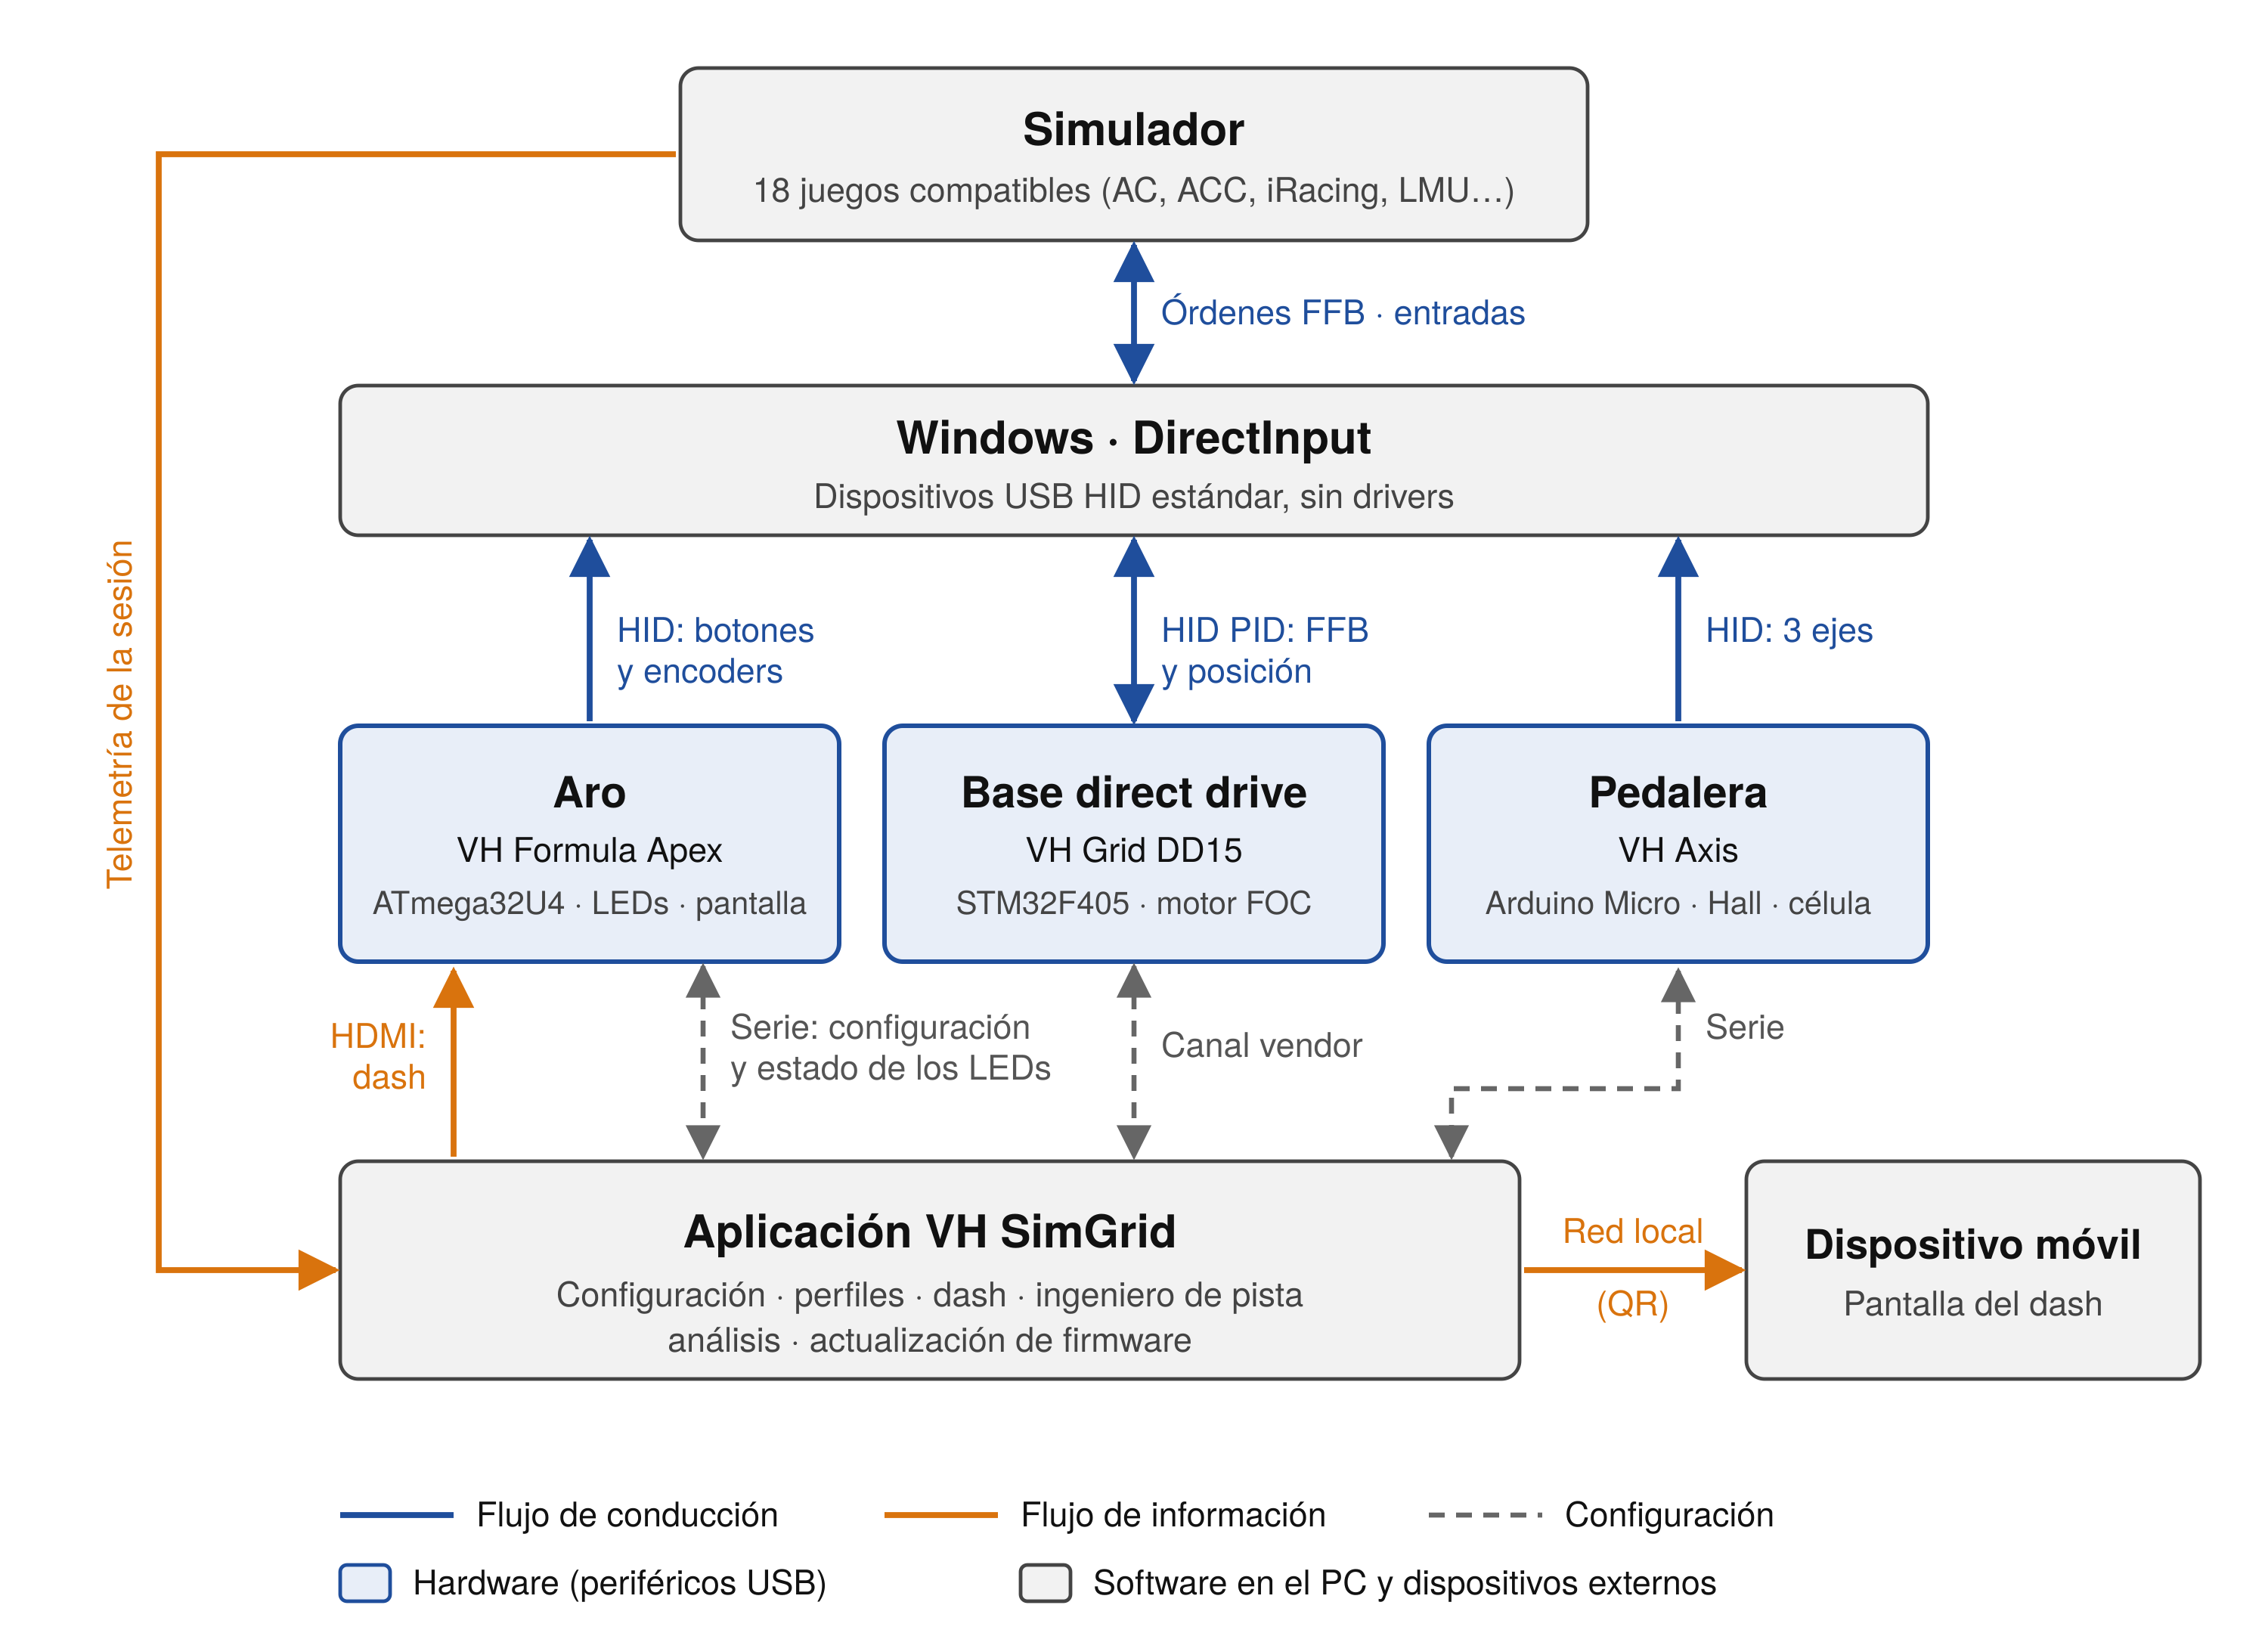
\includegraphics[width=0.84\textwidth,trim=141 39 87 87,clip]{img/diagrama-bloques.png}
	\caption{Diagrama de bloques del ecosistema VH SimGrid. (Fuente propia)}
	\label{fig:diagrama-bloques}
\end{figure}

El diseño separa dos flujos que en la práctica circulan a la vez. El \textbf{flujo de conducción} va del simulador a los periféricos y de los periféricos al simulador, a través de Windows: las órdenes de force feedback, los ejes de los pedales y los botones del aro. El \textbf{flujo de información} va del simulador a la aplicación y de ella al piloto: la telemetría, los LEDs, el dash en la pantalla del aro y en el dispositivo móvil, y la voz del ingeniero. El primero es crítico en tiempo y en seguridad; el segundo enriquece la experiencia. Esta separación es la base del reparto de responsabilidades que se describe a continuación. El detalle de cada canal se recoge en la sección~\ref{sec:protocolos}.

\subsection{Reparto de responsabilidades}
\label{subsec:reparto-responsabilidades}
El principio que guía el diseño es que \textbf{el hardware funciona sin la aplicación abierta}. Cada periférico es autónomo en todo lo necesario para conducir: guarda su propia configuración y se comunica directamente con el simulador a través de los mecanismos estándar de Windows. La aplicación no forma parte del flujo de conducción. Configura los periféricos y añade funciones sobre ellos, pero no es un intermediario por el que deban pasar los datos. Este principio responde directamente a los requisitos RNF19 y RNF20.

Esta decisión responde a tres motivos:

\begin{enumerate}
	\item \textbf{Latencia.} Las órdenes de force feedback viajan del simulador a la base sin pasar por la aplicación. Todo el procesado de la fuerza (curva, ecualizador, efectos base y rango de giro) se ejecuta en el propio firmware, en tiempo real.
	\item \textbf{Robustez y seguridad.} Un cierre inesperado de la aplicación no afecta a la conducción. Las protecciones de la base residen en su firmware y actúan siempre, con independencia del estado del ordenador.
	\item \textbf{Compatibilidad.} Al presentarse como dispositivos HID estándar, los periféricos funcionan en cualquier simulador compatible con DirectInput, incluidos los que la aplicación no admite para telemetría.
\end{enumerate}

En consecuencia, la aplicación se reserva tres tipos de funciones: las de \textbf{configuración} (ajustes en vivo, calibraciones, perfiles y actualización de firmware), las que \textbf{dependen de la telemetría} (los LEDs de revoluciones y eventos del aro, el dash en su pantalla, el ingeniero de pista y la grabación de sesiones) y las de \textbf{gestión} (perfiles automáticos por juego y por coche, y copias de seguridad). La tabla~\ref{tab:reparto-responsabilidades} detalla este reparto.

\begin{table}[H]
	\centering
	\caption{Reparto de responsabilidades entre los periféricos y la aplicación.}
	\label{tab:reparto-responsabilidades}
	\small
	\begin{tabularx}{\textwidth}{@{}>{\raggedright\arraybackslash}p{2.8cm}>{\raggedright\arraybackslash}X>{\raggedright\arraybackslash}X@{}}
		\toprule
		\textbf{Elemento} & \textbf{Funciona sin la aplicación} & \textbf{Requiere la aplicación} \\
		\midrule
		Base VH Grid DD15 &
		Force feedback nativo y efectos (constante, \emph{spring}, \emph{damper}, fricción e inercia); curva, ecualizador y rango de giro; anti-cogging; protecciones de seguridad; ajustes guardados en flash. &
		Modificar los ajustes; cambio automático de perfil; actualización de firmware. \\
		Pedalera VH Axis &
		Lectura de los tres pedales; calibración, curvas y zona muerta guardadas en EEPROM. &
		Calibración guiada; edición de curvas; traza en vivo; actualización de firmware. \\
		Aro VH Formula Apex &
		Botones y encoders como mando estándar; brillo guardado. &
		LEDs de revoluciones y eventos y dash en la pantalla HDMI, que dependen de la telemetría; configuración de luces; actualización de firmware. \\
		Aplicación VH SimGrid &
		--- &
		Telemetría, dash, ingeniero de pista, análisis de sesiones, perfiles y copias de seguridad. \\
		\bottomrule
	\end{tabularx}
\end{table}

Los únicos elementos del hardware que dependen por completo de la aplicación son la tira de LEDs y la pantalla del aro, ya que su contenido procede de la telemetría del simulador. Aun así, el aro sigue siendo plenamente funcional como mando aunque la aplicación no esté abierta.

\section{Diseño de componentes}
\label{sec:diseno-componentes}
Esta sección describe el diseño mecánico y electrónico de los tres periféricos. Para cada uno se recogen los requisitos que debe cumplir, los componentes electrónicos elegidos y el motivo de cada elección, el esquema de conexiones y el concepto mecánico. El proceso de fabricación y montaje de las piezas se detalla en el apartado~\ref{subsec:fabricacion}, y el firmware de cada periférico en la sección~\ref{sec:implementacion-componentes}.

\subsection{Criterios de diseño}
\label{subsec:criterios-diseno}
El diseño de los tres periféricos sigue unos mismos criterios, derivados de los requisitos y de las restricciones generales del capítulo~\ref{cap:requisitos}: un presupuesto propio, una sola persona y un taller doméstico.

\paragraph{Materiales baratos y fáciles de trabajar.}
La industria del automóvil no fabrica sus primeros prototipos con los materiales definitivos. Las formas de un coche nuevo se validan antes en maquetas de arcilla, espuma o madera, que se modelan y corrigen con rapidez y a bajo coste, y solo cuando la forma está decidida se pasa a los materiales y procesos de producción. Este trabajo adopta el mismo enfoque. Cada pieza se valida primero en materiales baratos y fáciles de trabajar, comenzando por poliestireno expandido de alta densidad, después madera y por último PLA impreso en 3D, que permiten comprobar dimensiones, ergonomía y ajustes con muy poca inversión. Solo cuando la pieza está validada se fabrica en su material final, el ABS, más resistente a los esfuerzos y a la temperatura, con un acabado superficial que imita la fibra de carbono. Además, las piezas de acabado liso se tratan con vapor de acetona para conseguir una superficie totalmente pulida.

\paragraph{Componentes comerciales al por menor.}
Toda la electrónica se compone de módulos y componentes que se pueden comprar en tiendas de electrónica o en línea, sin pedidos mínimos ni piezas a medida. Siempre que existe, se elige una plataforma abierta y documentada, como la controladora ODrive o los microcontroladores compatibles con Arduino, de modo que el firmware pueda adaptarse sin depender de un fabricante. Este criterio es el que permite cumplir los requisitos de coste RNF16 y RNF17.

\subsection{Aro VH Formula Apex}
\label{subsec:diseno-aro}
\paragraph{Requisitos.}
El aro debe reunir los mandos que el piloto usa durante la conducción (RF16 y RF17), una tira de LEDs para las revoluciones y los eventos de carrera (RF18 a RF21) y una pantalla en la que se reproduzca el \textit{dash} y desde la que se pueda configurar el equipo (RF22 a RF28). Todo ello debe caber en el espacio reducido de un volante de tipo Fórmula y con un peso contenido, porque toda la masa del aro la tiene que mover el motor de la base y empeora la respuesta del \textit{force feedback}.

La pantalla añade sus propias condiciones (RNF31 a RNF37): una diagonal de entre 4 y 7 pulgadas, integrada sin tapar la visión de la pista ni estorbar a las manos, los botones o las palancas; un peso inferior a 300~g junto con su soporte; una resolución mínima de $800\times480$ píxeles en un panel IPS o equivalente; alimentación por USB, sin fuente adicional; un cableado que soporte el giro completo del volante y el desmontaje rápido del aro; y resistencia a las vibraciones del \textit{force feedback}.

\paragraph{Electrónica.}
El aro se organiza alrededor de un microcontrolador ATmega32U4. Su principal ventaja es el USB integrado, que le permite presentarse a la vez como mando HID, para los botones, y como puerto serie, para la configuración y el estado de los LEDs. Un volante de tipo Fórmula necesita muchos mandos en poco espacio, y el microcontrolador no tiene pines suficientes para leerlos uno a uno. Por eso los pulsadores se leen en matriz, que reduce el número de pines necesarios a la suma de filas y columnas, y los \textit{encoders} se conectan a través de un expansor de entradas y salidas MCP23017 por el bus I2C. La tira de LEDs es de tipo WS2812, en la que cada LED integra su propio controlador y se gobierna individualmente con una única línea de datos.

La pantalla es la excepción: no se conecta al microcontrolador, sino directamente al ordenador por HDMI, como un monitor más que Windows reconoce sin controladores (RF22), y se alimenta por USB (RNF36). Generar el \textit{dash} en el microcontrolador obligaría a usar un procesador mucho más potente y limitaría lo que puede mostrarse. Usando la pantalla como un monitor, el \textit{dash} lo dibuja la aplicación con toda la potencia del ordenador, y el aro solo aporta el panel. La tabla~\ref{tab:componentes-aro} resume los componentes y la figura~\ref{fig:esquema-aro} muestra sus conexiones.

\begin{table}[H]
	\centering
	\caption{Componentes electrónicos del aro VH Formula Apex.}
	\label{tab:componentes-aro}
	\small
	\begin{tabularx}{\textwidth}{@{}>{\raggedright\arraybackslash}p{3.2cm}>{\raggedright\arraybackslash}p{3.6cm}X@{}}
		\toprule
		\textbf{Componente} & \textbf{Función} & \textbf{Motivo de la elección} \\
		\midrule
		Microcontrolador ATmega32U4 & Lee los mandos, gobierna los LEDs y se comunica con el PC & USB nativo, que permite ser mando HID y puerto serie a la vez sin hardware adicional. \\
		Matriz de pulsadores & Botones del aro & Lee muchos pulsadores con pocos pines. \\
		Expansor MCP23017 & Lectura de los \textit{encoders} & Añade entradas por I2C sin ocupar pines del microcontrolador. \\
		Tira de LEDs WS2812 & Barra de RPM y luces por eventos & Cada LED se controla por separado en color y brillo con una sola línea de datos. \\
		Palancas de embrague & Embrague manual desde el aro & Permiten las salidas con punto de mordida (RF17). \\
		Pantalla HDMI & Reproduce el \textit{dash} y el menú de configuración & Se conecta al PC como un monitor y se alimenta por USB; el \textit{dash} lo dibuja la aplicación. \\
		\bottomrule
	\end{tabularx}
\end{table}
\begin{figure}[H]
	\centering
	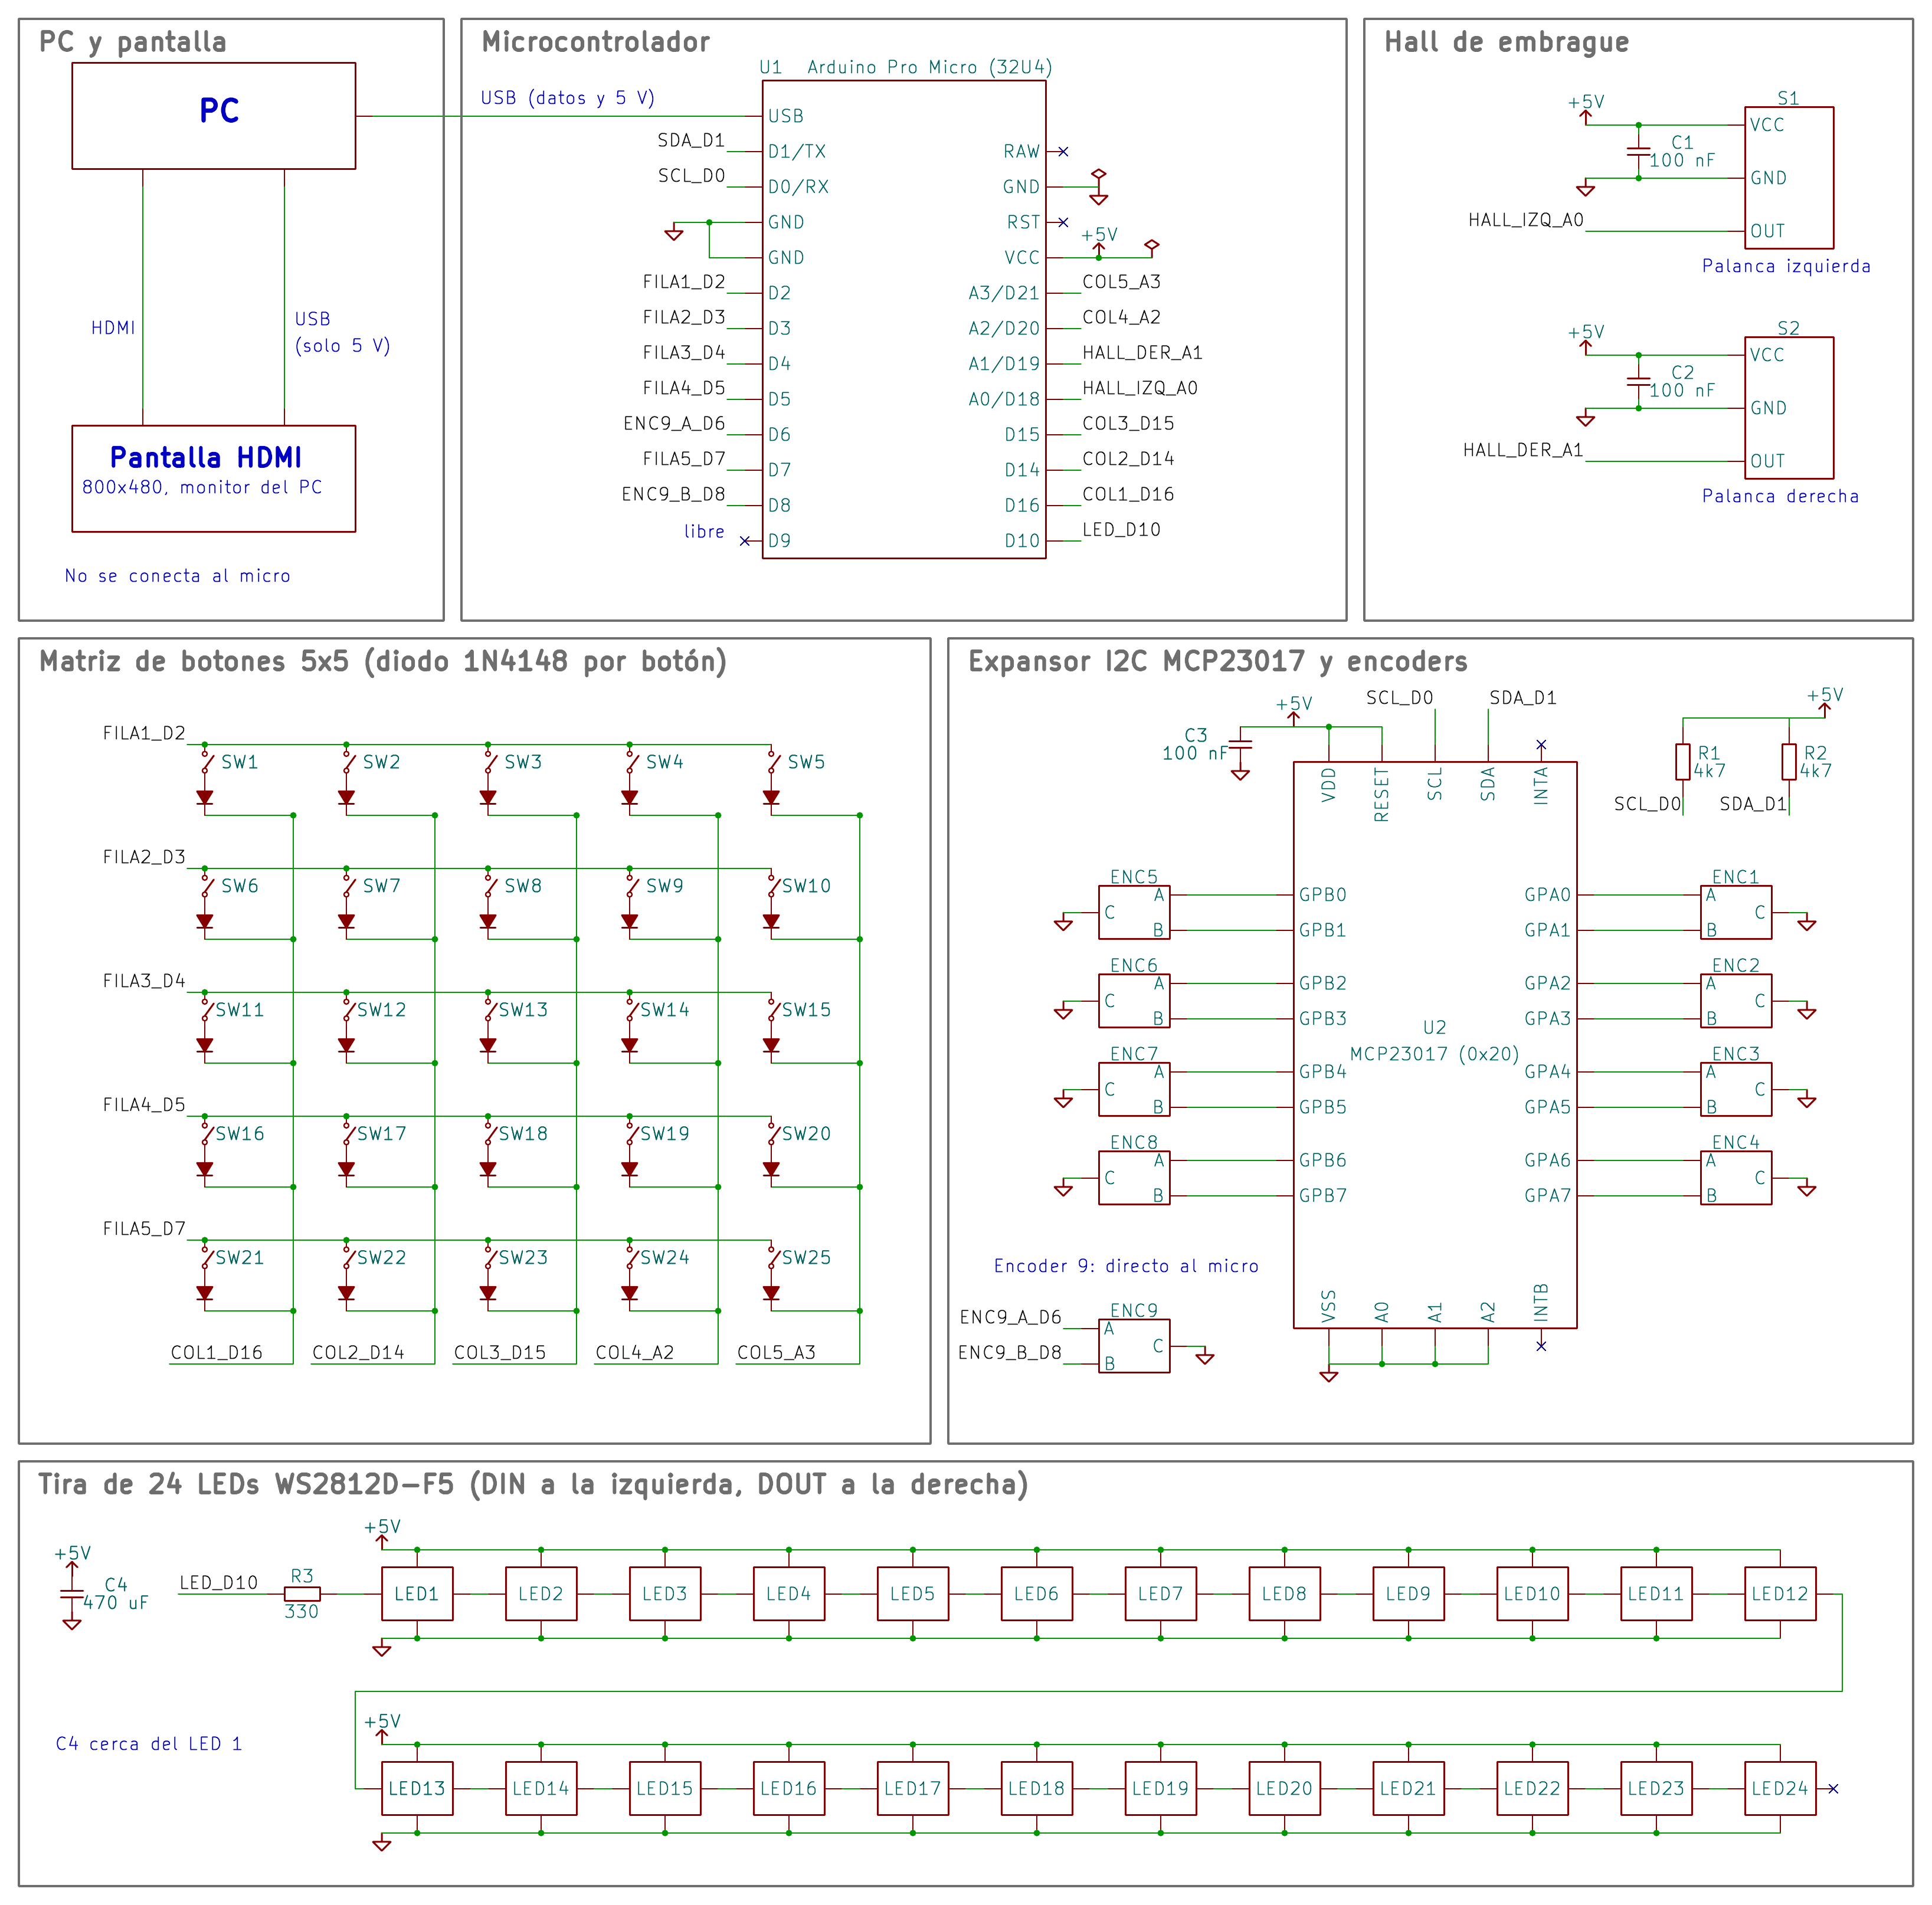
\includegraphics[width=\textwidth]{img/aro-esquema.png}
	\caption{Esquema de conexiones del aro VH Formula Apex. (Fuente propia)}
	\label{fig:esquema-aro}
\end{figure}

\paragraph{Concepto mecánico.}
El aro sigue la forma de los volantes de los monoplazas actuales, los cuales se caracterizan por su pequeño diámetro, con dos empuñaduras laterales y los mandos concentrados en el frontal, alrededor de la pantalla, para que el piloto los alcance con los pulgares sin soltar las manos. La pantalla ocupa el centro del frontal, a la altura de la vista pero por debajo de la línea de visión hacia la pista (RNF31), y su soporte forma parte del propio cuerpo del aro para resistir las vibraciones (RNF37). La tira de LEDs se sitúa en la parte superior, en la línea de visión del piloto hacia la pista. Las levas de cambio y las palancas de embrague van en la parte trasera, al alcance de los dedos. El cuerpo se divide en piezas que alojan la electrónica en su interior, y el aro se une a la base mediante un sistema de desmontaje rápido por el que pasan también los cables de USB y HDMI (RNF35). La figura~\ref{fig:render-aro} muestra el diseño.

\begin{figure}[H]
	\centering
	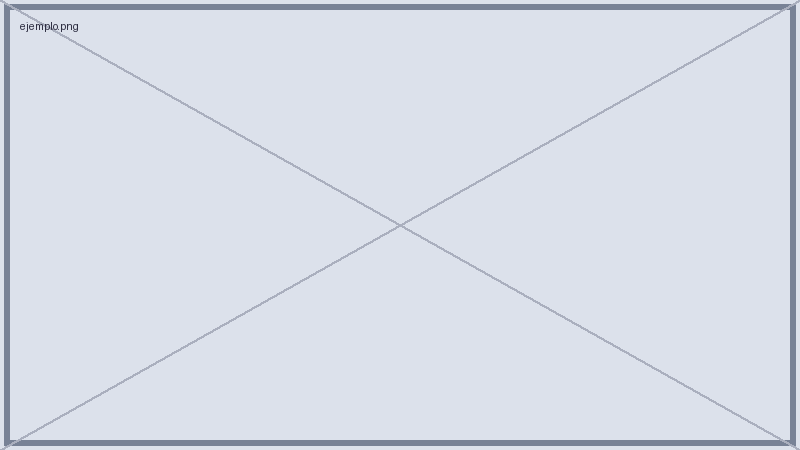
\includegraphics[width=0.8\textwidth]{img/ejemplo.png}
	\caption{Diseño del aro VH Formula Apex. (Fuente propia)}
	\label{fig:render-aro}
\end{figure}

\subsection{Pedalera VH Axis}
\label{subsec:diseno-pedalera}
\paragraph{Requisitos.}
La pedalera debe presentarse como un mando de tres ejes, con el acelerador y el embrague medidos por posición y el freno por fuerza (RF11), y guardar su configuración en su propia memoria (RF14 y RNF19). Debe leer los pedales a unos 1000~Hz sin un retardo perceptible (RNF3). Mecánicamente, el freno debe soportar de forma repetida la fuerza máxima de la célula de carga sin deformarse ni perder la calibración (RNF23).

\paragraph{Electrónica.}
La pedalera usa un Arduino Micro, que monta el mismo ATmega32U4 que el aro y comparte con él la ventaja del USB nativo, es mando HID de tres ejes y puerto serie de configuración a la vez. El acelerador y el embrague miden su recorrido con sensores de efecto Hall, que detectan la posición de un imán sin contacto y no se desgastan. Su salida es analógica y se lee directamente con el conversor del microcontrolador.

El freno mide la fuerza con una célula de carga de 200~kg. Su señal es del orden de milivoltios y necesita amplificarse antes de digitalizarla. La solución habitual en proyectos de este tipo es el módulo HX711, un conversor de alta resolución pensado para básculas, pero su frecuencia de muestreo máxima, de 80 muestras por segundo, es muy inferior a los 1000~Hz que exige el requisito RNF3. Por eso, y tras las pruebas realizadas, se ha decidido usar en su lugar un amplificador de instrumentación INA333, que amplifica la señal del puente de la célula de forma continua y la entrega al conversor del microcontrolador, que puede leerla a la misma frecuencia que los otros dos pedales. La resolución que se pierde frente al HX711 se compensa con el filtrado digital de la señal. La tabla~\ref{tab:componentes-pedalera} resume los componentes y la figura~\ref{fig:esquema-pedalera} muestra sus conexiones.

\begin{table}[H]
	\centering
	\caption{Componentes electrónicos de la pedalera VH Axis.}
	\label{tab:componentes-pedalera}
	\small
	\begin{tabularx}{\textwidth}{@{}>{\raggedright\arraybackslash}p{3.2cm}>{\raggedright\arraybackslash}p{3.6cm}X@{}}
		\toprule
		\textbf{Componente} & \textbf{Función} & \textbf{Motivo de la elección} \\
		\midrule
		Arduino Micro (ATmega32U4) & Lee los sensores y se comunica con el PC & USB nativo, que permite ser mando HID y puerto serie a la vez. \\
		Sensores de efecto Hall & Recorrido del acelerador y del embrague & Miden sin contacto, sin desgaste ni ruido mecánico. \\
		Célula de carga de 200~kg & Fuerza sobre el freno & Mide la magnitud que controla el piloto en una frenada real. \\
		Amplificador INA333 & Amplifica la señal de la célula & Permite leer el freno a unos 1000~Hz, frente a las 80 muestras por segundo del HX711. \\
		\bottomrule
	\end{tabularx}
\end{table}
\begin{figure}[H]
	\centering
	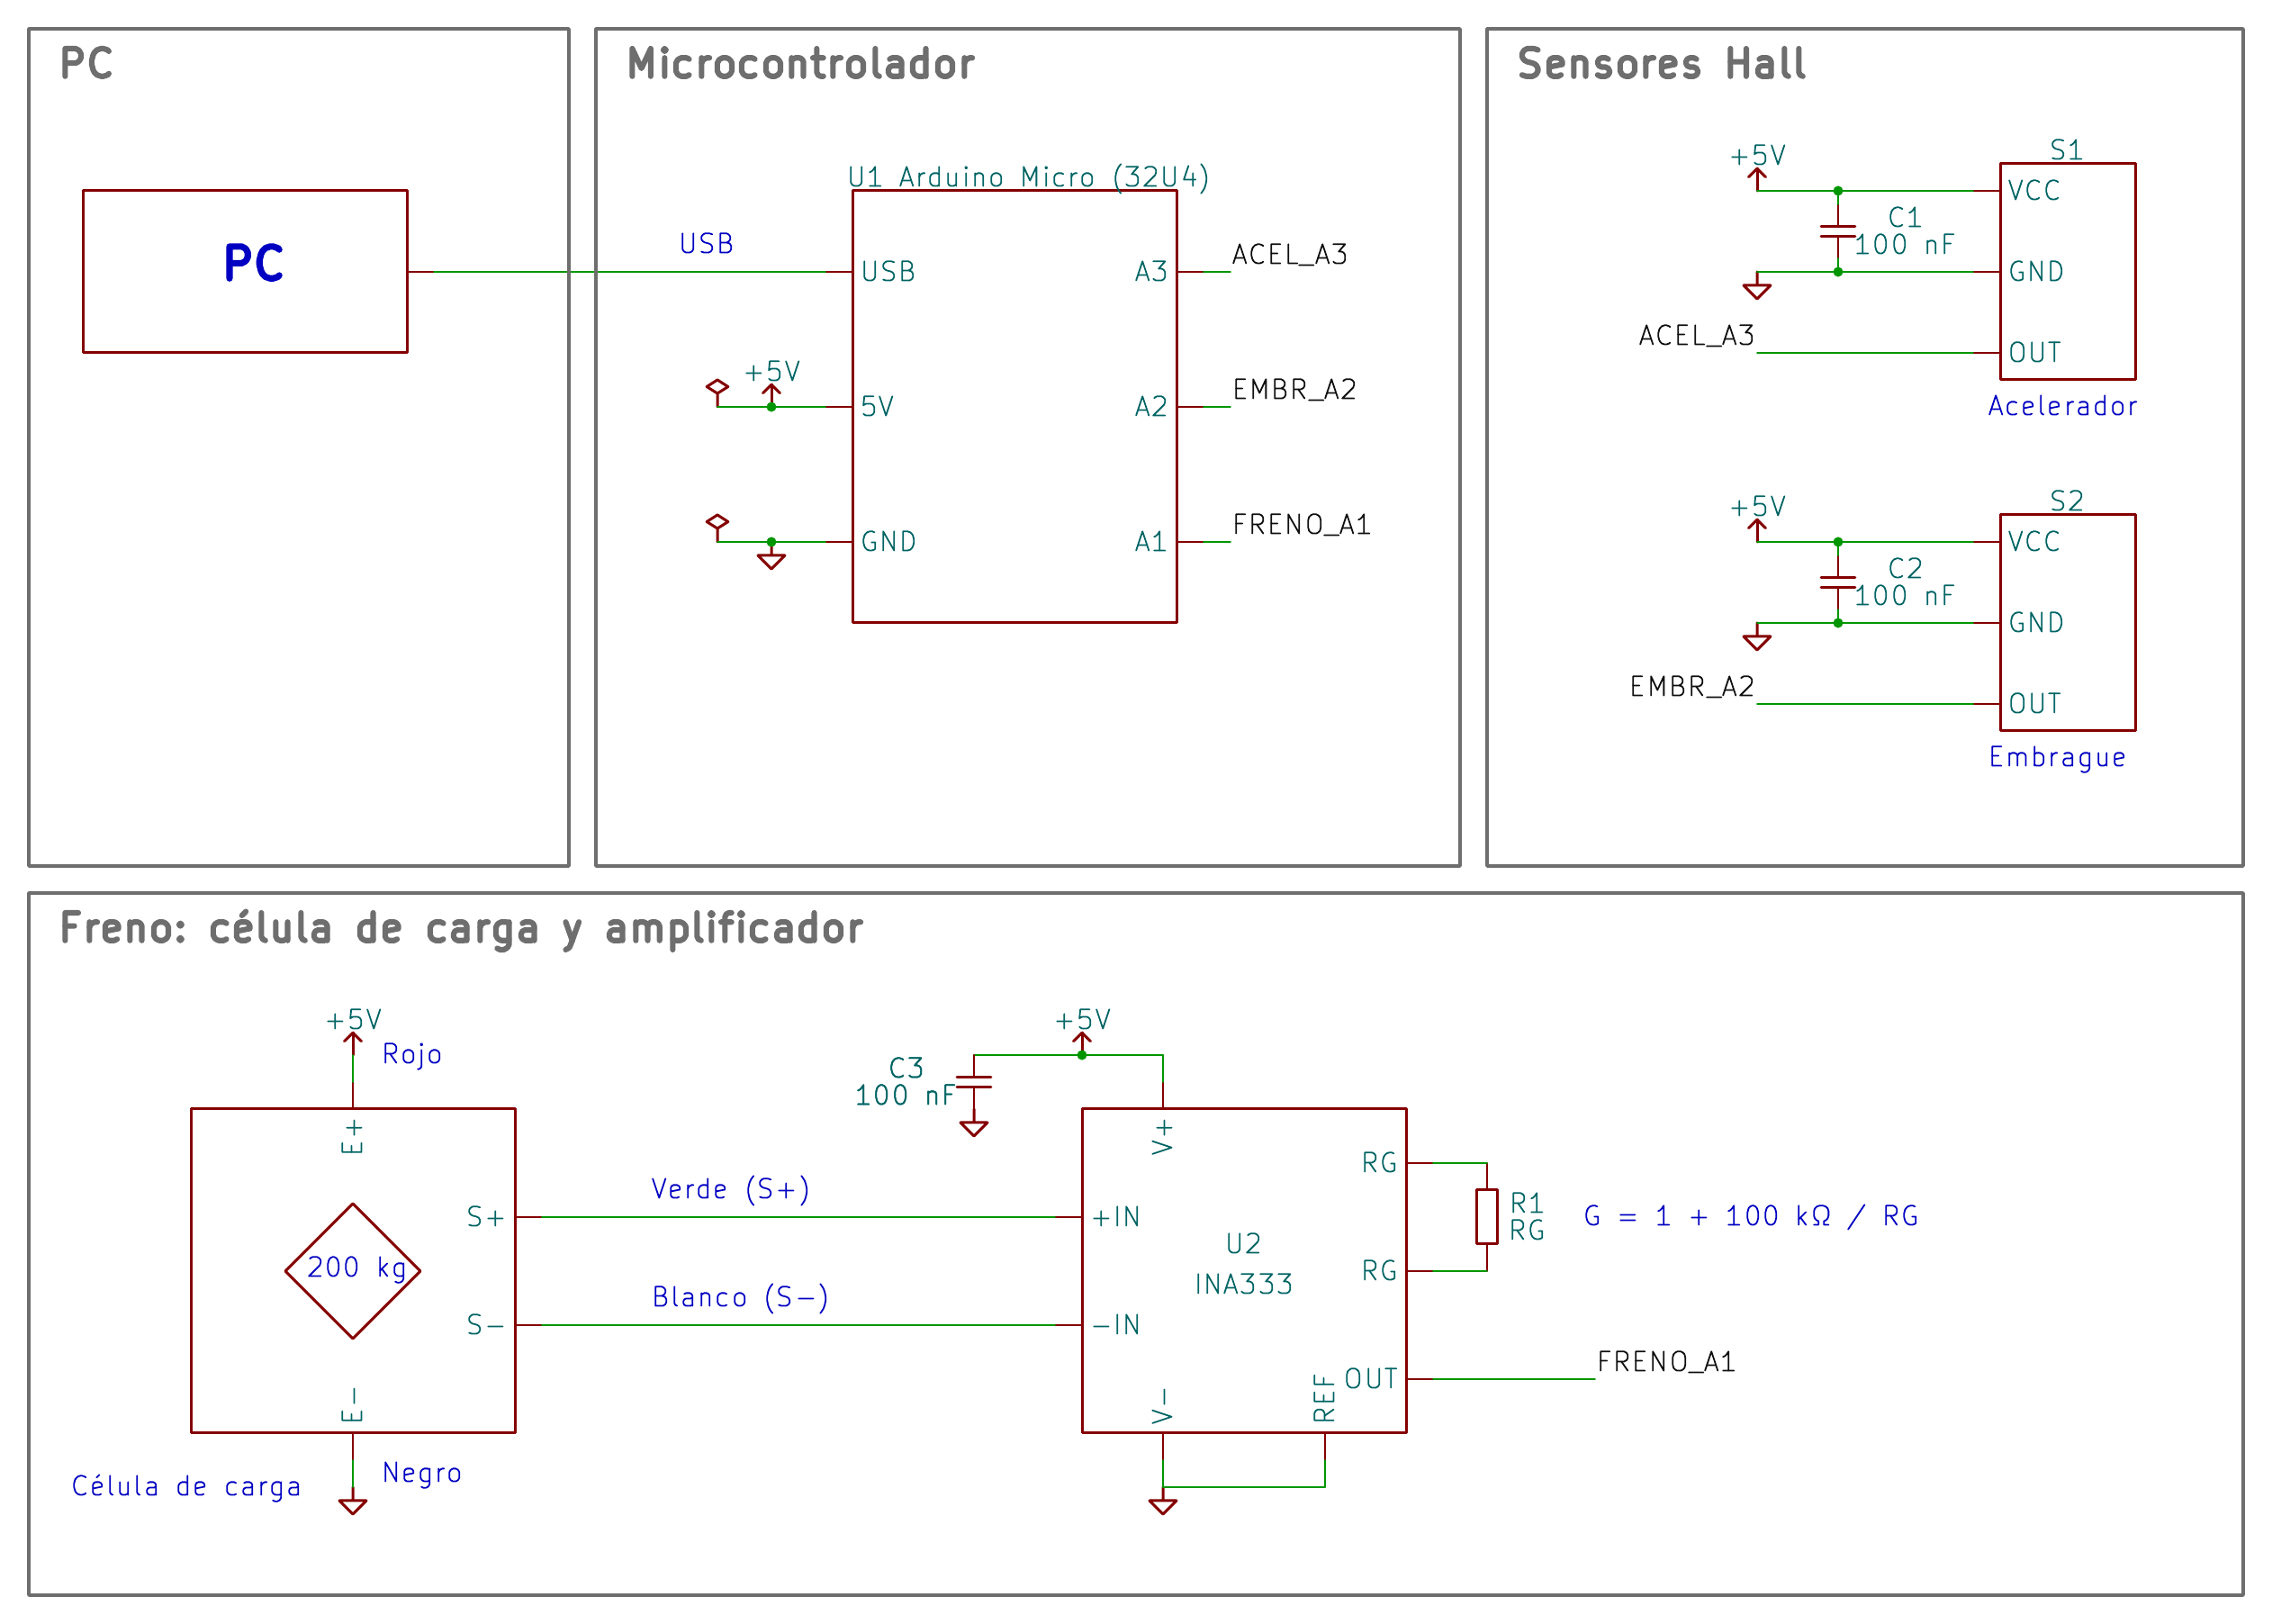
\includegraphics[width=\textwidth]{img/pedalera-esquema.png}
	\caption{Esquema de conexiones de la pedalera VH Axis. (Fuente propia)}
	\label{fig:esquema-pedalera}
\end{figure}

\paragraph{Concepto mecánico.}
Cada pedal es un brazo que gira sobre un eje fijado a la base de la pedalera, con su sensor en el propio pivote o en el recorrido del brazo. El acelerador y el embrague recuperan su posición con un muelle, porque lo que importa en ellos es el recorrido. En el freno, en cambio, el pedal apenas debe moverse: el brazo empuja contra la célula de carga a través de un elemento elástico que le da una resistencia progresiva, de modo que el pie sienta una dureza creciente parecida a la de un freno hidráulico. El brazo del freno y su apoyo sobre la célula se dimensionan para la fuerza máxima de esta, de modo que una frenada a fondo no deforme la estructura ni desplace la célula (RNF23). Los tres pedales se montan sobre una base común, con la separación y la inclinación de un pedalier de competición. La figura~\ref{fig:render-pedalera} muestra el diseño.

\begin{figure}[H]
	\centering
	% TODO: render CAD de la pedalera
	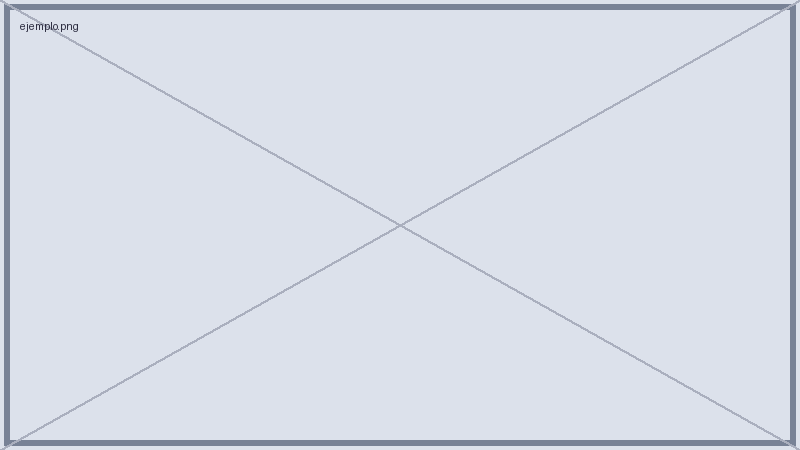
\includegraphics[width=0.8\textwidth]{img/ejemplo.png}
	\caption{Diseño de la pedalera VH Axis. (Fuente propia)}
	\label{fig:render-pedalera}
\end{figure}
% TODO: elemento elástico del freno (elastómero, muelles...) y material de la estructura y los brazos.

\subsection{Base VH Grid DD15}
\label{subsec:diseno-base}

\paragraph{Requisitos.}
La base debe ser reconocida como un volante con \textit{force feedback} nativo (RF1), reproducir los efectos de DirectInput (RF2) y ofrecer un rango de giro de hasta 1440° (RF3). Debe atender los informes de fuerza cada milisegundo y aplicar el par en menos de 2~ms desde que llegan (RNF1 y RNF2). Por encima de todo, debe ser segura: un motor capaz de mover el volante con fuerza puede lesionar al piloto si el control falla, por lo que la electrónica debe permitir vigilar en todo momento la velocidad, la corriente y la temperatura del motor y de la controladora, y cortar el par ante cualquier anomalía (RNF8 a RNF14).

\paragraph{Electrónica.}
La base usa una transmisión \textit{direct drive}, en la que el aro va unido directamente al motor, sin engranajes ni correas que filtren o retrasen la fuerza. Esto exige un motor que dé mucho par a baja velocidad. El motor de buje de un patinete eléctrico cumple ese requisito: es un motor sin escobillas pensado para mover la rueda directamente, con muchos polos y un par elevado a pocas revoluciones, y su precio es una fracción del de los motores de las bases comerciales. Su inconveniente es un rizado magnético (\textit{cogging}) apreciable, que se nota en las manos como pequeños escalones al girar. En lugar de buscar un motor más caro, se decide corregirlo por software con una calibración anti-cogging (RF8), que se describe en el apartado~\ref{subsec:fw-base}.

Para controlar el motor se usa una controladora MKS ODrive Mini, compatible con el proyecto de código abierto ODrive. Integra un microcontrolador STM32F405, con USB nativo y potencia de cálculo suficiente para ejecutar el control vectorial (FOC) del motor y, a la vez, el dispositivo HID PID y el motor de efectos, de modo que toda la base funciona con una sola placa. La posición del volante se mide con un encoder óptico de alta resolución, necesario para el control FOC y para que la fuerza se calcule con precisión incluso en movimientos muy pequeños. El motor no lleva sonda de temperatura: el firmware estima su calentamiento a partir de la corriente aplicada (modelo I$^2$t) y reduce el par de forma progresiva antes de que se sobrecaliente. La temperatura de los transistores de la controladora sí se mide, con el termistor NTC que integra la placa (RNF9). La fuente de alimentación se dimensiona para la corriente de pico de la controladora, y la energía que el motor devuelve al frenar se limita para no dañarla (RNF11). La tabla~\ref{tab:componentes-base} resume los componentes y la figura~\ref{fig:esquema-base} muestra sus conexiones.

\begin{table}[H]
	\centering
	\caption{Componentes electrónicos de la base VH Grid DD15.}
	\label{tab:componentes-base}
	\small
	\begin{tabularx}{\textwidth}{@{}>{\raggedright\arraybackslash}p{3.2cm}>{\raggedright\arraybackslash}p{3.6cm}X@{}}
		\toprule
		\textbf{Componente} & \textbf{Función} & \textbf{Motivo de la elección} \\
		\midrule
		Motor de buje de patinete eléctrico & Genera el par sobre el volante & Mucho par a baja velocidad y muy bajo coste; su \textit{cogging} se corrige por software. \\
		Controladora MKS ODrive Mini (STM32F405) & Control FOC del motor, HID PID y efectos & Plataforma abierta, USB nativo y potencia para todo el firmware en una sola placa. \\
		Encoder óptico & Posición del volante & Alta resolución, necesaria para el control FOC y la precisión de la fuerza. \\
		Termistor NTC (integrado en la controladora) & Temperatura de los transistores & Permite limitar la corriente si la placa se calienta (RNF9). \\
		Fuente de alimentación & Alimenta la controladora y el motor & Dimensionada para la corriente de pico de la controladora. \\
		\bottomrule
	\end{tabularx}
\end{table}

\begin{figure}[H]
	\centering
	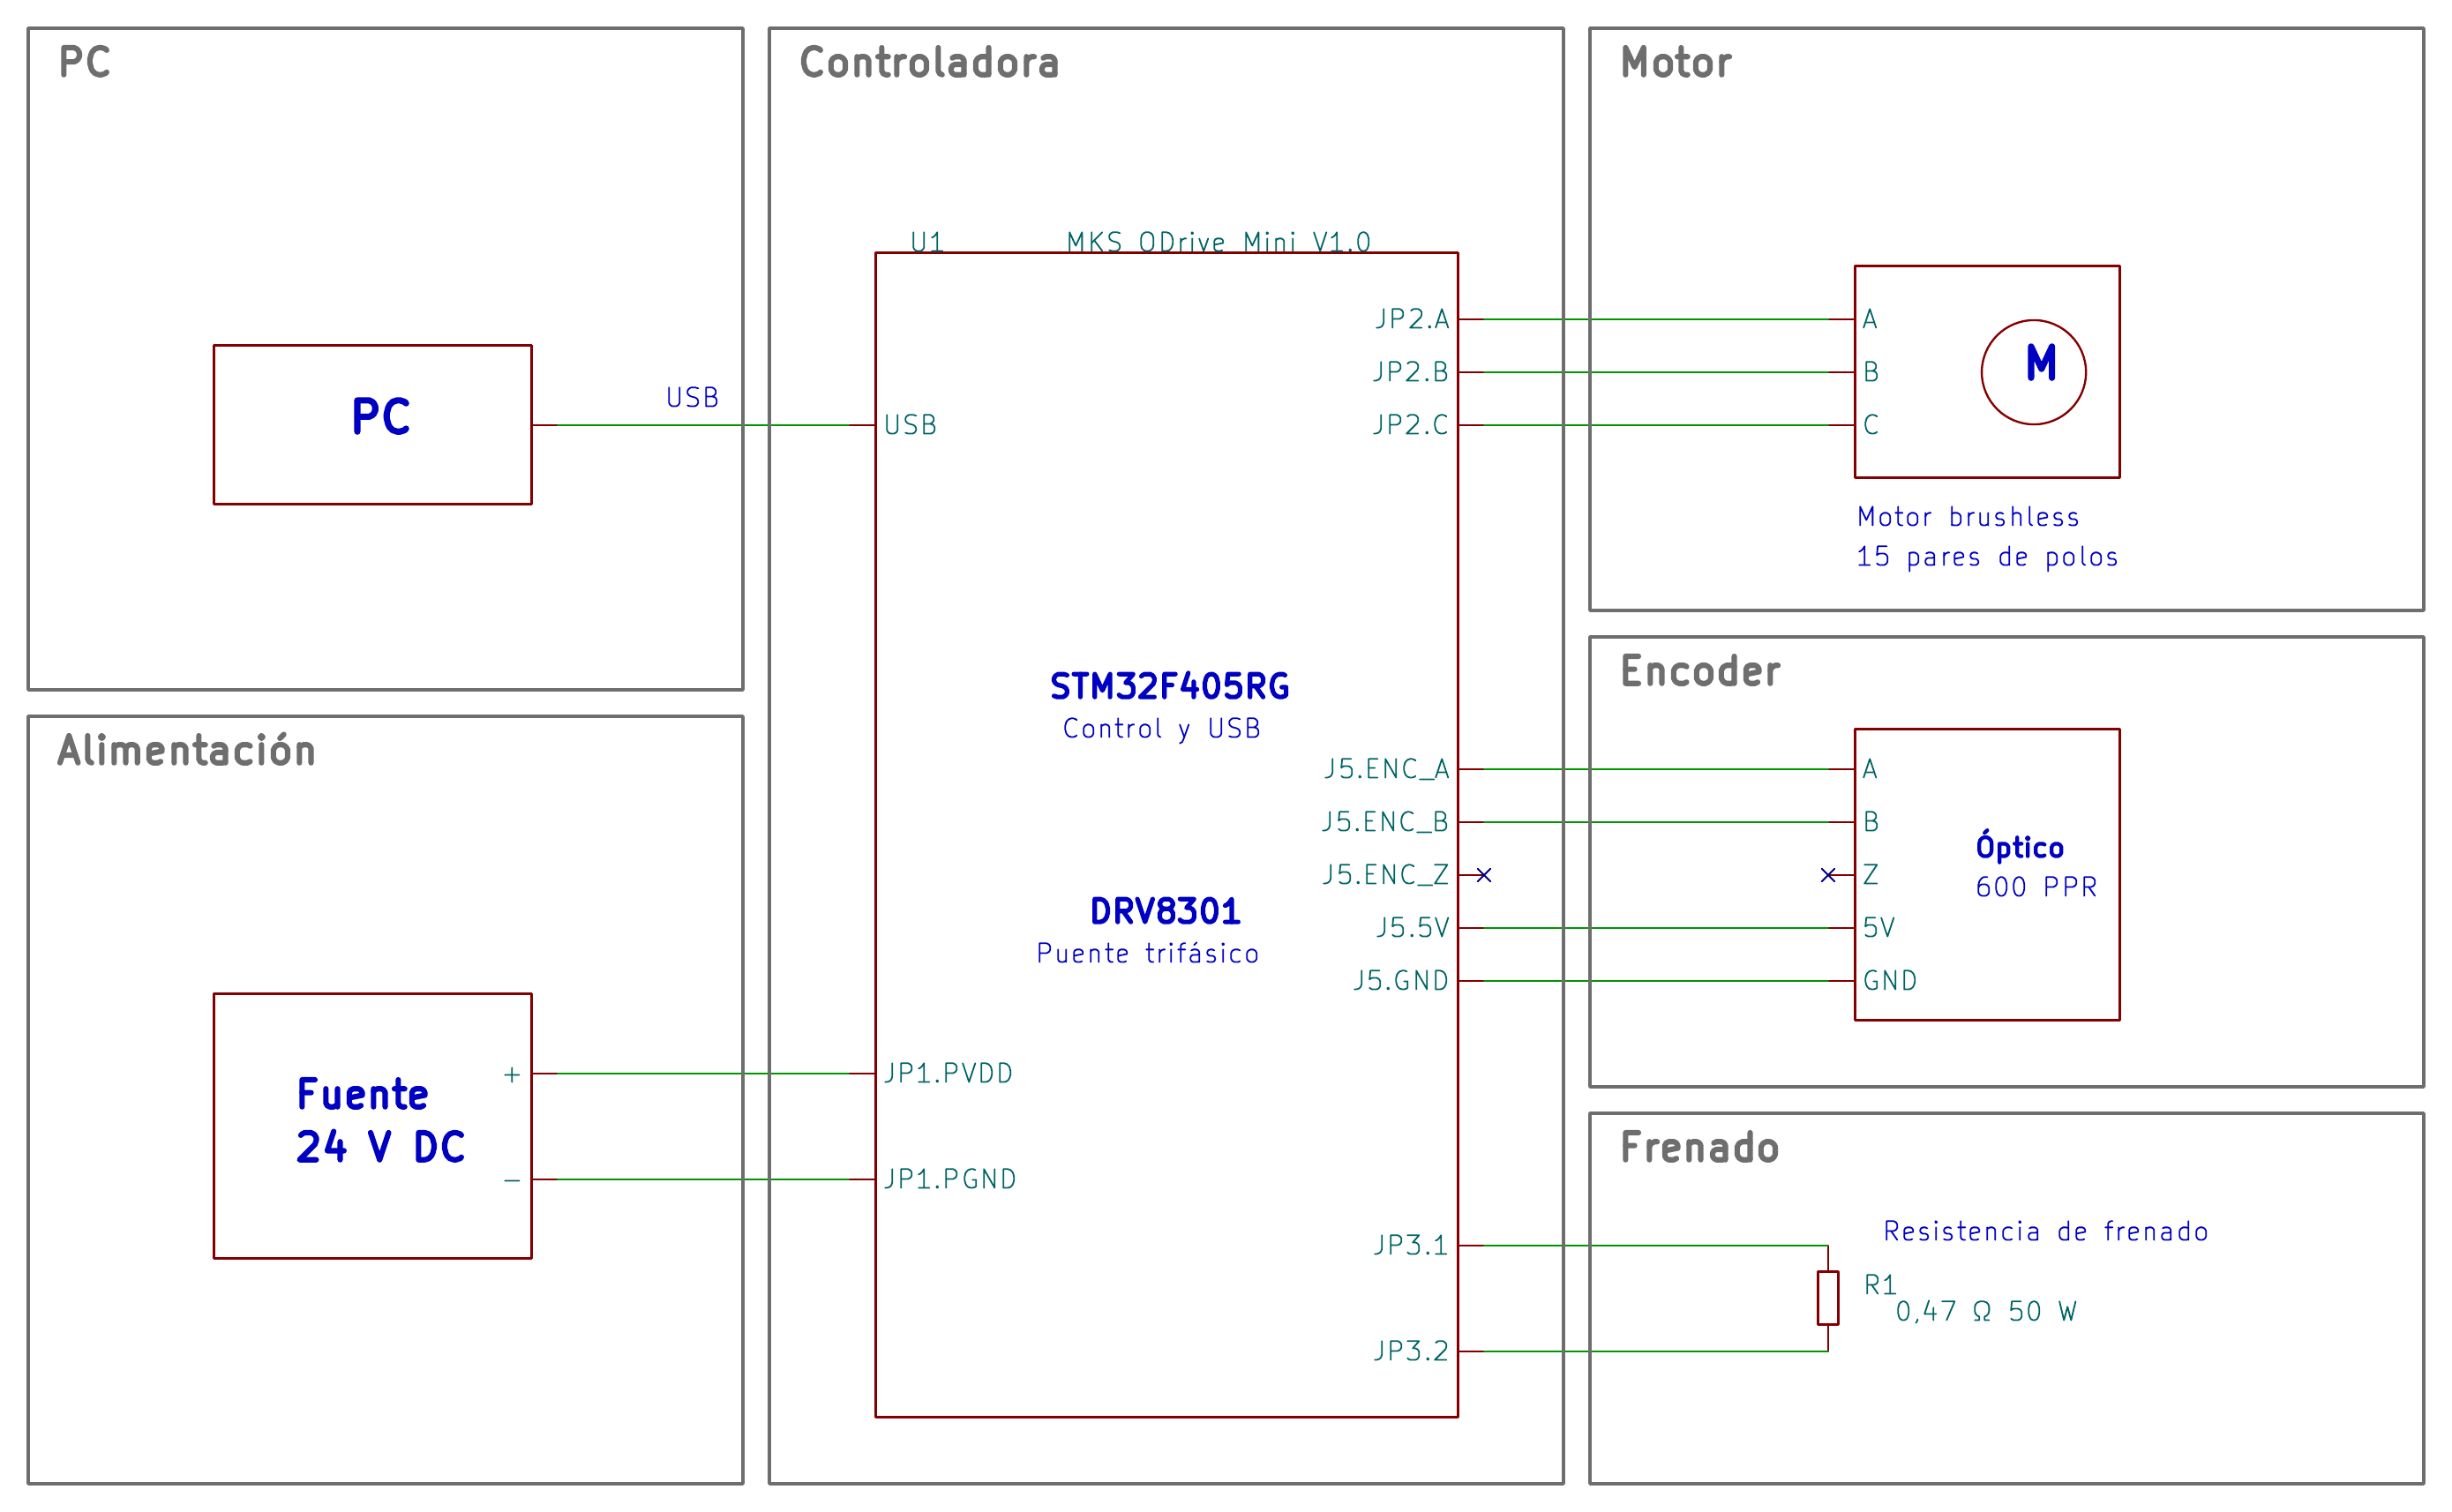
\includegraphics[width=\textwidth]{img/base-esquema.png}
	\caption{Esquema de conexiones de la base VH Grid DD15. (Fuente propia)}
	\label{fig:esquema-base}
\end{figure}

\paragraph{Concepto mecánico.}
En un motor de buje el eje es fijo y lo que gira es la carcasa exterior, que en el patinete es la propia rueda. El diseño aprovecha esta disposición: el eje del motor se fija a la estructura de la base y el aro se une a la carcasa giratoria mediante un adaptador con el sistema de desmontaje rápido, de modo que el par del motor llega al volante sin ningún elemento intermedio. La estructura aloja el motor, la controladora y el encoder, y se ancla con firmeza al puesto de conducción. La figura~\ref{fig:render-base} muestra el diseño.

\begin{figure}[H]
	\centering
	% TODO: render CAD de la base
	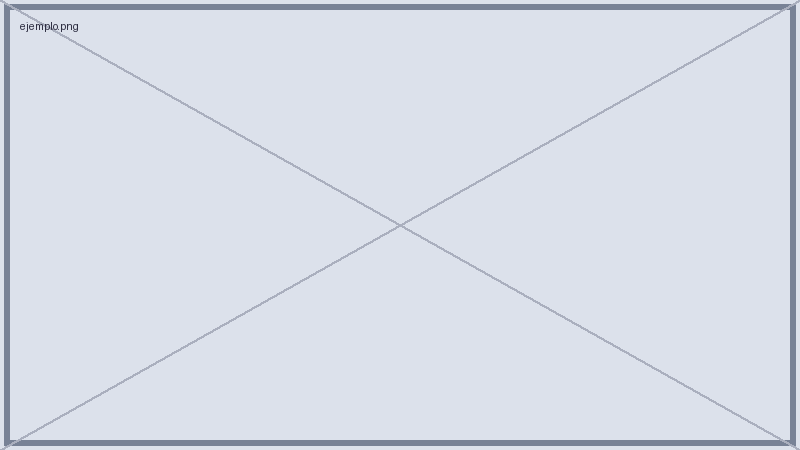
\includegraphics[width=0.8\textwidth]{img/ejemplo.png}
	\caption{Diseño de la base VH Grid DD15. (Fuente propia)}
	\label{fig:render-base}
\end{figure}

\section{Arquitectura tecnológica}
\label{sec:arquitectura-tecnologica}
El sistema tiene dos tipos de software: por un lado, el firmware que se ejecuta en cada periférico y, por otro, la aplicación de escritorio. Ambos se organizan en capas, de modo que cada capa solo depende de la que tiene debajo y ofrece sus servicios a la capa que tiene por encima. Esta separación permite cambiar una parte sin tocar el resto, por ejemplo sustituir un sensor afecta solo a la capa más baja del firmware, y añadir un simulador nuevo afecta solo al módulo de telemetría de la aplicación, como exige el requisito RNF43. Esta sección describe la organización de ambos.

\subsection{Firmware}
\label{subsec:arq-firmware}
Los tres periféricos comparten una misma estructura en capas, aunque cada uno la llena con funciones distintas según su papel. La figura~\ref{fig:capas-firmware} resume esta estructura y la tabla~\ref{tab:capas-firmware} describe la función de cada capa.

\begin{figure}[H]
	\centering
	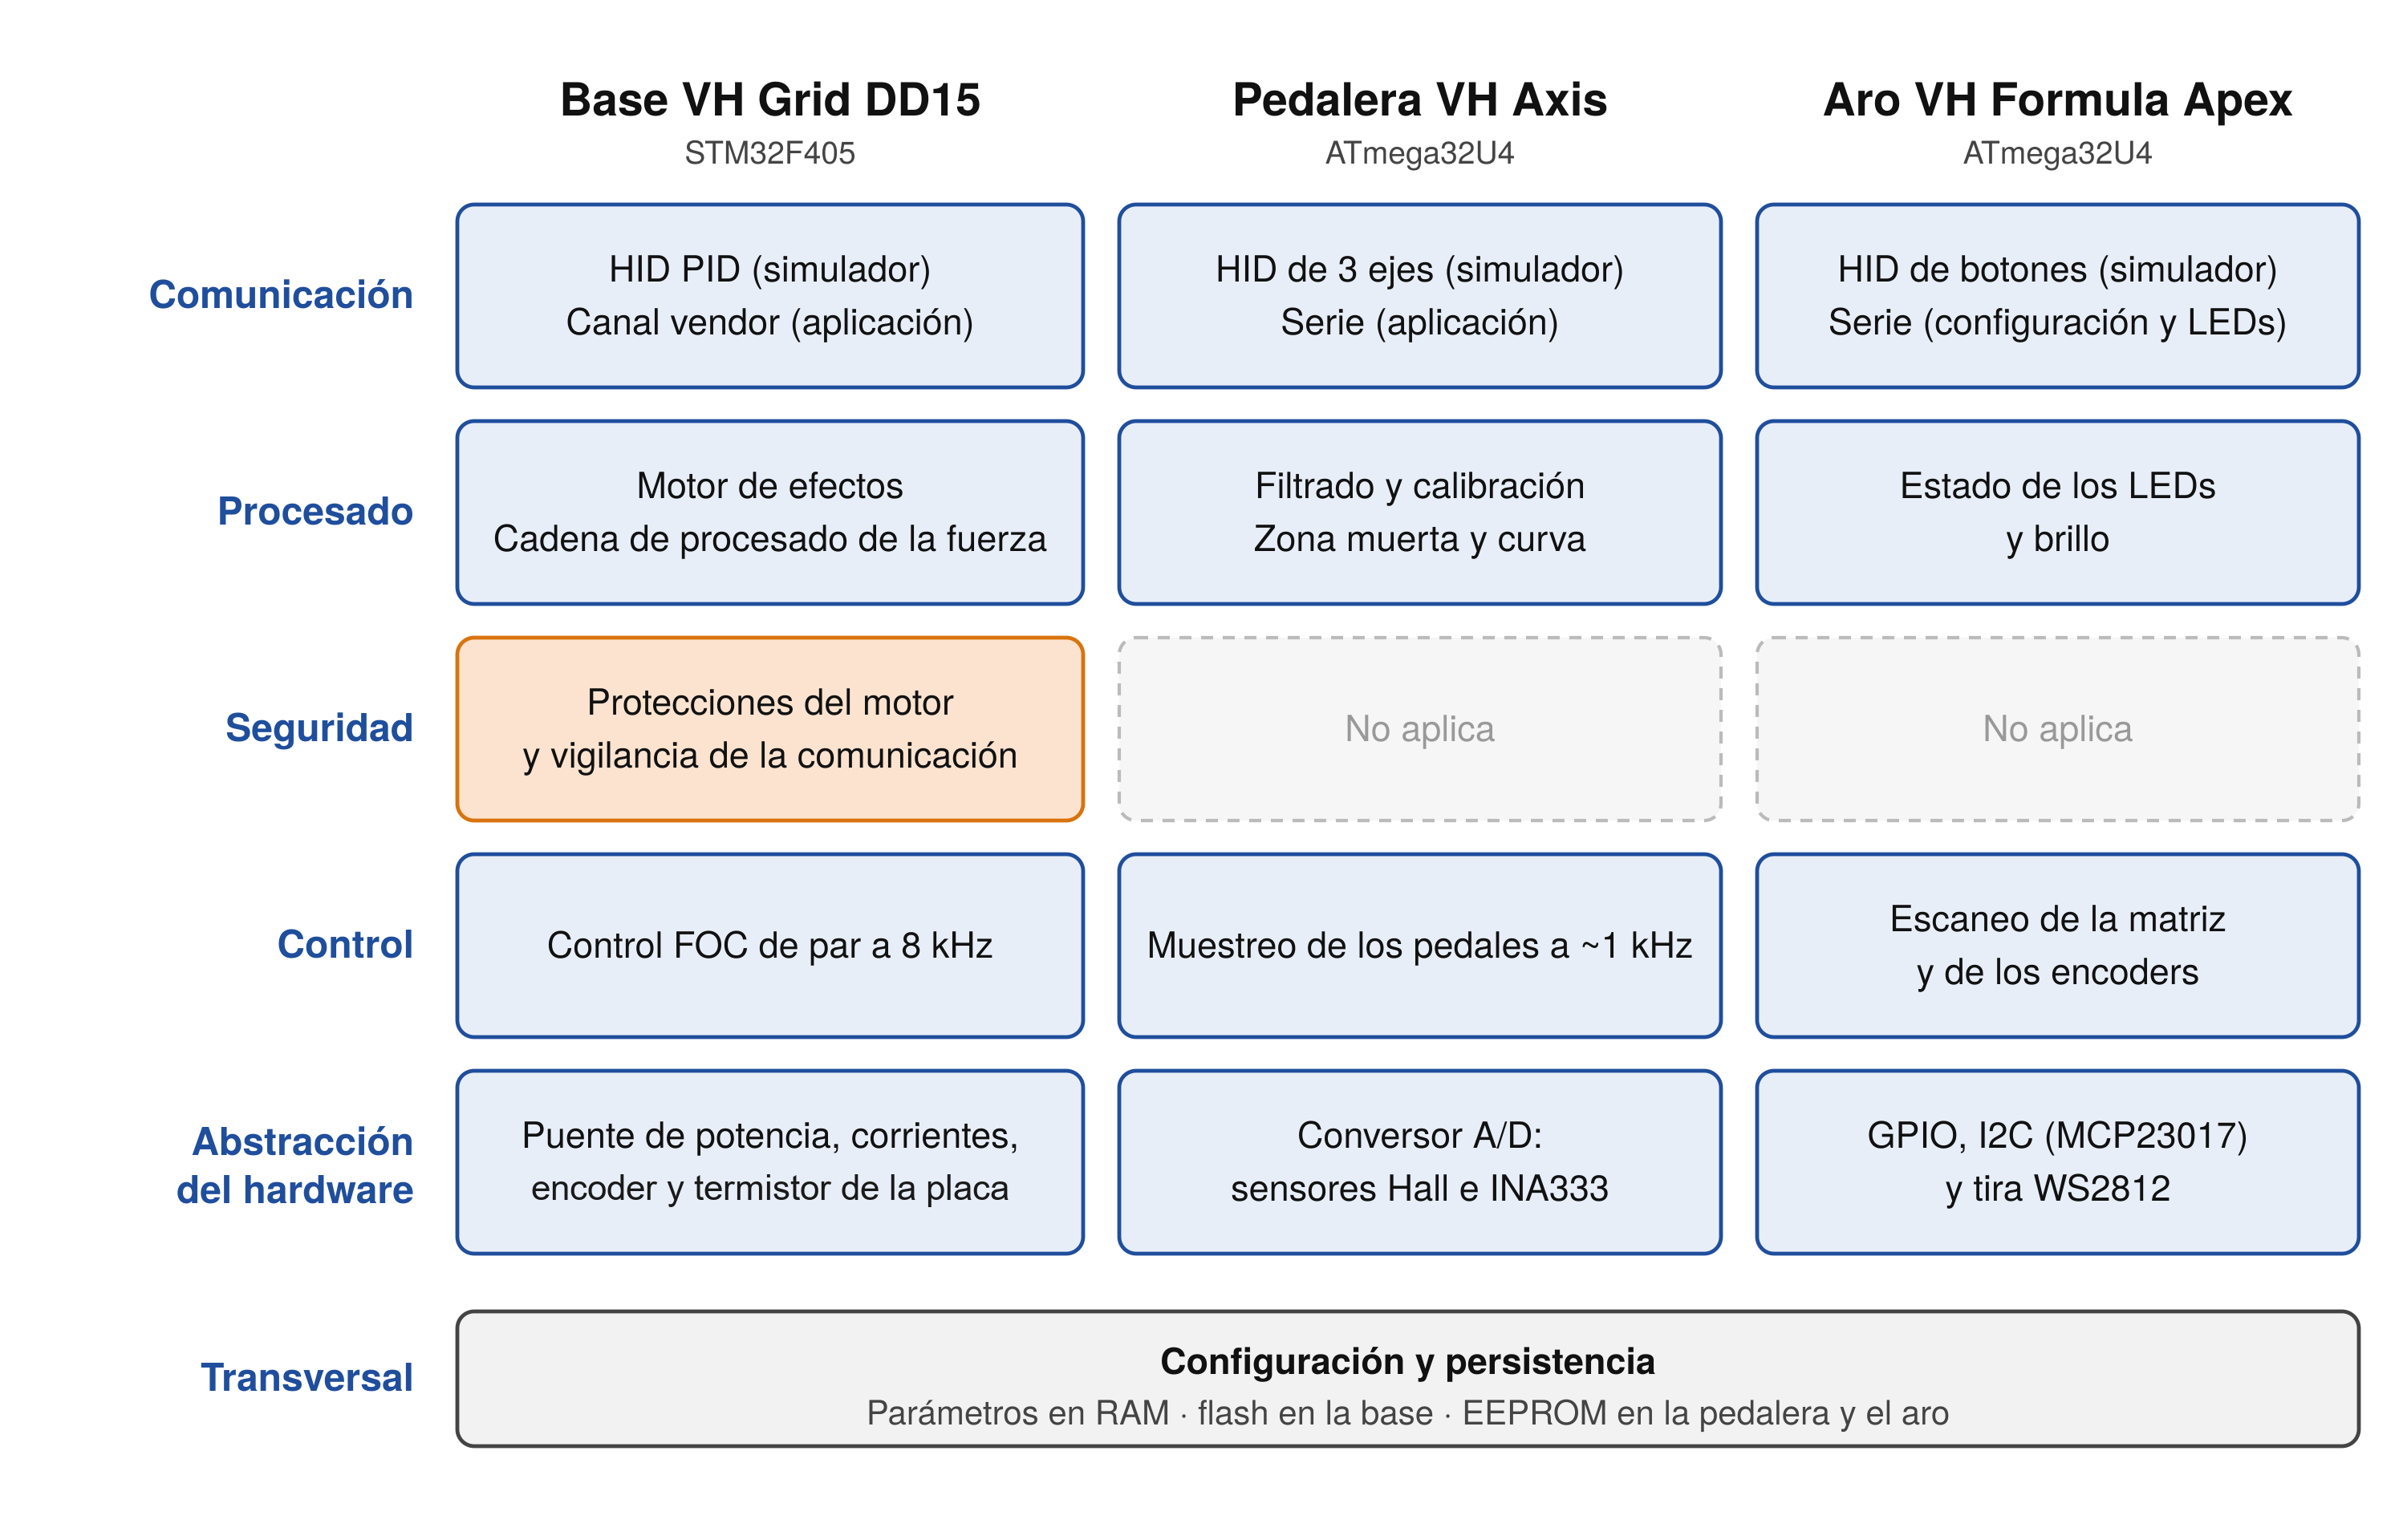
\includegraphics[width=\textwidth]{img/capas-firmware.png}
	\caption{Arquitectura en capas del firmware de los tres periféricos. (Fuente propia)}
	\label{fig:capas-firmware}
\end{figure}

\begin{table}[H]
	\centering
	\caption{Capas del firmware y su función.}
	\label{tab:capas-firmware}
	\small
	\begin{tabularx}{\textwidth}{@{}>{\raggedright\arraybackslash}p{3.2cm}X@{}}
		\toprule
		\textbf{Capa} & \textbf{Función} \\
		\midrule
		Comunicación & Presenta el periférico ante el ordenador con dos canales simultáneos: el HID, que usa el simulador, y el de configuración, que usa la aplicación. En la pedalera y el aro son dos interfaces de un dispositivo USB compuesto; en la base, informes distintos dentro de una sola interfaz HID. \\
		Procesado & Transforma las lecturas o las órdenes recibidas según los ajustes del usuario: el motor de efectos y la cadena de procesado de la fuerza en la base, el filtrado, la calibración y las curvas en la pedalera, y el estado y el brillo de los LEDs en el aro. \\
		Seguridad & Solo en la base. Vigila el estado del motor y de la comunicación, y limita o anula el par ante cualquier anomalía. \\
		Control & Ejecuta el lazo de tiempo real de cada periférico a una frecuencia fija: el control FOC del motor, el muestreo de los pedales o el escaneo de los mandos. \\
		Abstracción del hardware & Encapsula los periféricos del microcontrolador (conversor A/D, temporizadores, PWM, GPIO, I2C y USB) y los sensores y actuadores conectados a ellos. \\
		Configuración y persistencia & Capa transversal. Mantiene los parámetros activos en RAM, los expone a la capa de comunicación para su lectura y modificación en vivo y los guarda en memoria no volátil. \\
		\bottomrule
	\end{tabularx}
\end{table}

\paragraph{Separación entre el juego y la configuración.}
Cada periférico ofrece un canal HID estándar para el simulador y otro independiente para la aplicación. En la pedalera y el aro son dos interfaces de un dispositivo USB compuesto, HID y puerto serie. En la base, que tiene una sola interfaz HID, el canal de configuración es un informe \textit{vendor} propio, separado de los informes PID. Gracias a esta separación, la aplicación puede leer y cambiar ajustes mientras el juego está en marcha sin interferir con los informes de entrada ni con las órdenes de fuerza (RF30), y el periférico funciona como un mando normal aunque la interfaz de configuración no se use nunca (RNF20).

\paragraph{Parámetros en RAM y escritura bajo demanda.}
La capa transversal de configuración mantiene una única copia de los parámetros activos en RAM, que es la que leen las capas de procesado y control. Un cambio llegado desde la aplicación se aplica sobre esa copia y tiene efecto inmediato (RNF5). La escritura en memoria no volátil se hace aparte y solo cuando un valor ha cambiado, para no agotar los ciclos de escritura de la flash y la EEPROM (RNF22). Al arrancar, el periférico carga esa copia guardada, de modo que conserva su configuración aunque se conecte a otro ordenador (RNF19). El contenido exacto de lo que se guarda se describe en la sección~\ref{sec:persistencia}.

\paragraph{Base VH Grid DD15.}
La base es el periférico con la escritura más exigente porque debe atender a la vez tres tipos de trabajo con plazos muy distintos. El \textbf{lazo de control} se ejecuta a 8~kHz con la máxima prioridad: lee la corriente y la posición del motor y calcula la tensión de cada fase mediante el control FOC. Ninguna otra tarea puede retrasarlo, porque un retraso lo notaría el piloto y podría comprometer su seguridad. La \textbf{tarea de fuerza} se ejecuta cada milisegundo (RNF1): recoge los informes recibidos por USB, calcula la fuerza, aplica las protecciones y deja la corriente pedida a disposición del lazo de control. Por último, las \textbf{operaciones puntuales}, como ejecutar la calibración anti-cogging o guardar la configuración en flash, se resuelven dentro de esa misma tarea. Guardar pasa el motor a reposo durante un instante, porque la escritura en flash congela el procesador, y por eso la aplicación agrupa los cambios en lugar de guardar cada uno.

La fuerza que pide el simulador atraviesa una cadena de etapas antes de llegar al motor, representada en la figura~\ref{fig:cadena-fuerza}. El motor de efectos calcula la fuerza de cada efecto activo, e interpola y suaviza la fuerza constante para eliminar los escalones entre informes (RF2). Los efectos que dependen del movimiento (amortiguación, fricción e inercia) y la amortiguación base propia del volante (RF5) siguen un canal aparte, porque cualquier retardo en ellos puede provocar oscilaciones. El resto pasa por el ecualizador de seis bandas (RF6) y por la curva de respuesta de nueve puntos, con su exponente y su fuerza mínima (RF7), y se escala con la fuerza máxima elegida por el usuario (RF4). Por último se suman los dos canales y la fuerza del tope de giro, que tiene su propio límite para mantenerse firme con cualquier fuerza de juego (RF3). Todo este procesado se ejecuta en el propio firmware, lo que mantiene la latencia por debajo de los 2~ms que exige el requisito RNF2.

\begin{figure}[H]
	\centering
	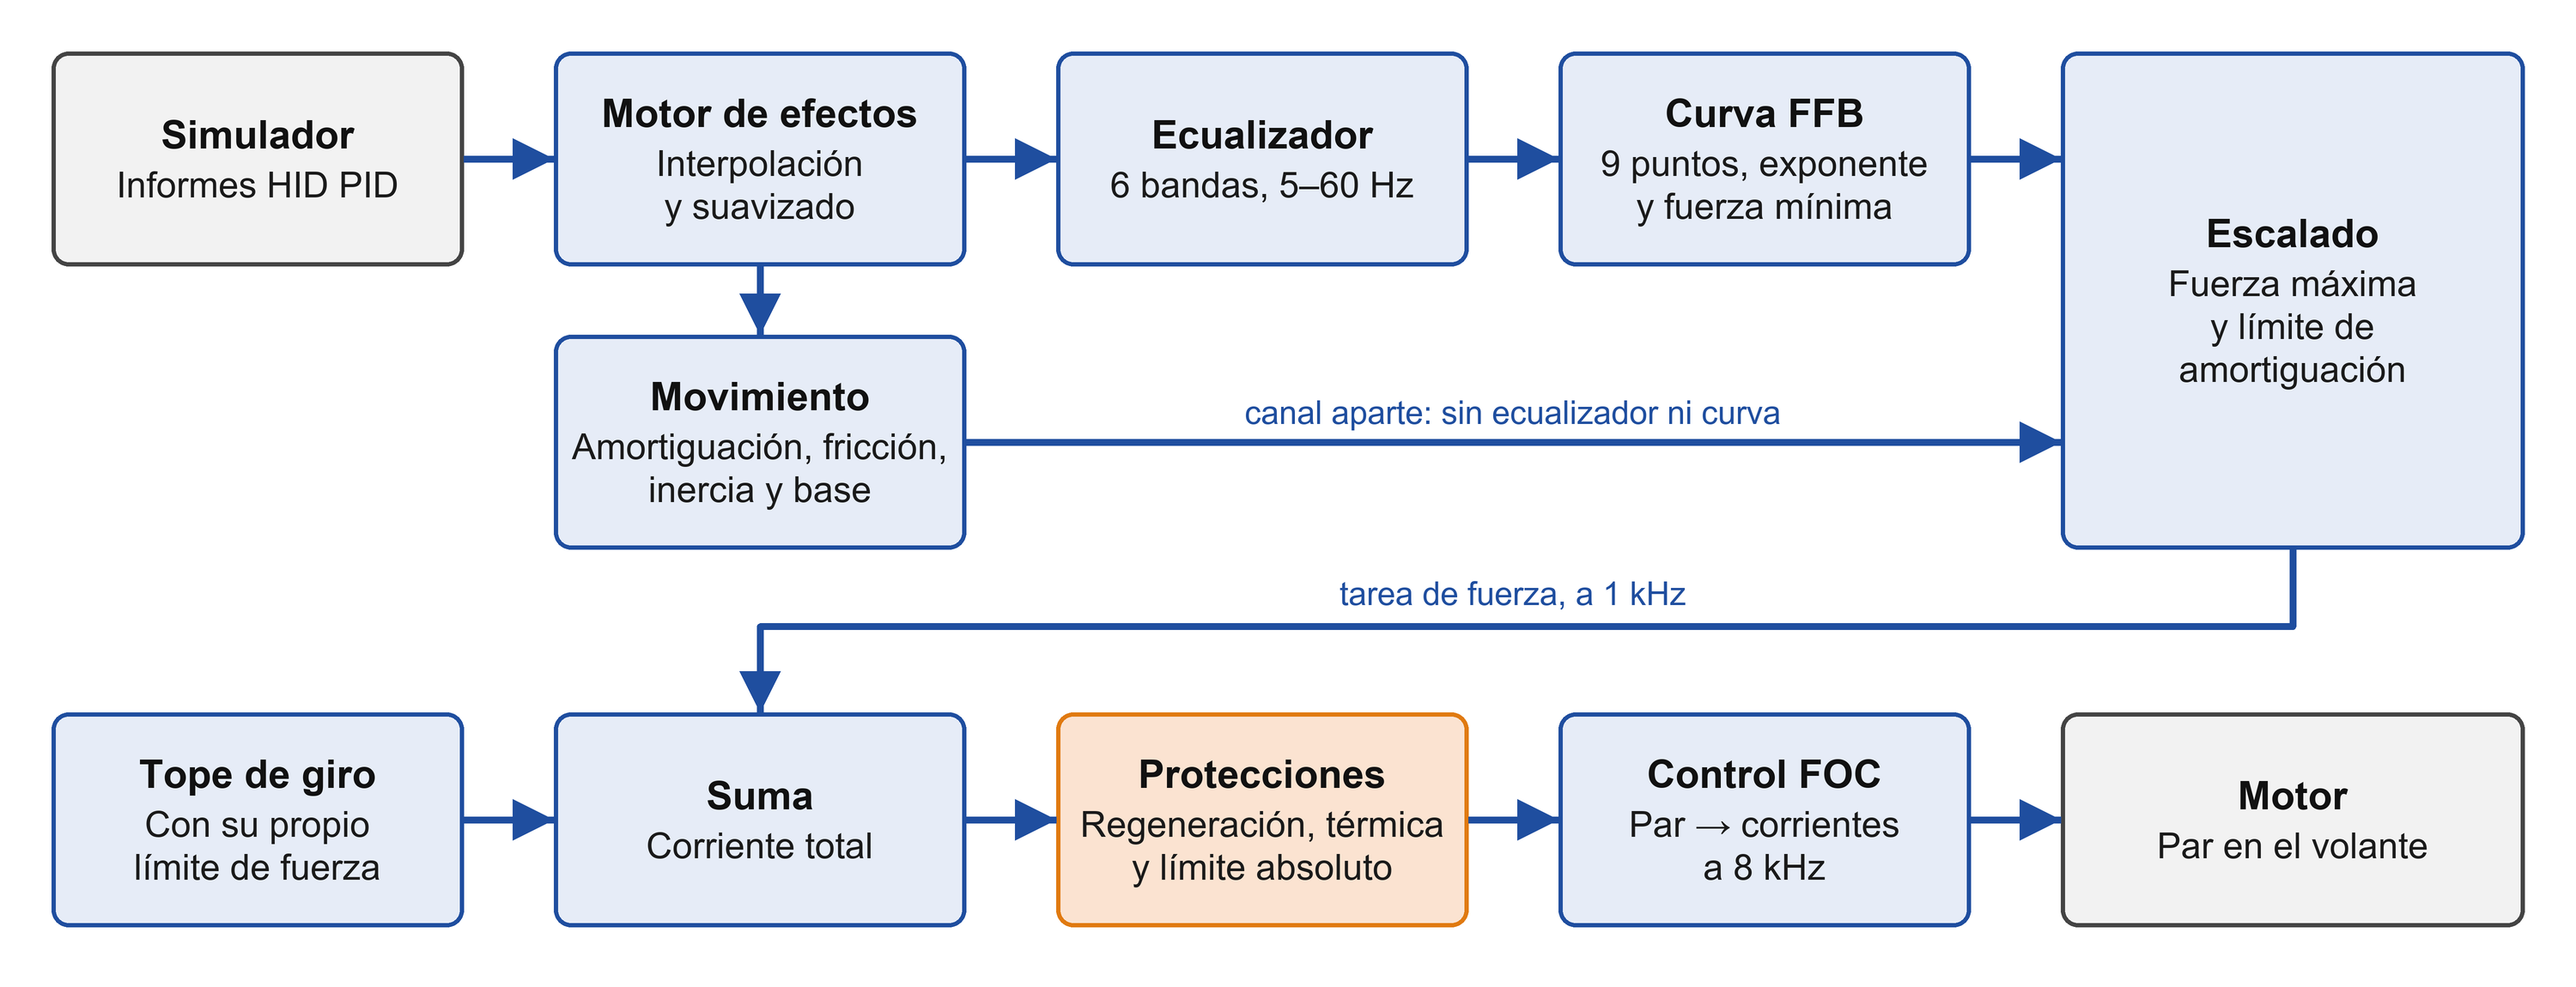
\includegraphics[width=\textwidth]{img/cadena-fuerza.png}
	\caption{Cadena de procesado de la fuerza en la base VH Grid DD15. (Fuente propia)}
	\label{fig:cadena-fuerza}
\end{figure}

Las protecciones que limitan la corriente (regeneración, térmica y límite absoluto) se sitúan al final de la cadena, justo antes del control del motor. Esta posición es una decisión deliberada: al aplicarse sobre la corriente total, sea cual sea el origen de la fuerza, ningún ajuste puede saltarse el sistema de seguridad. La vigilancia de la comunicación y el detector de oscilaciones actúan antes, sobre la fuerza que se está calculando, mientras que la sobrevelocidad y el arranque seguro gobiernan el estado del motor y cortan el par por completo. La tabla~\ref{tab:protecciones} relaciona cada protección con la magnitud que vigila y el requisito al que responde. Su funcionamiento se detalla en el apartado~\ref{subsec:fw-base}.

\begin{table}[H]
	\centering
	\caption{Protecciones de la base VH Grid DD15.}
	\label{tab:protecciones}
	\small
	\begin{tabularx}{\textwidth}{@{}>{\raggedright\arraybackslash}p{3.4cm}>{\raggedright\arraybackslash}X>{\raggedright\arraybackslash}p{1.8cm}@{}}
		\toprule
		\textbf{Protección} & \textbf{Magnitud vigilada y respuesta} & \textbf{Requisito} \\
		\midrule
		Sobrevelocidad & Velocidad del volante medida por el encoder. Limita o corta el par si supera el umbral, por ejemplo al soltar el volante con fuerza aplicada. & RNF8 \\
		Protección térmica & Calentamiento del motor, estimado a partir de la corriente acumulada (modelo I$^2$t), que reduce el par de forma progresiva. Temperatura de los transistores (termistor NTC), que reduce la corriente entre 100 y 120~\textdegree C hasta anularla. & RNF9 \\
		Tope de giro progresivo & Posición del volante respecto al rango configurado. Aplica una fuerza creciente que detiene el volante sin golpe. & RNF10 \\
		Limitador de regeneración & Tensión del bus de alimentación cuando el motor actúa como generador. Limita la energía devuelta a la fuente. & RNF11 \\
		Detector de oscilaciones & Patrón de la velocidad y la posición del volante. Amortigua o corta el par ante oscilaciones sostenidas. & RNF12 \\
		Vigilancia de la comunicación & Tiempo desde el último informe de fuerza. Lleva el par a cero si se pierde la comunicación o el juego deja de enviar fuerzas. & RNF13 \\
		Arranque seguro & Estado del motor y del encoder al encender. No aplica par hasta comprobarlos, y después lo aplica de forma gradual. & RNF14 \\
		\bottomrule
	\end{tabularx}
\end{table}

La base incorpora además una orden de mantenimiento, recibida por el canal \textit{vendor}, que la reinicia en modo de actualización. Esto permite grabar un firmware nuevo desde la aplicación sin manipular la placa (RF32), como se describe en el apartado~\ref{subsec:ux-firmware}.

\paragraph{Pedalera VH Axis y aro VH Formula Apex.}
La pedalera y el aro tienen tareas mucho más sencillas, que no justifican un sistema operativo. Su firmware se organiza como un bucle principal, con cada tarea temporizada a su propio periodo, que recorre las capas en orden, primero lee las entradas, las procesa, actualiza los informes HID y por último atiende los mensajes del puerto serie.

En la pedalera, cada vuelta del bucle lee los tres sensores a unos 1000~Hz (RNF3) y los somete a la misma secuencia que consiste en el filtrado del ruido, normalización entre los puntos de reposo y fondo de la calibración, zona muerta y curva de respuesta (RF12 y RF13). El sentido del pedal se deduce de cuál de sus dos puntos de calibración es mayor, de modo que la calibración guiada resuelve sola un sensor montado al revés, y la aplicación ofrece además una casilla que intercambia ambos puntos. El valor resultante se envía como eje del mando HID. Como toda la transformación se hace en el firmware, la pedalera entrega al simulador la respuesta configurada aunque la aplicación esté cerrada.

En el aro, el bucle escanea la matriz de pulsadores y lee los \textit{encoders} a través del expansor, y envía su estado como botones del mando HID (RF16). Los LEDs siguen un reparto de responsabilidades distinto: la decisión de qué debe mostrar cada LED depende de la telemetría y de los perfiles de luces, que solo conoce la aplicación, por lo que es esta quien calcula el estado de la tira y lo envía por el puerto serie. El aro se limita a aplicarlo con el brillo configurado, que guarda en su EEPROM para conservarlo aunque arranque sin el ordenador (RF21). Al conectarse, aro y aplicación intercambian un saludo (\textit{handshake}) que identifica al periférico y su versión de firmware antes de empezar a enviar datos.

\subsection{Aplicación}
\label{subsec:arq-aplicacion}
La aplicación VH SimGrid se desarrolla en Python para Windows 10 y 11 (RNF40). Las primeras versiones se construyeron con \textbf{Tkinter}, la biblioteca gráfica que se incluye de serie con Python. Es sencilla y no necesita instalar nada, por lo que resultó adecuada para los primeros prototipos, que solo leían y cambiaban los ajustes de los periféricos. Sin embargo, cuando la aplicación creció y pasó a incluir el \textit{dash}, las gráficas del análisis y una interfaz más cuidada, sus limitaciones en rendimiento gráfico, personalización visual y trabajo con varios hilos hicieron necesario cambiar de tecnología.

Se decidió migrar a \textbf{Qt}, un \textit{framework} de aplicaciones de escritorio mucho más completo. Frente a Tkinter, ofrece una escena gráfica que solo redibuja lo que cambia, para mantener el \textit{dash} a 30 imágenes por segundo sin sobrecargar el equipo (RNF6 y RNF7), hojas de estilo para los modos claro y oscuro, señales seguras entre hilos y soporte de varias pantallas para la pantalla del aro (RF22). La traducción de la interfaz (RNF27) se resuelve con un módulo propio, con un diccionario por idioma. A cambio, aumenta el tamaño del instalador y es más complejo de aprender, dos costes que se consideraron asumibles. La tabla~\ref{tab:tkinter-qt} resume la comparación.

\begin{table}[H]
	\centering
	\caption{Comparación entre Tkinter y Qt.}
	\label{tab:tkinter-qt}
	\small
	\begin{tabularx}{\textwidth}{@{}>{\raggedright\arraybackslash}p{3.4cm}>{\raggedright\arraybackslash}X>{\raggedright\arraybackslash}X@{}}
		\toprule
		\textbf{Criterio} & \textbf{Tkinter} & \textbf{Qt} \\
		\midrule
		Instalación y aprendizaje & Incluido en Python y muy sencillo. & Biblioteca externa y más compleja. \\
		Rendimiento gráfico & Lienzo básico. & Escena gráfica que solo redibuja lo que cambia. \\
		Personalización visual & Limitada. & Hojas de estilo para toda la aplicación. \\
		Trabajo con hilos & Sin mecanismo propio. & Señales y ranuras seguras entre hilos. \\
		Varias pantallas & Solución propia. & Soporte integrado. \\
		\bottomrule
	\end{tabularx}
\end{table}

La aplicación se organiza en tres capas: la \textbf{interfaz}, con la que interactúa el usuario; la \textbf{lógica}, que contiene toda la funcionalidad del sistema, y la \textbf{persistencia}, que guarda los datos en el disco. La figura~\ref{fig:arquitectura-app} muestra esta organización.

\begin{figure}[H]
	\centering
	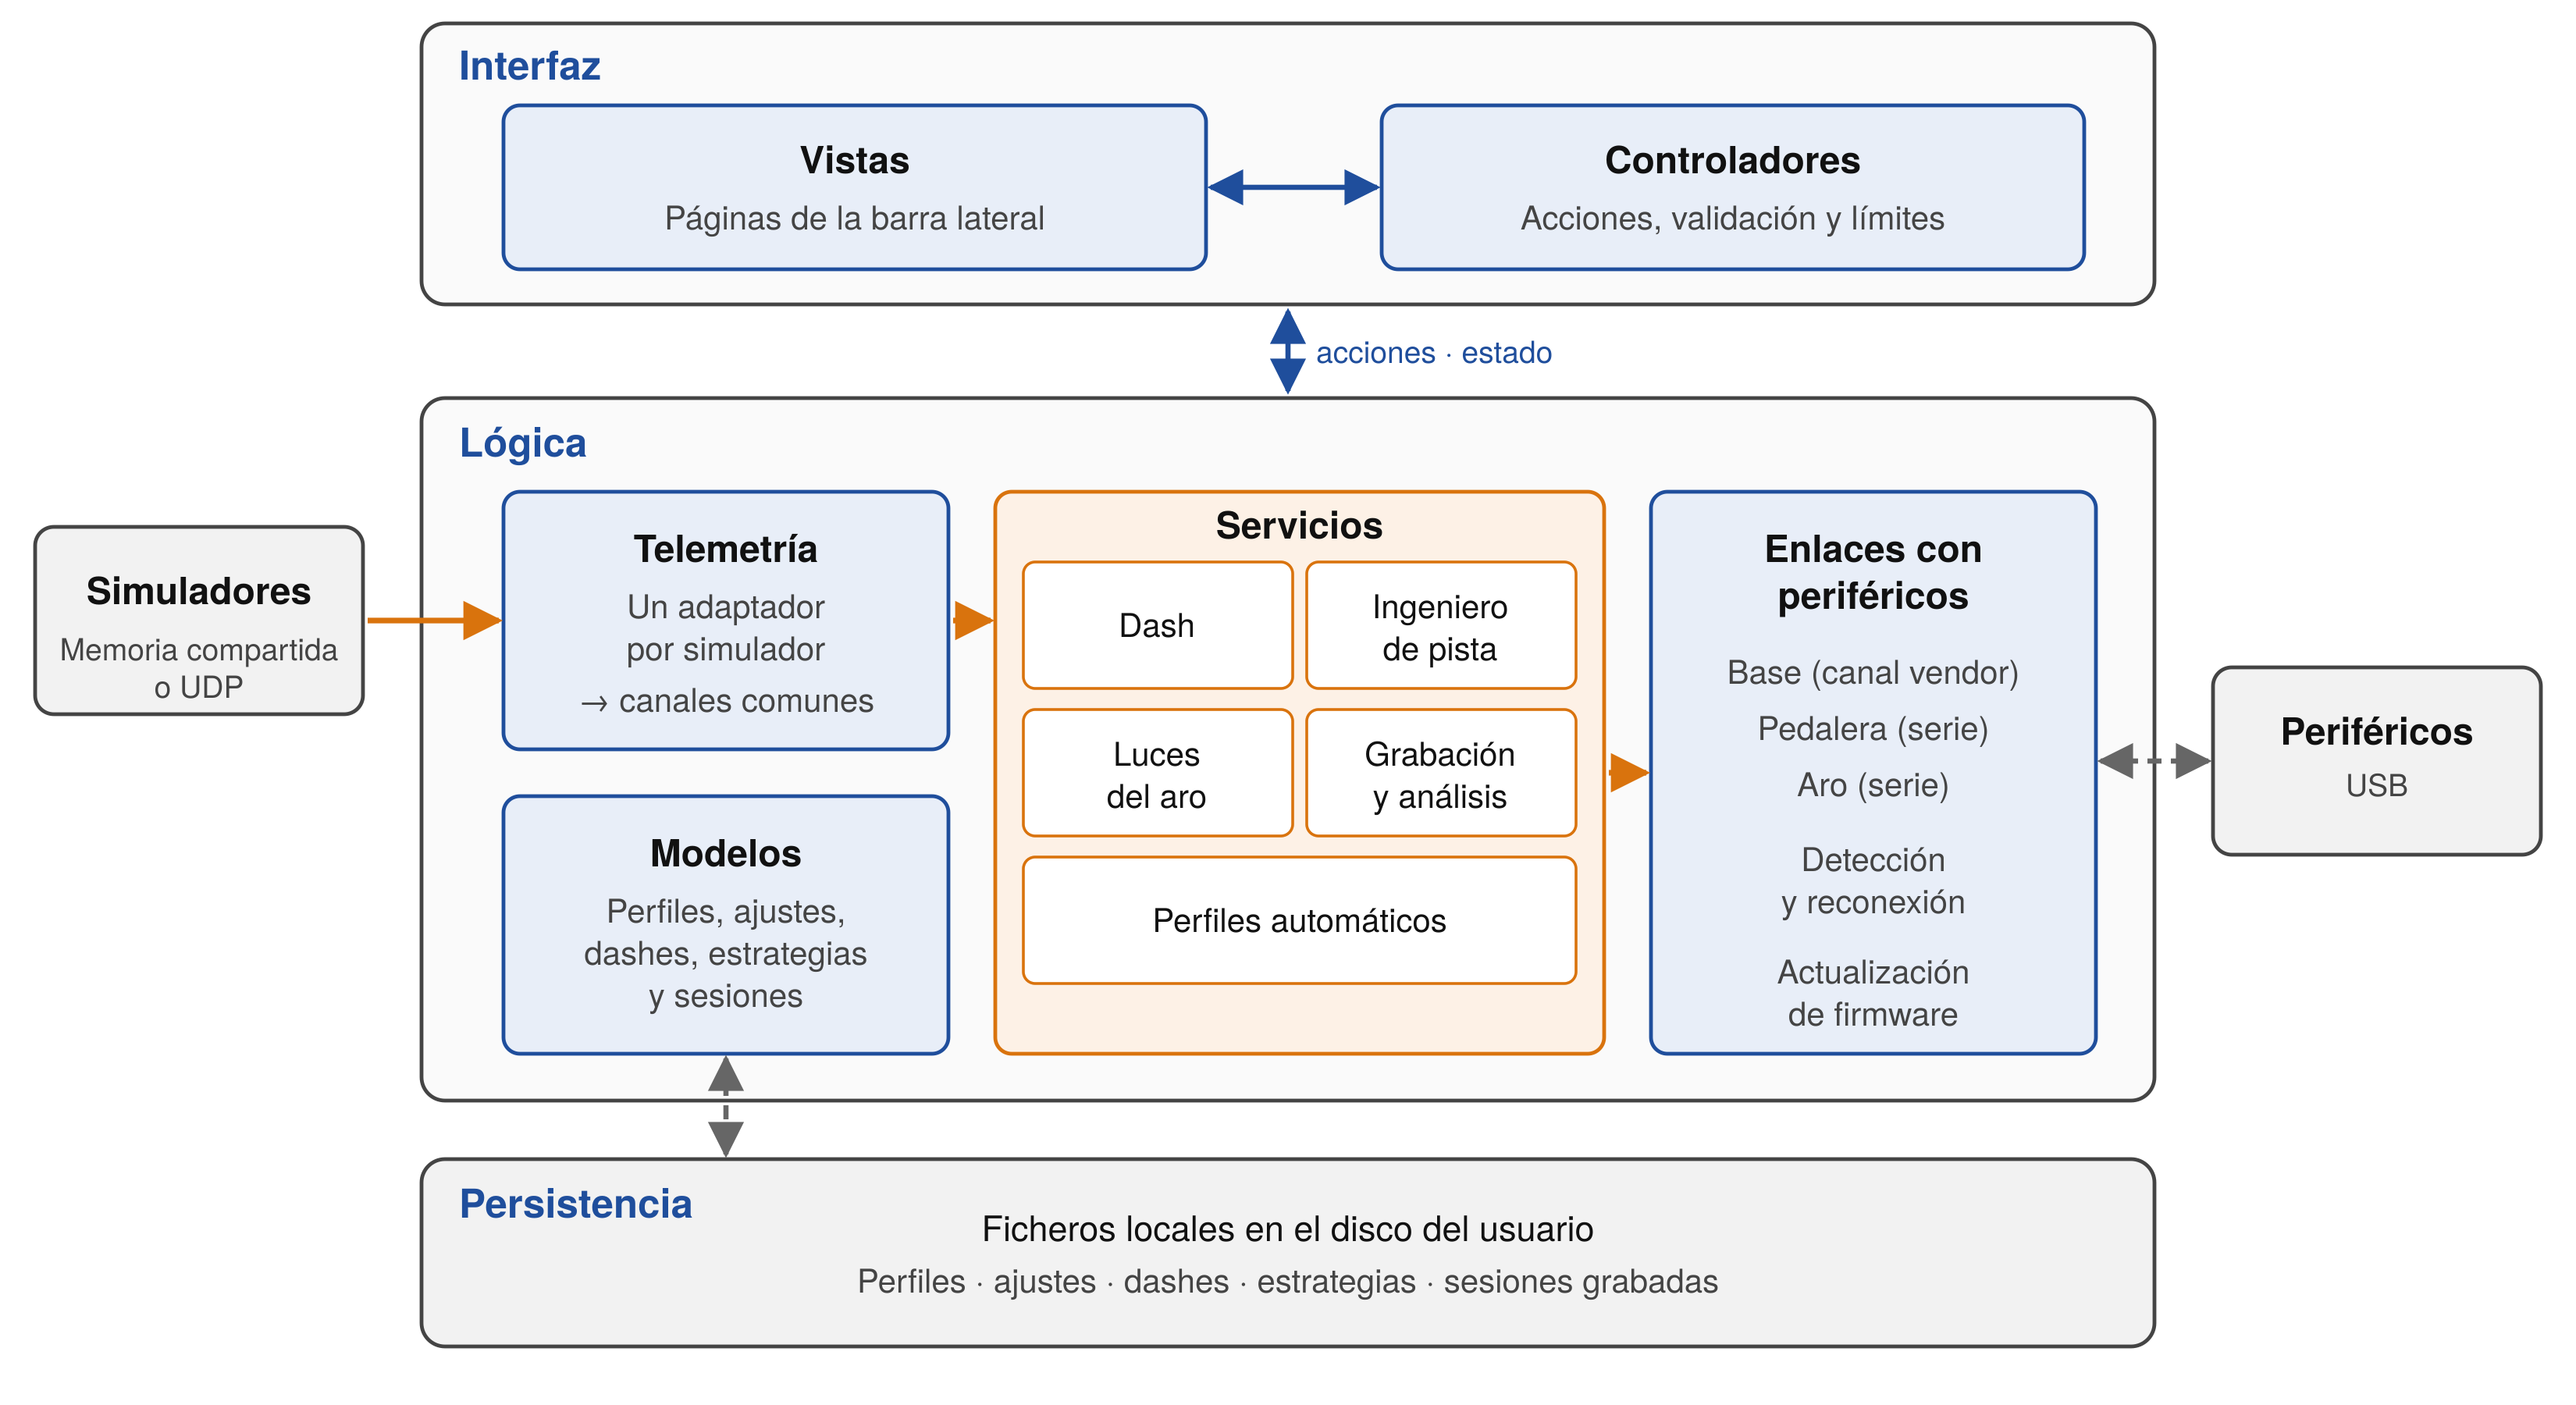
\includegraphics[width=\textwidth]{img/arquitectura-app.png}
	\caption{Arquitectura de la aplicación VH SimGrid. (Fuente propia)}
	\label{fig:arquitectura-app}
\end{figure}

\paragraph{Interfaz: vistas y controladores.}
La capa de interfaz separa lo que se muestra de lo que se hace. Las \textbf{vistas} son las páginas de la aplicación (Inicio, Volante, Aro, Pedalera, Dash, Ingeniero, Análisis y Ajustes) y solo se ocupan de presentar datos y recoger las acciones del usuario. Los \textbf{controladores} reciben esas acciones, comprueban que los valores están dentro de los límites permitidos (RNF39) y las trasladan a la capa de lógica. Las vistas nunca se comunican directamente con los periféricos ni con los simuladores, de modo que el aspecto de una página puede cambiar sin afectar al funcionamiento del sistema.

\paragraph{Lógica.}
La capa de lógica se divide en cuatro bloques:

\begin{itemize}
	\item \textbf{Modelos.} Representan en memoria los datos del sistema: los perfiles, los ajustes de cada periférico, los \textit{dashes}, las estrategias y las sesiones. Son independientes de cómo se muestran en la interfaz y de cómo se guardan en el disco.
	\item \textbf{Enlaces con periféricos.} Cada periférico tiene su propio enlace, que encapsula su protocolo: el canal \textit{vendor} de la base y el puerto serie de la pedalera y el aro. Los enlaces detectan los periféricos por su identidad USB al conectarlos y los reconectan si se pierde la conexión (RF29). Incluyen también el actualizador de firmware, que elige el fichero según el periférico conectado y comprueba la grabación al terminar (RF32 y RNF15).
	\item \textbf{Telemetría.} Cada simulador publica sus datos con su propio formato y por su propio medio, ya sea memoria compartida o paquetes UDP. Para aislar al resto de la aplicación de esta diversidad, cada simulador tiene su \textbf{adaptador}, que traduce sus datos a un conjunto común de canales (velocidad, marcha, revoluciones, posición en pista\ldots) y calcula los canales derivados que el juego no ofrece. Añadir un simulador consiste en escribir un adaptador nuevo, sin modificar nada más (RF38 y RNF43).
	\item \textbf{Servicios.} Son las funciones que consumen los canales comunes de telemetría: el \textit{dash}, que se dibuja en la pantalla del aro o en un monitor y se sirve a los móviles vinculados; el ingeniero de pista, con su motor de reglas, la síntesis de voz (Piper) y el reconocimiento de voz (Vosk); las luces del aro, que calculan el estado de la tira y lo envían por su enlace; la grabación y el análisis de sesiones, y los perfiles automáticos, que detectan el juego y el coche y aplican el perfil correspondiente. La voz y las grabaciones se procesan y guardan siempre en el propio equipo (RNF42).
\end{itemize}

Como todos los servicios trabajan sobre los mismos canales comunes, ninguno depende del simulador concreto. El mismo \textit{dash}, la misma lógica del ingeniero y las mismas hojas de análisis sirven para los 18 juegos compatibles.

\paragraph{Ejecución concurrente.}
La interfaz se ejecuta en el hilo principal, mientras que la recepción de la telemetría, los enlaces con los periféricos y el procesado de voz se ejecutan en hilos propios, que se comunican con el resto mediante colas y, en algunos casos, señales de Qt. Así, una operación lenta, como cargar una sesión grabada o reconocer una frase, nunca bloquea la interfaz, y las luces del aro se actualizan al ritmo de la telemetría con independencia de lo que se esté dibujando en pantalla (RNF4). Esta organización permite también mantener acotado el consumo de procesador mientras el simulador está en marcha (RNF7).

\paragraph{Ejemplo de funcionamiento.}
El recorrido de un cambio de ajuste muestra cómo colaboran las capas. Cuando el usuario mueve el control de la fuerza máxima en la página del volante, la vista notifica la acción a su controlador, que comprueba que el valor está dentro de los límites y actualiza el modelo del perfil activo. El enlace de la base envía el nuevo valor por el canal \textit{vendor}, y el firmware lo aplica en la copia de parámetros en RAM, con efecto inmediato. Cinco segundos después del último cambio, la aplicación le pide que lo guarde en flash. El perfil del disco solo cambia cuando el usuario lo guarda. Todo el recorrido, desde que el usuario suelta el control hasta que el motor aplica la nueva fuerza, debe completarse en menos de 200~ms (RNF5).

\section{Protocolos de comunicación}
\label{sec:protocolos}
Los protocolos de comunicación son el contrato entre las partes del sistema, es decir, fijan cómo se identifica el periférico, qué mensajes intercambia con el simulador y con la aplicación y, además, cómo se comunica la aplicación con un dispositivo móvil para reproducir el \textit{dash}.

Todos los periféricos siguen el mismo patrón, ya presentado en la sección~\ref{sec:arquitectura-tecnologica}, cada uno ofrece dos canales, uno HID estándar para el simulador y otro de configuración para la aplicación. La primera sigue especificaciones públicas y no se modifica; la segunda es propia del proyecto y es la que se describe con más detalle. Además, todas las comunicaciones de configuración siguen la misma secuencia al conectar un periférico, representada en la figura~\ref{fig:secuencia-conexion}:

\begin{enumerate}
	\item Al enchufarlo, el periférico se identifica ante Windows con su identidad USB y su nombre, y el sistema avisa a la aplicación.
	\item La aplicación le pide su modelo y su versión de firmware, y si hay una versión más reciente ofrece actualizarlo (RF32).
	\item La aplicación lee la configuración guardada en la base o en la pedalera, de modo que la interfaz muestra siempre los valores reales del dispositivo, y no una copia que podría estar desactualizada. El aro solo guarda el brillo, que le envía la aplicación.
	\item Mientras está conectado, la aplicación envía los cambios de ajuste y recibe el estado en vivo del periférico.
\end{enumerate}

\begin{figure}[H]
	\centering
	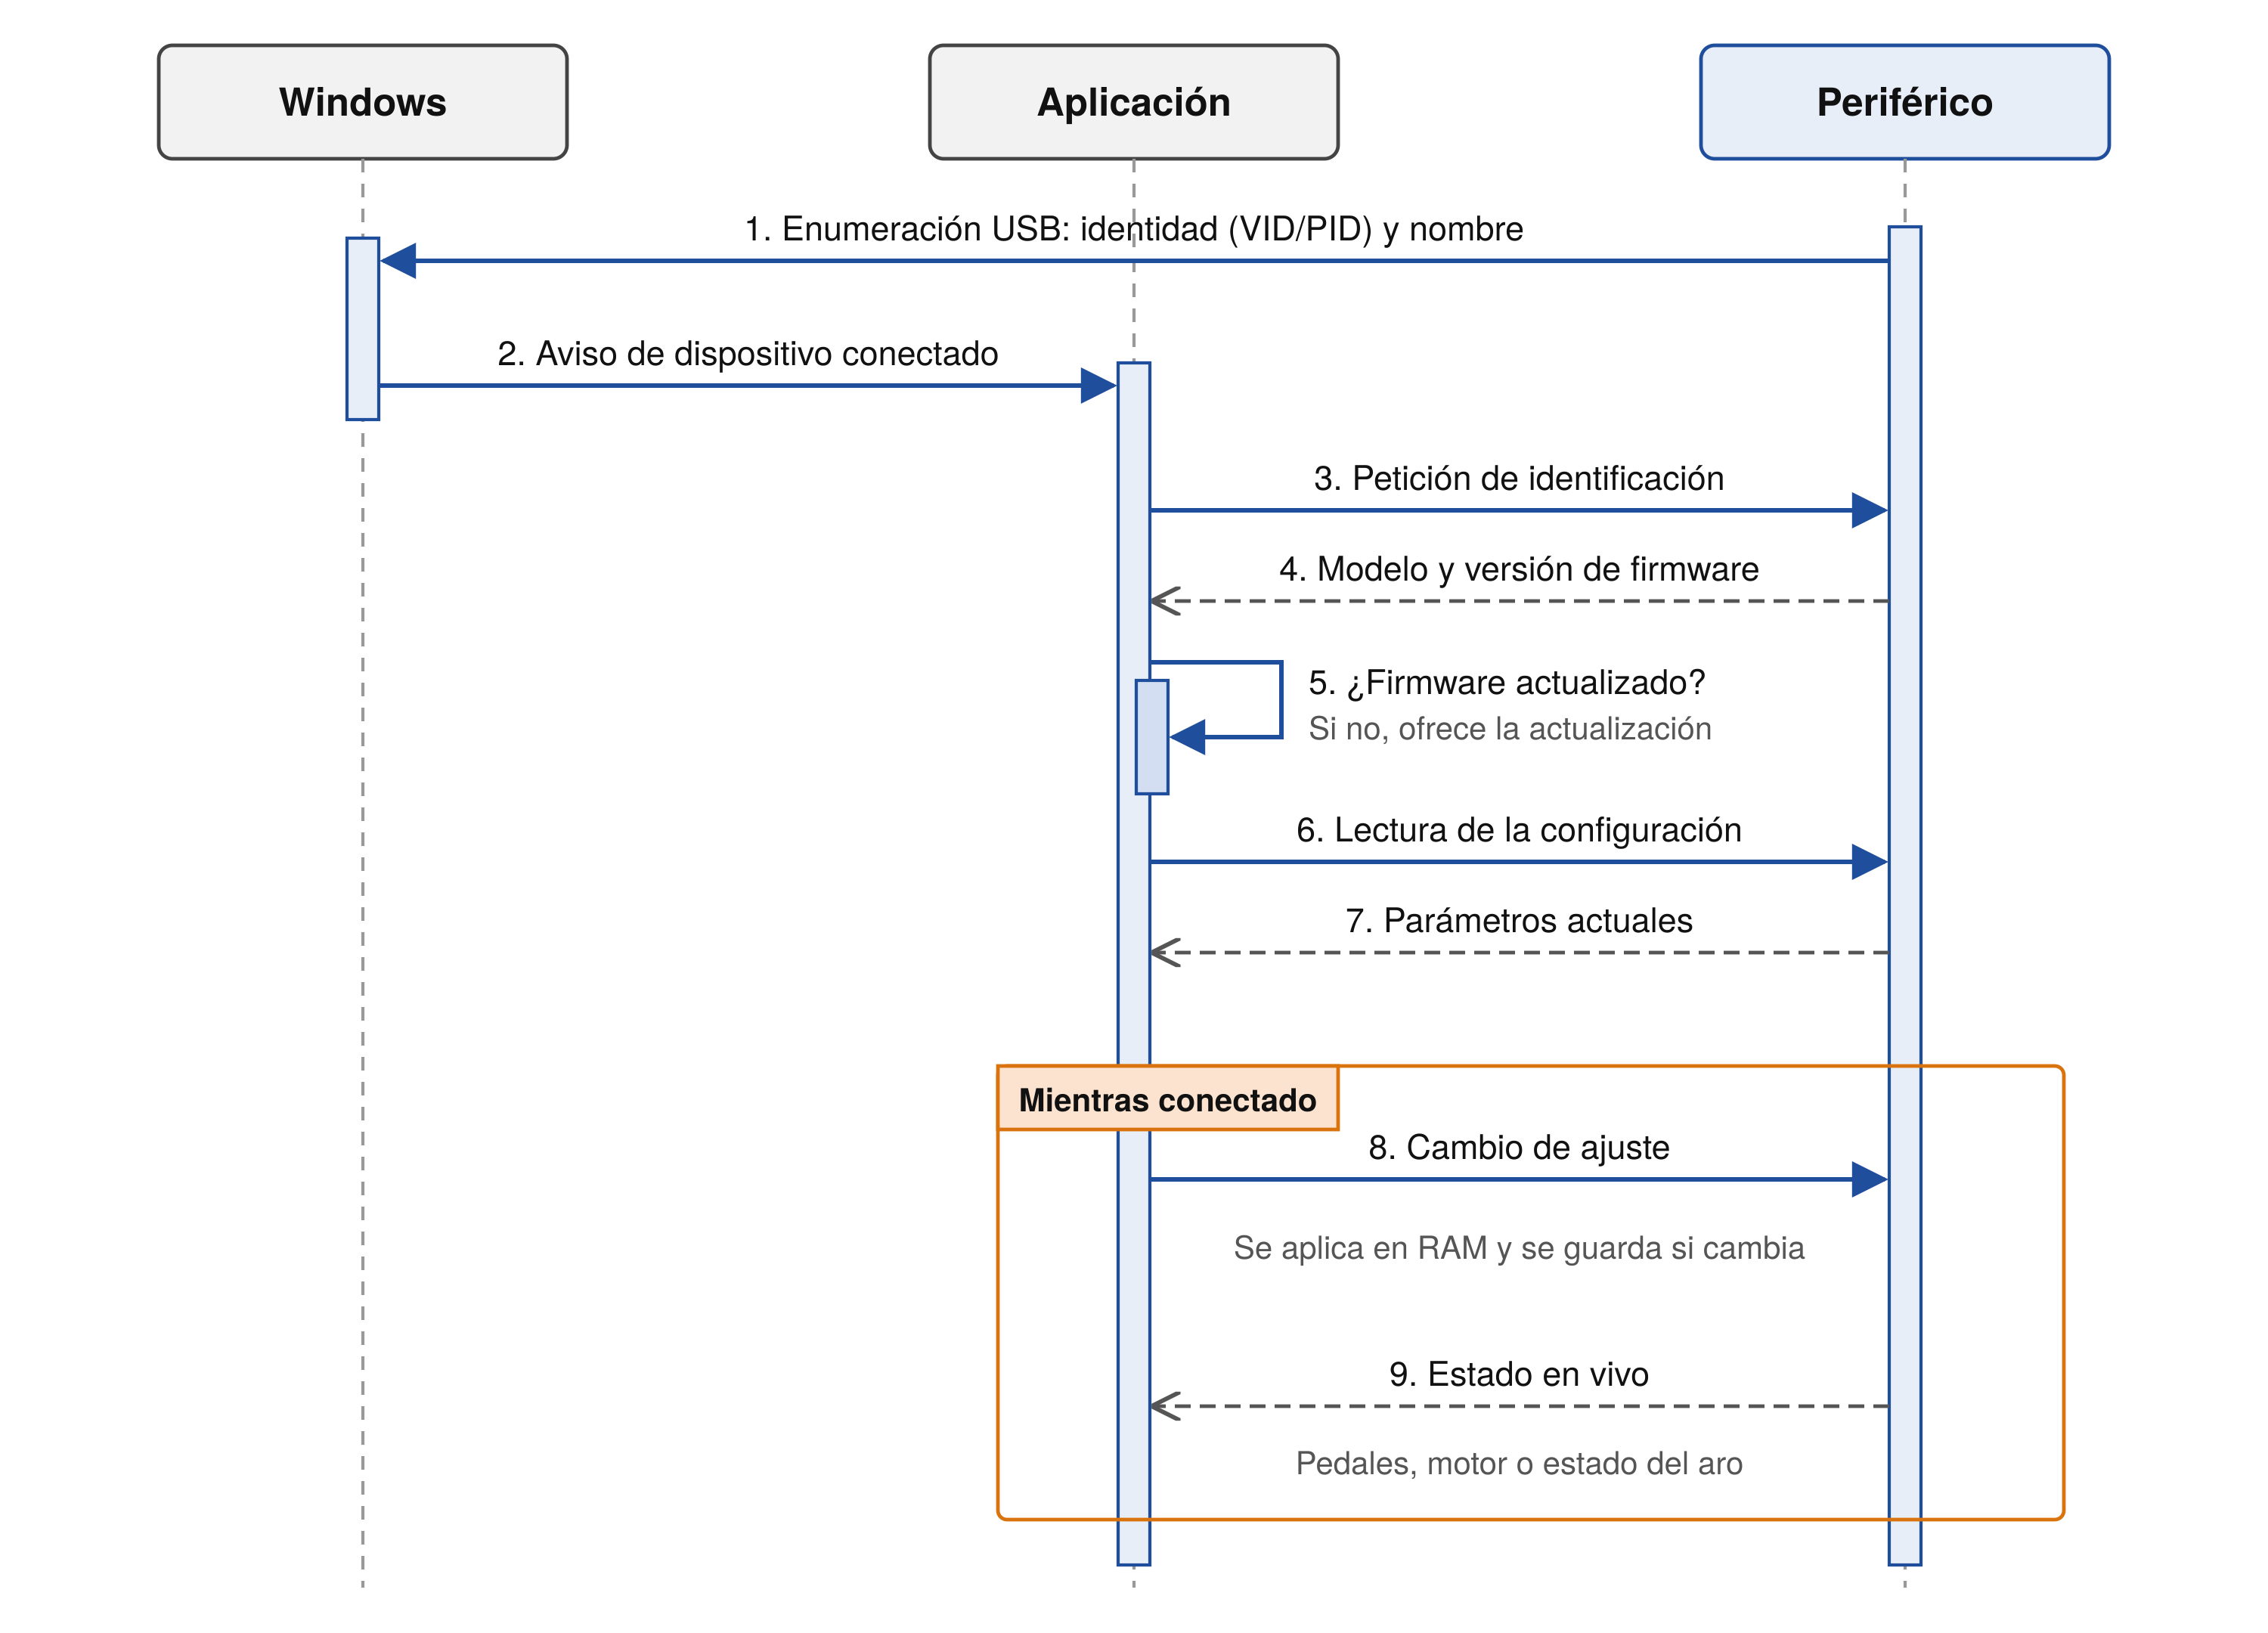
\includegraphics[width=0.9\textwidth]{img/secuencia-conexion.png}
	\caption{Secuencia de conexión entre la aplicación y un periférico. (Fuente propia)}
	\label{fig:secuencia-conexion}
\end{figure}

Leer la configuración del periférico, en lugar de imponerle la de la aplicación, es una decisión de diseño coherente con la filosofía de no depender de la aplicación para utilizar los periféricos. Solo si la base ha perdido sus ajustes, la aplicación se los devuelve a partir de la última copia que guardó.

\subsection{Identidad USB}
\label{subsec:identidad-usb}
Todo dispositivo USB se identifica con dos números de 16 bits: el identificador del fabricante (VID, \textit{Vendor ID}) y el del producto (PID, \textit{Product ID}). Junto a ellos, el dispositivo declara su nombre de producto, que es el que Windows muestra en su panel de dispositivos de juego y el que ven los simuladores al asignar los mandos.

Cada periférico tiene una identidad propia, recogida en la tabla~\ref{tab:identidad-usb}. Esta identidad cumple dos funciones. Para el usuario, los periféricos aparecen con su nombre en Windows y en los juegos, y no con un nombre genérico de la placa. Para la aplicación, es lo que permite la detección automática (RF29): al conectarse un dispositivo, la aplicación compara su VID y su PID con los de los tres periféricos y solo abre la comunicación con los que reconoce, sin confundirlos con otros mandos o placas conectados al mismo ordenador. La identidad permite además saber qué firmware corresponde a cada dispositivo antes de grabarlo (RNF15).

\begin{table}[H]
	\centering
	\caption{Identidad USB de los periféricos.}
	\label{tab:identidad-usb}
	\small
	\begin{tabularx}{\textwidth}{@{}>{\raggedright\arraybackslash}p{1.6cm}>{\raggedright\arraybackslash}p{2.8cm}>{\raggedright\arraybackslash}p{2.8cm}>{\raggedright\arraybackslash}X@{}}
		\toprule
		\textbf{Periférico} & \textbf{VID:PID} & \textbf{Nombre en Windows} & \textbf{Interfaces} \\
		\midrule
		Base & \texttt{0x1209:0xFFB1} & VH Grid DD15 & HID PID (volante con \textit{force feedback}) y canal \textit{vendor} de configuración. \\
		Pedalera & \texttt{0x2341:0x8037} & VH Axis & HID (mando de tres ejes) y puerto serie de configuración. \\
		Aro & \texttt{0x2341:0x8055} & VH Formula Apex & HID (mando de botones) y puerto serie de configuración y LEDs. \\
		\bottomrule
	\end{tabularx}
\end{table}

\subsection{Comunicación con la base}
\label{subsec:protocolo-base}
\paragraph{Interfaz HID PID.}
La comunicación con el simulador sigue la especificación HID PID (\textit{Physical Interface Device}) del USB-IF, la misma que usan los volantes comerciales, y que Windows traduce a la interfaz DirectInput de los juegos (RF1). La especificación define tres tipos de informe, que la base implementa según la tabla~\ref{tab:informes-pid}. El descriptor de la interfaz, que declara a Windows qué informes admite la base, se basa en el del proyecto abierto OpenFFBoard.

\begin{table}[H]
	\centering
	\caption{Tipos de informe HID PID que usa la base.}
	\label{tab:informes-pid}
	\small
	\begin{tabularx}{\textwidth}{@{}>{\raggedright\arraybackslash}p{2.4cm}>{\raggedright\arraybackslash}p{2.6cm}X@{}}
		\toprule
		\textbf{Tipo} & \textbf{Sentido} & \textbf{Contenido} \\
		\midrule
		Entrada & Base a simulador & Posición del volante, que el juego lee como el eje de dirección. \\
		Salida & Simulador a base & Definición y control de los efectos: crear un efecto y fijar sus parámetros (fuerza constante, muelle, amortiguación, fricción, inercia), iniciarlo o detenerlo, la ganancia global y las órdenes generales del dispositivo, como activar o desactivar los actuadores. \\
		Característica & Ambos & Reserva de memoria para un efecto nuevo y respuesta de la base indicando si lo ha podido crear. \\
		\bottomrule
	\end{tabularx}
\end{table}

La base atiende estos informes cada milisegundo (RNF1). Si dejan de llegar, porque se pierde la comunicación o el juego se cierra, la vigilancia de la comunicación lleva el par a cero (RNF13).

\paragraph{Canal \textit{vendor}.}
La configuración de la base viaja por un canal \textit{vendor}, es decir, un informe HID definido por el propio fabricante (identificador \texttt{0xA1}), dentro de la misma interfaz, que Windows no interpreta, de modo que no interfiere con los informes PID que usa el juego. El diseño del canal se basa en un modelo de \textbf{parámetros}, es decir, cada ajuste de la base (fuerza máxima, rango de giro, cada banda del ecualizador, cada punto de la curva\ldots) tiene un identificador numérico, y la aplicación los lee y escribe de uno en uno. Este modelo tiene dos ventajas, por un lado añadir un ajuste nuevo en el firmware solo requiere asignarle un identificador, sin cambiar el formato de los mensajes, y por otro lado, la aplicación puede aplicar cualquier cambio al instante, sin reenviar la configuración completa (RF30 y RNF5). La tabla~\ref{tab:canal-vendor} resume las operaciones del canal.

\begin{table}[H]
	\centering
	\caption{Operaciones del canal \textit{vendor} de la base.}
	\label{tab:canal-vendor}
	\small
	\begin{tabularx}{\textwidth}{@{}>{\raggedright\arraybackslash}p{2.8cm}>{\raggedright\arraybackslash}p{1cm}>{\raggedright\arraybackslash}p{1.6cm}X@{}}
		\toprule
		\textbf{Operación} & \textbf{Tipo} & \textbf{Código} & \textbf{Descripción} \\
		\midrule
		Identificación & \texttt{0x01} & 207 & Devuelve la versión del firmware. \\
		Leer parámetro & \texttt{0x01} & 1--35 & Devuelve el valor actual de un parámetro. \\
		Escribir parámetro & \texttt{0x02} & 1--35 & Cambia el valor de un parámetro en RAM, con efecto inmediato. El firmware ajusta a sus límites los valores que los superan y devuelve el valor aplicado (RNF39). \\
		Centrar & \texttt{0x03} & 100 & Fija la posición actual del volante como centro (RF3). \\
		Calibración anti-cogging & \texttt{0x03} & 106 & Inicia la medida del rizado magnético y guarda el resultado en flash (RF8). \\
		Estado en vivo & \texttt{0x01} & 200--206, 208--215 & Devuelve el estado y los errores del motor, la posición, la tensión de bus, la fuerza pedida, la carga térmica, la temperatura y los contadores de las protecciones, que alimentan la monitorización de la aplicación (RF9). \\
		Reinicio & \texttt{0x03} & 107 & Reinicia la base (RF10). \\
		Modo de actualización & \texttt{0x03} & 105 & Reinicia la base en el modo de grabación de firmware, sin necesidad del puente BOOT0 (RF32). \\
		\bottomrule
	\end{tabularx}
\end{table}

Todos los mensajes del canal tienen el mismo formato en los dos sentidos, recogido en la tabla~\ref{tab:formato-vendor}. Es un informe HID de 25 bytes, con los campos de varios bytes en orden \textit{little-endian}. La base responde a cada petición con el mismo mensaje, en el que marca el campo de tipo y rellena el valor. Si la petición no es válida, como ocurre con un código desconocido, lo indica en ese mismo campo.

\begin{table}[H]
	\centering
	\caption{Formato de los mensajes del canal \textit{vendor}.}
	\label{tab:formato-vendor}
	\small
	\begin{tabularx}{\textwidth}{@{}>{\raggedright\arraybackslash}p{2.8cm}>{\raggedright\arraybackslash}p{1.4cm}X@{}}
		\toprule
		\textbf{Campo} & \textbf{Bytes} & \textbf{Contenido} \\
		\midrule
		ID de informe & 1 & Siempre \texttt{0xA1}. \\
		Tipo & 1 & \texttt{0x01} leer, \texttt{0x02} escribir, \texttt{0x03} acción. La respuesta añade \texttt{0x80} y, si hay error, también \texttt{0x40}. \\
		Clase e instancia & 2 + 1 & Sin uso, a cero. Se conservan del descriptor de OpenFFBoard. \\
		Comando & 4 & Código de la operación o del parámetro. \\
		Valor & 8 & Valor leído o que se quiere escribir. \\
		Dirección & 8 & Sin uso, a cero. \\
		\bottomrule
	\end{tabularx}
\end{table}

\subsection{Comunicación con la pedalera y el aro}
\label{subsec:protocolo-pedalera-aro}
La pedalera y el aro se presentan ante el simulador como mandos HID estándar, la pedalera con tres ejes (RF11) y el aro con sus botones (RF16). Estos informes los define la propia especificación HID, sin ninguna extensión, por lo que cualquier juego los reconoce.

Para la configuración, ambos usan un \textbf{puerto serie virtual} sobre USB, que Windows reconoce como un puerto COM sin necesidad de controladores. Se eligió el puerto serie porque es la forma más sencilla de comunicarse con un ATmega32U4 y porque permite enviar mensajes en ambos sentidos en cualquier momento, lo que la pedalera necesita para la traza en vivo y el aro para recibir el estado de los LEDs. Los dos periféricos comparten el mismo esquema de mensajes, basado en órdenes de la aplicación y respuestas del periférico, y se diferencian en las operaciones que admiten, recogidas en la tabla~\ref{tab:comandos-serie}.

\begin{table}[H]
	\centering
	\caption{Operaciones del canal serie de la pedalera y el aro.}
	\label{tab:comandos-serie}
	\small
	\begin{tabularx}{\textwidth}{@{}>{\raggedright\arraybackslash}p{2.4cm}>{\raggedright\arraybackslash}p{1.5cm}>{\raggedright\arraybackslash}p{3.6cm}X@{}}
		\toprule
		\textbf{Operación} & \textbf{Periférico} & \textbf{Mensaje} & \textbf{Descripción} \\
		\midrule
		Identificación & Ambos & \texttt{VER} (pedalera), \texttt{PING} (aro) & Saludo inicial (\textit{handshake}): el periférico devuelve su modelo y su versión de firmware. \\
		Leer configuración & Pedalera & \texttt{GETCAL} & Devuelve los ajustes activos en una línea \texttt{CALDATA}. \\
		Escribir ajustes & Pedalera & \texttt{CAL,<30 valores>} & Cambia los 30 ajustes a la vez: reposo, fondo, zona muerta y 7 puntos de curva por pedal. Los aplica al momento, guarda en EEPROM solo lo que ha cambiado y responde \texttt{CALOK} o \texttt{CALERR} (RF14 y RNF22). \\
		Calibrar & Pedalera & \texttt{CAL,<30 valores>} & La aplicación toma de la traza la lectura de un pedal como su posición de reposo o de fondo, y la envía con este mensaje (RF12). \\
		Traza en vivo & Pedalera & \texttt{<a>,<e>,<f>} y \texttt{FINE,<a>,<e>,<f>} & Con el puerto abierto, envía cada 20~ms la lectura del acelerador, el embrague y el freno para la gráfica de la aplicación (RF15). \\
		Estado de los LEDs & Aro & \texttt{FRAME,<rrggbb...>} & Fija el color de cada LED de la tira, a partir de la telemetría que procesa la aplicación (RF18 y RF19). \\
		Brillo & Aro & \texttt{BRIGHT,<0-255>} & Fija el brillo de la tira y lo guarda para conservarlo sin el ordenador (RF21). \\
		Modo de actualización & Ambos & Sin mensaje: abrir el puerto a 1200 baudios & Reinicia el periférico en su cargador de arranque para grabar un firmware nuevo (RF32). \\
		\bottomrule
	\end{tabularx}
\end{table}

A diferencia del canal binario de la base, estos mensajes son líneas de texto ASCII terminadas en un salto de línea, con los campos separados por comas, de modo que se pueden leer y probar con cualquier monitor serie. La primera palabra indica la operación, salvo en la traza, que solo contiene números. En \texttt{FRAME}, cada LED ocupa seis caracteres hexadecimales.

El mensaje del estado de los LEDs es el único que se envía de forma continua durante la conducción. Para que la tira refleje un cambio de la telemetría en menos de 50~ms (RNF4), la aplicación lo envía cada 30~ms, y el aro lo aplica en cuanto lo recibe.

\subsection{Dash en dispositivos móviles}
\label{subsec:protocolo-movil}
El \textit{dash} puede mostrarse en un teléfono móvil conectado a la misma red local que el ordenador (RF41). Para no obligar al usuario a instalar nada en el móvil, la aplicación incluye un \textbf{servidor web local} y el \textit{dash} se abre en el navegador del teléfono. La vinculación se hace con un código QR, que evita tener que escribir a mano la dirección del ordenador en la red. La figura~\ref{fig:secuencia-movil} muestra el proceso:

\begin{enumerate}
	\item Cuando el piloto pide vincular un móvil, la aplicación pone en marcha el servidor y genera un código QR con su dirección en la red local y un código de invitación.
	\item El piloto escanea el código con la cámara del móvil, que abre esa dirección en el navegador.
	\item El móvil se da de alta con esa invitación y recibe su propio código de acceso, de modo que se le puede retirar el acceso sin afectar a los demás.
	\item Mientras el móvil está conectado, la aplicación dibuja el \textit{dash} elegido a la medida de su pantalla y le envía las imágenes en un flujo MJPEG, de hasta 20 imágenes por segundo, que el navegador muestra.
\end{enumerate}

\begin{figure}[H]
	\centering
	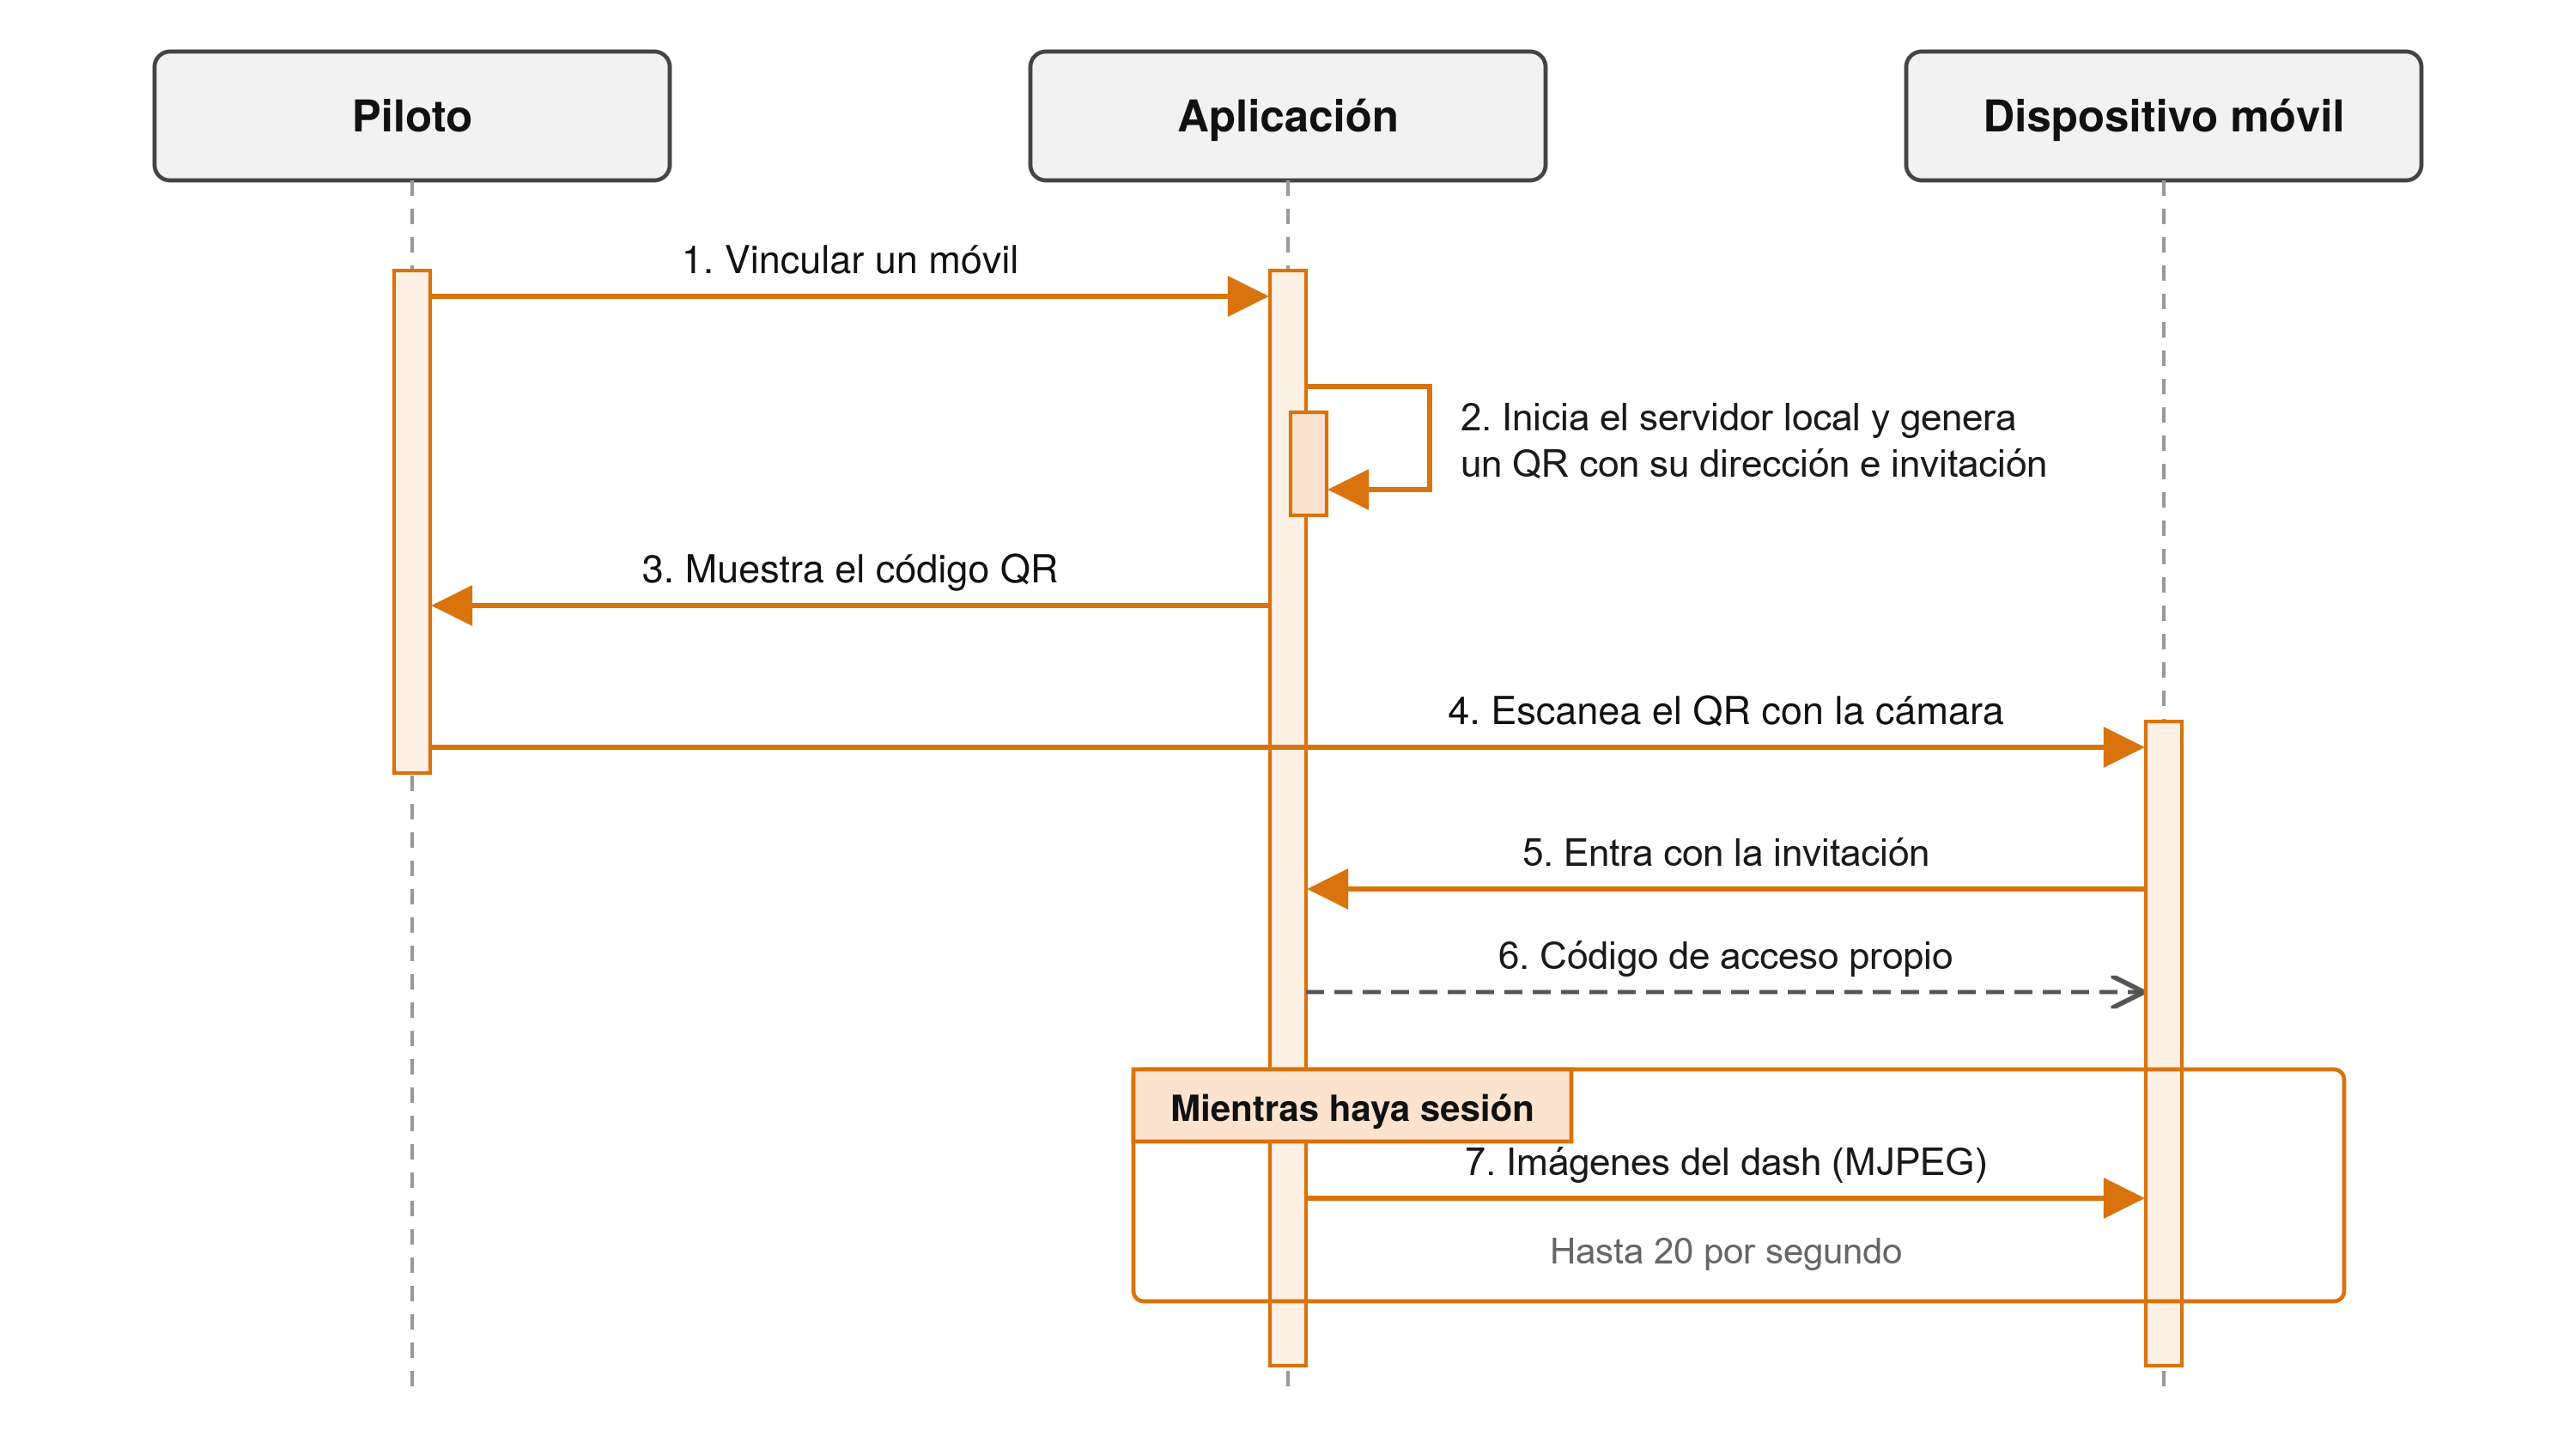
\includegraphics[width=0.9\textwidth]{img/secuencia-movil.png}
	\caption{Secuencia de vinculación y envío del \textit{dash} a un dispositivo móvil. (Fuente propia)}
	\label{fig:secuencia-movil}
\end{figure}

Dibujar el \textit{dash} en el ordenador y enviar las imágenes ya hechas evita tener que rehacer su motor de dibujo en el navegador: el móvil solo necesita una página mínima y muestra lo mismo que la pantalla del aro. A cambio, el tráfico es mayor que si se enviaran solo los valores, por lo que la aplicación ajusta las imágenes a un límite de ancho de banda y, si la red va lenta, descarta las que no llegan a tiempo en lugar de acumular retraso. Toda la comunicación se mantiene dentro de la red local, sin pasar por ningún servidor externo, de acuerdo con el requisito de privacidad RNF42.

\section{Diseño de la persistencia}
\label{sec:persistencia}
El sistema guarda sus datos en dos niveles. Cada \textbf{periférico} guarda en su propia memoria no volátil la configuración con la que funciona en ese momento, de modo que la conserva al desconectarlo y puede usarse sin la aplicación (RNF19 y RNF20). La \textbf{aplicación} guarda en el disco del ordenador todo lo demás: la biblioteca de perfiles entre los que el usuario puede elegir, sus propios ajustes, los \textit{dashes}, las estrategias y las sesiones grabadas.

La relación entre ambos niveles es sencilla: el periférico guarda una sola configuración, la activa, y la aplicación guarda todas las posibles. Cuando el usuario elige un perfil, o la aplicación lo aplica de forma automática al detectar el juego (RF31), la aplicación escribe sus valores en el periférico, que pasan a ser su nueva configuración activa. Esta sección describe qué se guarda en cada nivel, dónde y cuándo.

\subsection{Periféricos}
\label{subsec:persistencia-perifericos}
La base guarda sus datos en la memoria flash del STM32F405, y la pedalera y el aro, en la EEPROM de su ATmega32U4. La tabla~\ref{tab:persistencia-perifericos} recoge el contenido de cada una.

\begin{table}[H]
	\centering
	\caption{Datos guardados en la memoria de cada periférico.}
	\label{tab:persistencia-perifericos}
	\small
	\begin{tabularx}{\textwidth}{@{}>{\raggedright\arraybackslash}p{2.4cm}>{\raggedright\arraybackslash}p{1.8cm}X>{\raggedright\arraybackslash}p{3.2cm}@{}}
		\toprule
		\textbf{Periférico} & \textbf{Memoria} & \textbf{Datos} & \textbf{Cuándo se escribe} \\
		\midrule
		Base VH Grid DD15 & Flash & Ajustes del \textit{force feedback}: rango de giro, fuerza máxima, suavizado, tope, efectos base, ecualizador y curva. & Cinco segundos después del último cambio y al cerrar la aplicación. \\
		& & Configuración del motor y del encoder. & Junto con los ajustes. \\
		& & Tabla de compensación anti-cogging. & Al terminar la calibración. \\
		Pedalera VH Axis & EEPROM & Por cada pedal: reposo, fondo, zona muerta y los siete puntos de la curva de respuesta. & Al cambiar un ajuste o calibrar. \\
		Aro VH Formula Apex & EEPROM & Brillo de la tira. & Al cambiar el brillo. \\
		\bottomrule
	\end{tabularx}
\end{table}

La posición del centro del volante no se conserva entre sesiones, esto es debido a que el encoder es incremental, la base no conoce su posición absoluta al arrancar y toma como centro la posición en la que se enciende. En la pedalera, la inversión de un pedal no necesita un dato propio, porque se deduce de cuál de sus dos valores, reposo o fondo, es mayor.

En el aro no se guarda la asignación de luces por eventos ni los umbrales de revoluciones, porque solo tienen sentido con la telemetría y, por tanto, con la aplicación abierta. Tampoco el modo y el punto de mordida de las palancas de embrague. Todos ellos los guarda la aplicación (apartado~\ref{subsec:persistencia-aplicacion}).

El diseño de la persistencia en los periféricos responde a tres criterios:

\begin{itemize}
	\item \textbf{Proteger los ciclos de escritura.} Tanto la flash como la EEPROM admiten un número limitado de escrituras antes de degradarse, del orden de diez mil en la flash del STM32F405 y de cien mil en la EEPROM del ATmega32U4. Como un control deslizante de la aplicación puede enviar decenas de cambios en pocos segundos, cada cambio se aplica de inmediato en la copia de RAM, y la escritura en la memoria no volátil se limita de dos formas. En la EEPROM solo se escriben los bytes que realmente han cambiado (RNF22). En la flash, que se borra por sectores completos, la aplicación agrupa los cambios y pide guardar la configuración cinco segundos después del último. El bloque nuevo se añade a continuación del anterior, y un sector solo se borra cuando ya no queda sitio.
	\item \textbf{Separar los datos del programa.} En la base, la configuración y la tabla anti-cogging ocupan los dos últimos sectores de la flash, de 128~kB cada uno, reservados y distintos de los 768~kB del firmware. Así, al grabar una versión nueva solo se reescribe la zona del programa y se conserva la calibración, que de otro modo habría que repetir tras cada actualización (RNF24).
	\item \textbf{Arrancar siempre con datos válidos.} Los datos guardados llevan una marca que el firmware comprueba al arrancar, antes de usarlos. En la base es una suma de comprobación CRC-16 de toda la configuración, calculada junto con la versión de su formato, y en la pedalera y el aro, un valor fijo que identifica los datos. Si la comprobación falla, como en un periférico recién montado o, en la base, con datos dañados o de un formato incompatible, se cargan unos valores por defecto seguros en lugar de unos valores desconocidos, lo que en la base forma parte del arranque seguro (RNF14). Antes de recurrir a ellos, la base intenta leer los datos con el formato anterior, para que una actualización que cambie la estructura no pierda los ajustes ni la tabla anti-cogging.
\end{itemize}

\subsection{Aplicación}
\label{subsec:persistencia-aplicacion}
La aplicación guarda sus datos en ficheros junto al ejecutable, porque el programa se instala dentro de la carpeta de datos locales del usuario de Windows, en la ruta \texttt{\%LOCALAPPDATA\%\textbackslash\allowbreak{}VH~SimGrid\textbackslash\allowbreak{}ui\textbackslash\allowbreak{}configurador}. Esta ubicación tiene dos consecuencias. Por un lado, la aplicación se instala y escribe sus datos sin permisos de administrador (RNF25). Por otro, aunque programa y datos comparten carpeta, una actualización sustituye los ficheros del programa y el instalador no sobrescribe los perfiles y \textit{dashes} que ya existen ni toca los ajustes o las grabaciones, de modo que se conservan (RNF24). Todos los datos se quedan en el disco del usuario, sin enviarse a ningún servicio externo (RNF42). La tabla~\ref{tab:persistencia-aplicacion} resume lo que se guarda.

\begin{table}[H]
	\centering
	\caption{Datos guardados por la aplicación.}
	\label{tab:persistencia-aplicacion}
	\small
	\begin{tabularx}{\textwidth}{@{}>{\raggedright\arraybackslash}p{2.1cm}>{\raggedright\arraybackslash}p{4.4cm}X@{}}
		\toprule
		\textbf{Datos} & \textbf{Ubicación} & \textbf{Contenido} \\
		\midrule
		Ajustes de la aplicación & \texttt{ajustes.json} & Idioma, tema, arranque con Windows, segundo plano, reconexión automática, límite de grabaciones y configuración de voz y de avisos del ingeniero (RF36, RF45 y RF48). \\
		Perfiles & \texttt{perfiles/volante/}, \texttt{perfiles/pedales/}, \texttt{perfiles/aro/} & Un fichero por perfil y periférico. El del aro incluye la asignación de luces, el brillo y los ajustes de las palancas de embrague. En los ajustes se anota qué perfil de volante corresponde a cada juego y coche, y qué perfil de aro a cada juego (RF20 y RF31). \\
		\textit{Dashes} & \texttt{perfiles/dash/\allowbreak{}<nombre>/} & Diseño de cada \textit{dash} en \texttt{dash.json} (pantallas, elementos, propiedades y fórmulas), junto a sus imágenes y fuentes. Los 20 de serie se instalan en esta misma carpeta (RF40 y RF42). \\
		Estrategias & \texttt{perfiles/\allowbreak{}strategies/\allowbreak{}library.json} & Estrategias de carrera guardadas por juego, coche y circuito, con los datos de la carrera y las paradas (RF50 y RF52). \\
		Historial & \texttt{perfiles/sessions/}, \texttt{perfiles/references/}, \texttt{perfiles/mapas/} & Fichas por vuelta de cada sesión, vueltas de referencia y mapas de pista. \\
		Sesiones grabadas & \texttt{grabaciones/} & Telemetría cruda de cada sesión, con todos sus canales, y el índice de la lista de sesiones (RF53). \\
		\bottomrule
	\end{tabularx}
\end{table}

Se distinguen dos tipos de datos según su tamaño y su uso:

\begin{itemize}
	\item \textbf{Datos de configuración e historial}: todo salvo las grabaciones. Son pequeños y el usuario los modifica a menudo, por lo que se guardan en JSON, un formato de texto fácil de leer y de depurar. Se escriben primero en un fichero temporal, que después sustituye al definitivo de una sola vez, para que un corte de luz a mitad no deje un fichero dañado. Los \textit{dashes}, las estrategias y las fichas de sesión indican además la versión de su formato, y los perfiles combinados de versiones antiguas se convierten solos al arrancar.
	\item \textbf{Sesiones grabadas}: cada una contiene miles de muestras de cientos de canales, tomadas a 30~Hz, por lo que se guardan en texto JSON comprimido con gzip (\texttt{.jsonl.gz}). Cada línea es un instante y solo recoge los canales que han cambiado, lo que reduce mucho su tamaño. Para que el disco no se llene, la aplicación conserva un número máximo de grabaciones, 20 de fábrica y configurable por el usuario, además de un límite opcional de espacio, y borra las más antiguas al superarlo (RF53). La primera línea de cada grabación es una cabecera con el juego, el coche y el circuito, y el mejor tiempo se calcula una vez y se guarda en \texttt{indice.json}, lo que permite mostrar y filtrar la lista de sesiones sin abrir cada grabación (RF54).
\end{itemize}

Por último, la aplicación permite reunir sus datos en un solo fichero \texttt{.zip} de copia de seguridad, que el usuario puede guardar o llevar a otro ordenador y restaurar después (RF35). La copia incluye también las sesiones grabadas, porque son lo único que no se puede volver a generar, y deja fuera solo el certificado del dispositivo móvil, que lleva una clave privada y se crea de nuevo en cada equipo. Los \textit{dashes} pueden además exportarse e importarse de uno en uno en un fichero comprimido \texttt{.vhdash.zip}, para compartirlos con otros usuarios (RF43).

\section{Experiencia de usuario (UX)}
\label{sec:ux}
El usuario objetivo de VH SimGrid es un piloto aficionado, no un tecnico (tabla~\ref{tab:actores}). Debe poder utilizar, calibrar y poner en marcha el equipo sin necesidad de tener conocimientos de programación o electronica (RNF26). Por eso la experiencia de usuario no se limita al aspecto de las pantallas, que se trata en la sección~\ref{sec:ui}, sino que abarca cómo se desarrollan los pasos que tiene cada una, en qué orden, qué ve el piloto en cada momento y qué ocurre cuando algo sale mal.

El diseño de la interacción se apoya en las heurísticas de usabilidad de Nielsen~\cite{nielsen1994}, adaptadas al contexto del simracing. La tabla~\ref{tab:principios-ux} recoge los principios aplicados y cómo se reflejan en el sistema.

\begin{table}[H]
	\centering
	\caption{Principios de experiencia de usuario aplicados en VH SimGrid.}
	\label{tab:principios-ux}
	\small
	\begin{tabularx}{\textwidth}{@{}>{\raggedright\arraybackslash}p{3.6cm}X@{}}
		\toprule
		\textbf{Principio} & \textbf{Aplicación en el sistema} \\
		\midrule
		Funcionar al conectar & Los periféricos se detectan y se configuran solos, y la aplicación lee su estado real en lugar de pedírselo al usuario (RF29). \\
		Visibilidad del estado & Cada acción tiene una respuesta visible: la traza en vivo de los pedales, la vista previa de los LEDs, el estado de cada periférico o el perfil activo (RNF28). \\
		Guiar en lugar de configurar & Las tareas con varios pasos, como la puesta en marcha o la calibración, se resuelven con asistentes que piden una sola acción cada vez. \\
		Lenguaje del piloto & Los valores se expresan en las unidades que entiende el piloto, como los kilos en el freno o los grados de giro, y no en lecturas del sensor. \\
		Prevención de errores & Los valores fuera de rango se limitan, el firmware se comprueba antes de grabarlo y las lecturas dudosas se repiten (RNF15 y RNF39). \\
		Control del usuario & Toda tarea guiada puede posponerse o cerrarse y reanudarse después, y toda decisión automática puede cambiarse a mano. \\
		Sin soltar el volante & Lo que se necesita durante la conducción se maneja con los mandos del aro o por voz (RNF29). \\
		\bottomrule
	\end{tabularx}
\end{table}

Los apartados siguientes describen los cuatro flujos en los que estos principios tienen más peso. Cada uno se representa con un diagrama de flujo y se corresponde con un caso de uso del capítulo~\ref{cap:requisitos}.

\subsection{Primera configuración}
\label{subsec:ux-asistente}
La primera vez que se abre la aplicación, un asistente guía al piloto por la puesta en marcha completa del equipo (RF33), siguiendo el caso de uso CU1. Su flujo se muestra en la figura~\ref{fig:ux-asistente}.

\begin{figure}[H]
	\centering
	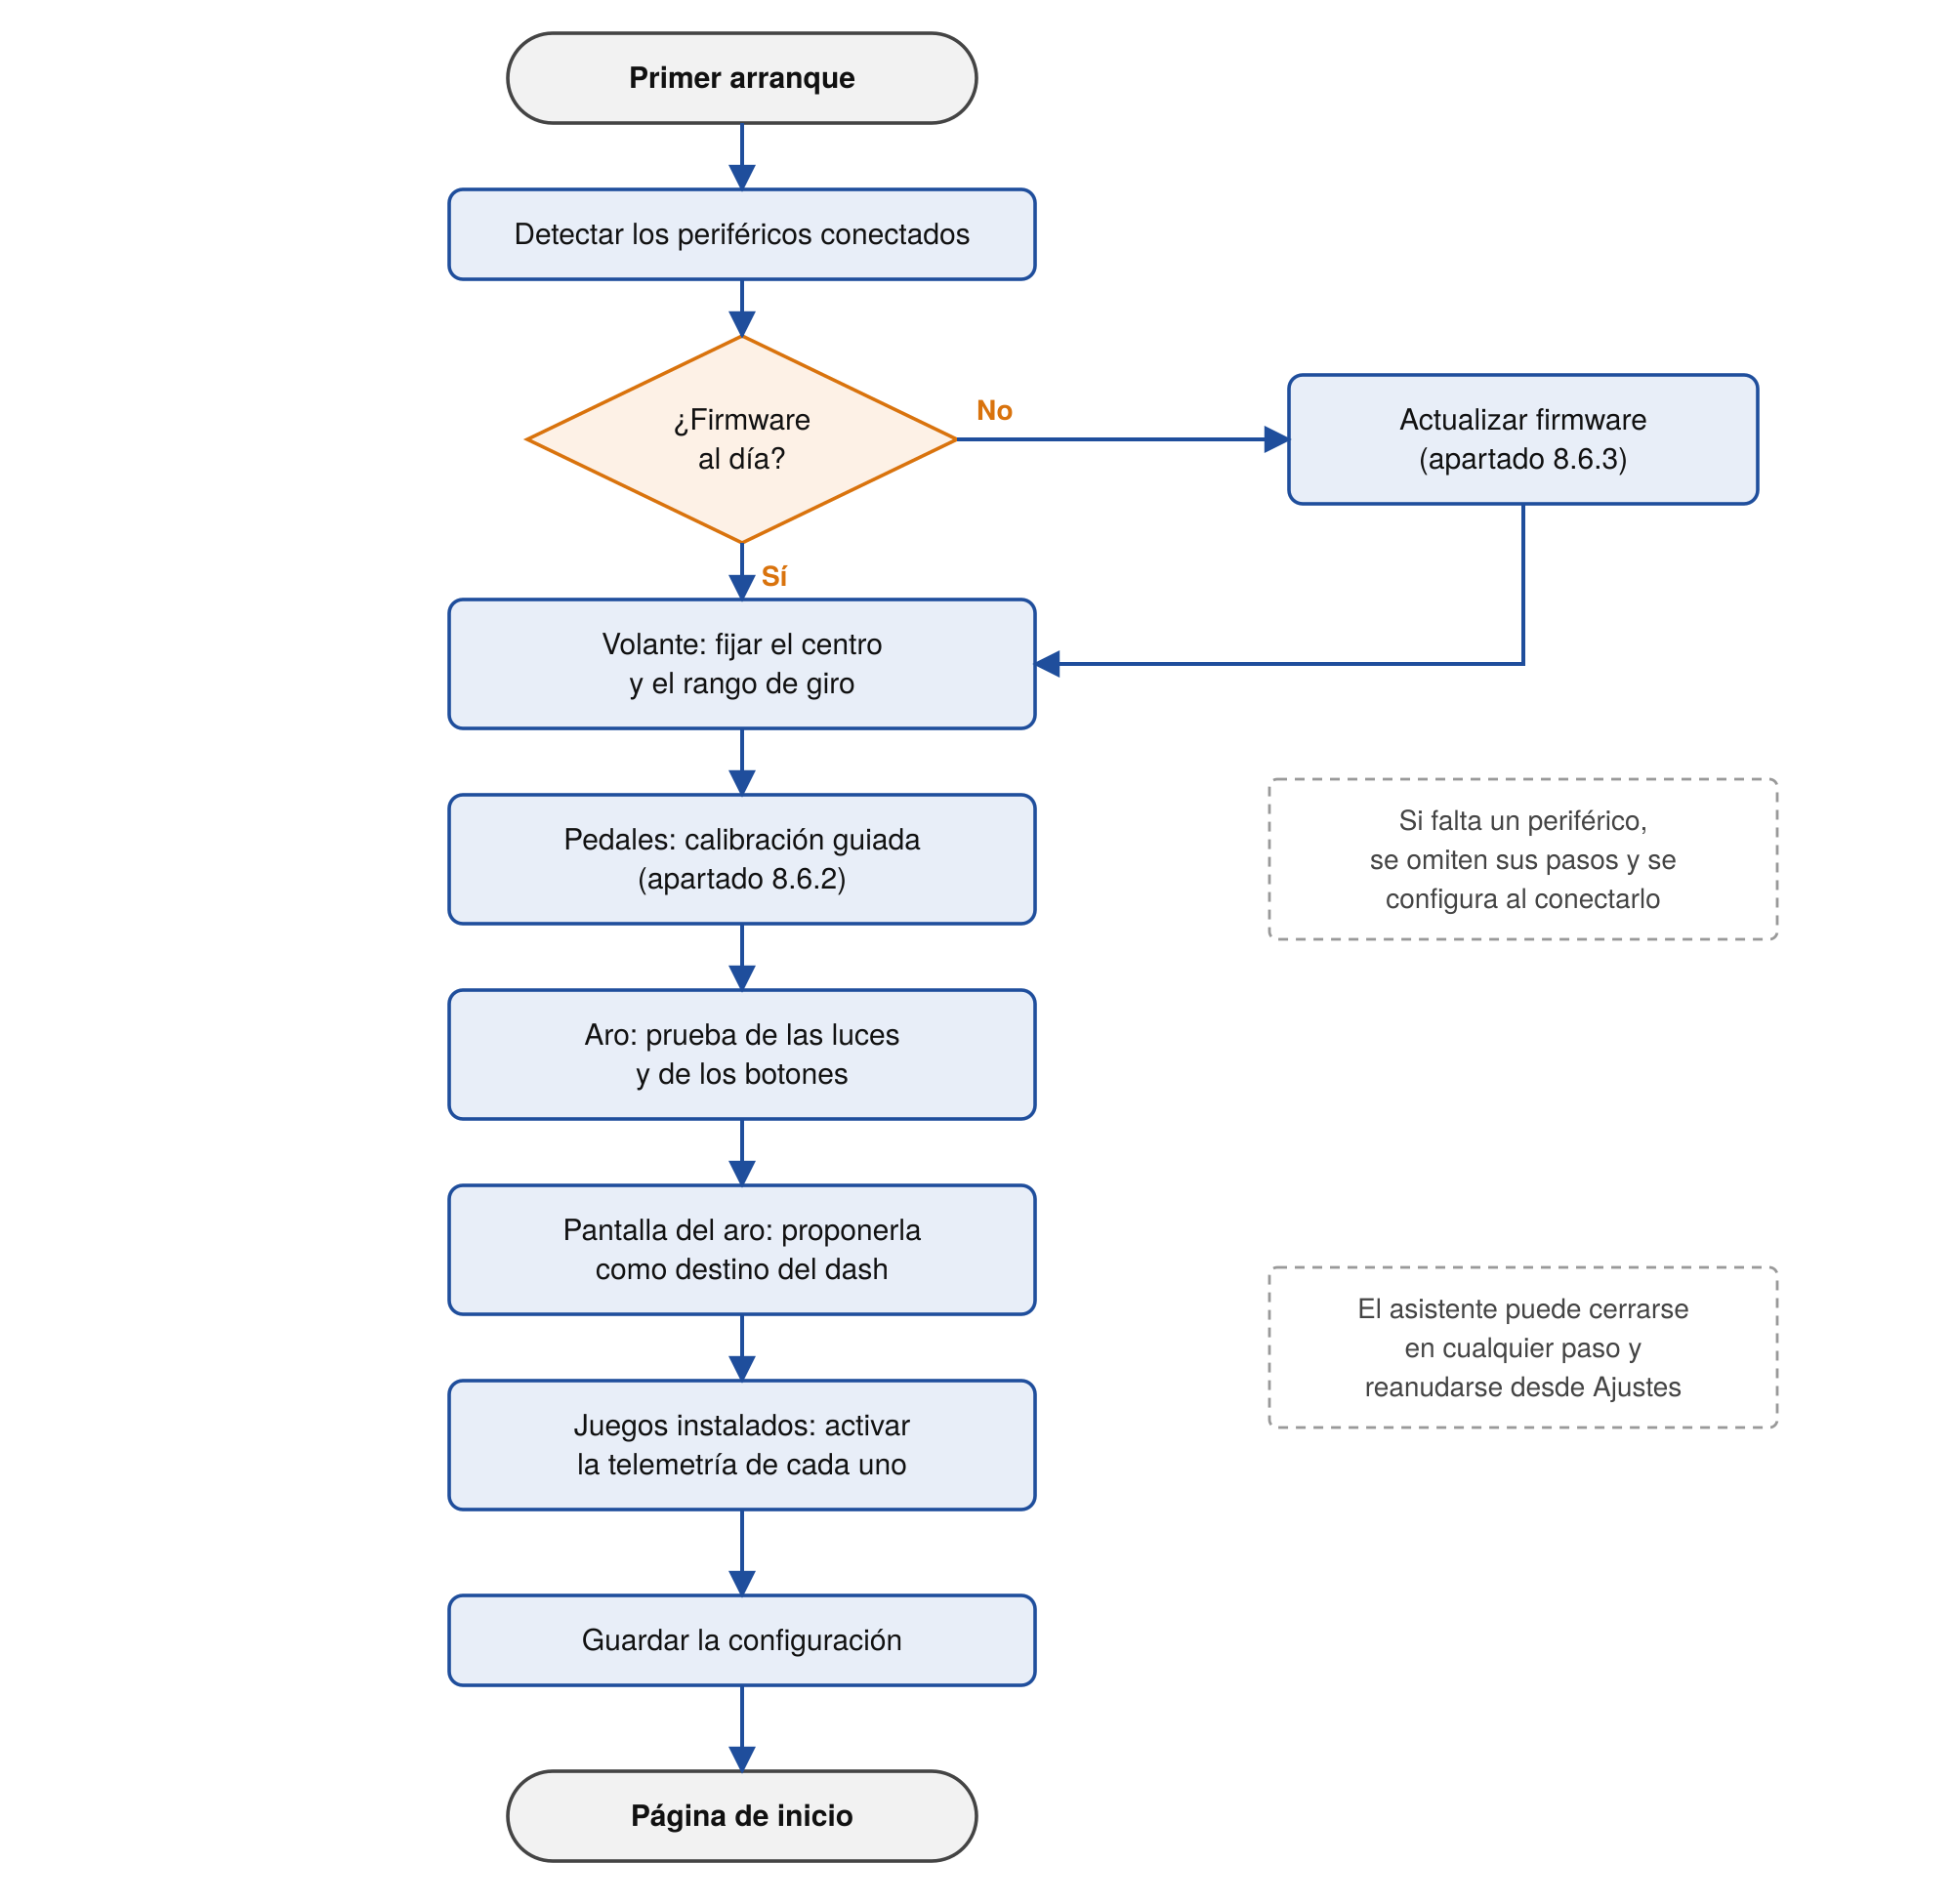
\includegraphics[width=0.8\textwidth]{img/ux-asistente.png}
	\caption{Flujo del asistente de primera configuración. (Fuente propia)}
	\label{fig:ux-asistente}
\end{figure}
El diseño del asistente responde a varias decisiones:

\begin{itemize}
	\item \textbf{Un paso por periférico, en orden de importancia.} El asistente empieza por el volante, sigue con los pedales y el aro, y termina con la pantalla del aro y los juegos. Cada paso pide una sola acción y muestra el resultado antes de pasar al siguiente, de modo que el piloto nunca tiene que recordar qué hizo antes.
	\item \textbf{El firmware primero.} Antes de configurar nada, el asistente comprueba que cada periférico tiene la última versión de firmware y, si no la tiene, ofrece actualizarlo. Así se evita calibrar un periférico con un firmware que va a cambiar justo después.
	\item \textbf{Adaptado a lo que hay conectado.} Si falta un periférico, el asistente omite sus pasos en lugar de detenerse, y lo configura cuando se conecte. Quien solo tiene la pedalera puede completar el asistente igual que quien tiene el equipo completo.
	\item \textbf{Las tareas fuera de la aplicación, explicadas.} Activar la telemetría depende de cada juego y no puede hacerlo la aplicación. Para ese paso, el asistente detecta los juegos instalados y explica, para cada uno, qué opción hay que activar.
	\item \textbf{Siempre se puede salir.} El asistente puede cerrarse en cualquier paso y reanudarse más tarde desde los ajustes de la aplicación.
\end{itemize}

\subsection{Calibración de los pedales}
\label{subsec:ux-calibracion}
La calibración indica a la pedalera dónde empieza y dónde acaba el recorrido de cada pedal y qué fuerza máxima se quiere aplicar en el freno (RF12). Sigue el caso de uso CU3 y su flujo se representa en la figura~\ref{fig:ux-calibracion}.

\begin{figure}[H]
	\centering
	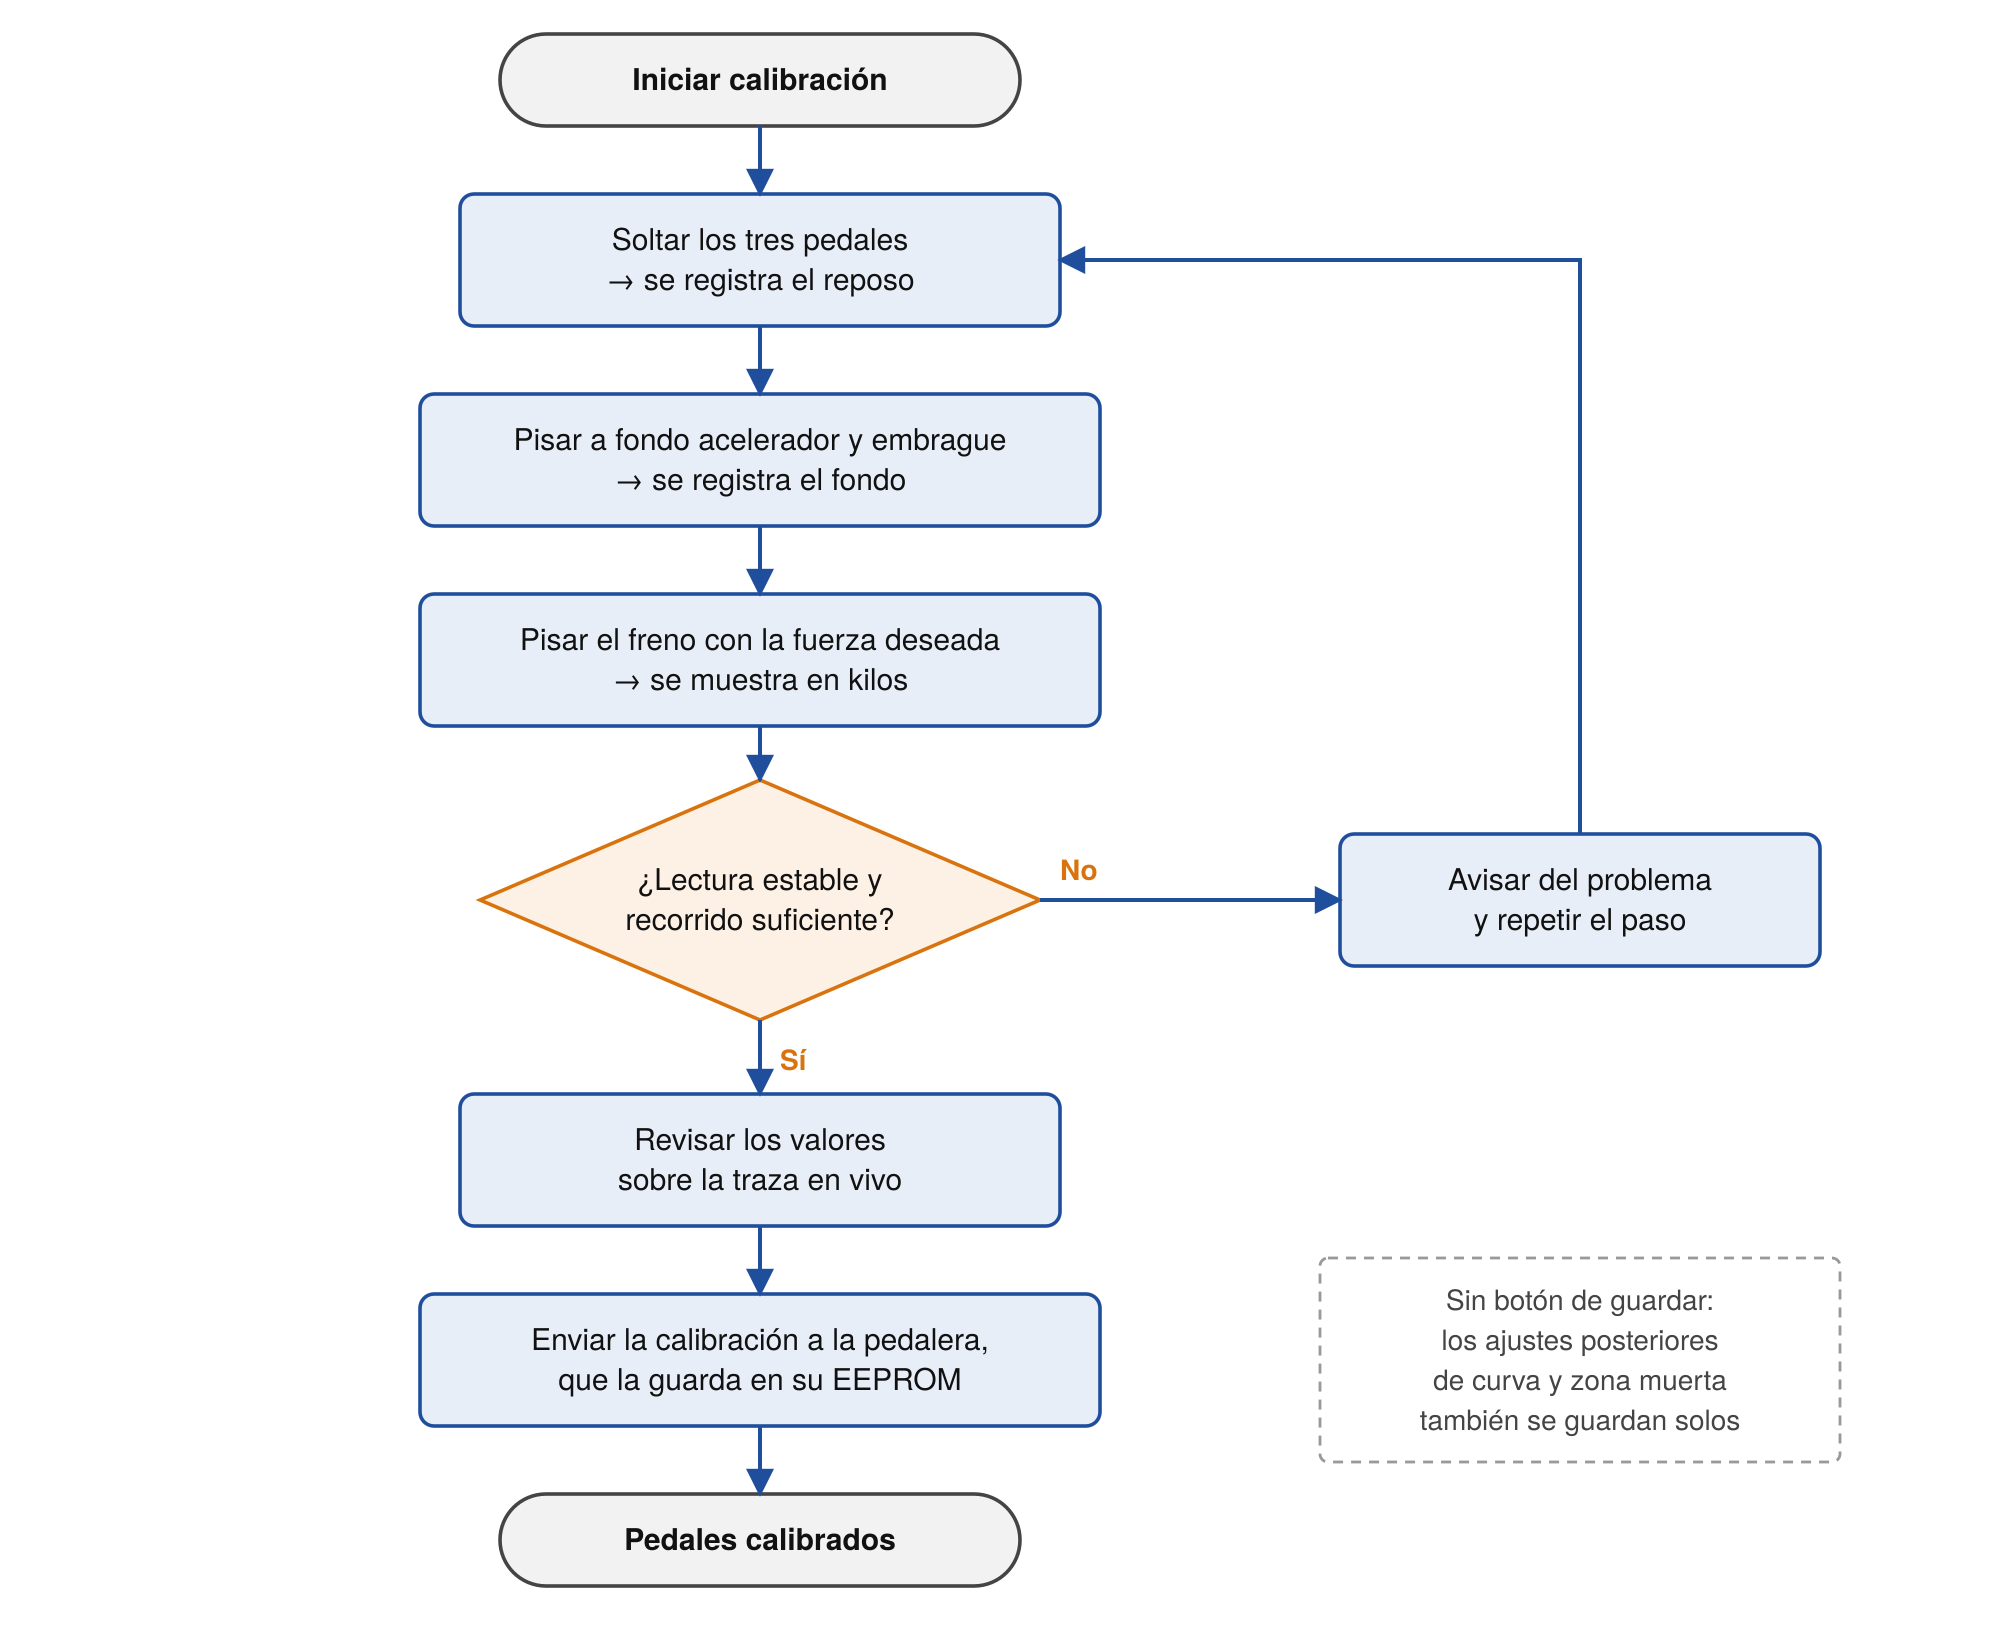
\includegraphics[width=0.8\textwidth]{img/ux-calibracion.png}
	\caption{Flujo de la calibración guiada de los pedales. (Fuente propia)}
	\label{fig:ux-calibracion}
\end{figure}

En una calibración tradicional, el usuario introduce a mano los valores mínimo y máximo de cada eje, unos números que no significan nada para un piloto. La calibración de VH SimGrid sustituye esos números por acciones físicas: soltar los pedales, pisarlos a fondo y frenar con la fuerza deseada. La aplicación toma cada lectura de la traza en vivo, de modo que el piloto ve en todo momento cómo responde el pedal mientras lo pisa, y después envía los valores a la pedalera con el mensaje de calibración (apartado~\ref{subsec:protocolo-pedalera-aro}).

El freno merece un tratamiento propio. Como mide la fuerza y no el recorrido, su fondo no es una posición física, sino la fuerza máxima con la que el piloto quiere frenar, que la aplicación muestra en kilos. Así el piloto decide la dureza del freno en una unidad que entiende, y puede reconocer de un vistazo si ha calibrado un freno blando o uno firme.

La aplicación comprueba además cada lectura antes de aceptarla. Si la señal es inestable, porque el pie aún se mueve, o el recorrido es demasiado corto para ser un pedal pisado a fondo, avisa del problema y repite el paso, en lugar de guardar una calibración que haría que el pedal no llegara nunca al 100~\%. Por último, la calibración y los ajustes que se hagan después, como la curva o la zona muerta, se guardan solos en la pedalera, sin un botón de guardar que el piloto pueda olvidar pulsar (RF14).

\subsection{Actualización de firmware}
\label{subsec:ux-firmware}
Actualizar el firmware de un microcontrolador suele exigir herramientas específicas, poner la placa en modo de grabación a mano y saber qué fichero corresponde a cada dispositivo. VH SimGrid reduce todo eso a una sola decisión del piloto: aceptar o no la actualización (RF32). El flujo, que sigue el caso de uso CU5, se muestra en la figura~\ref{fig:ux-firmware}.

\begin{figure}[H]
	\centering
	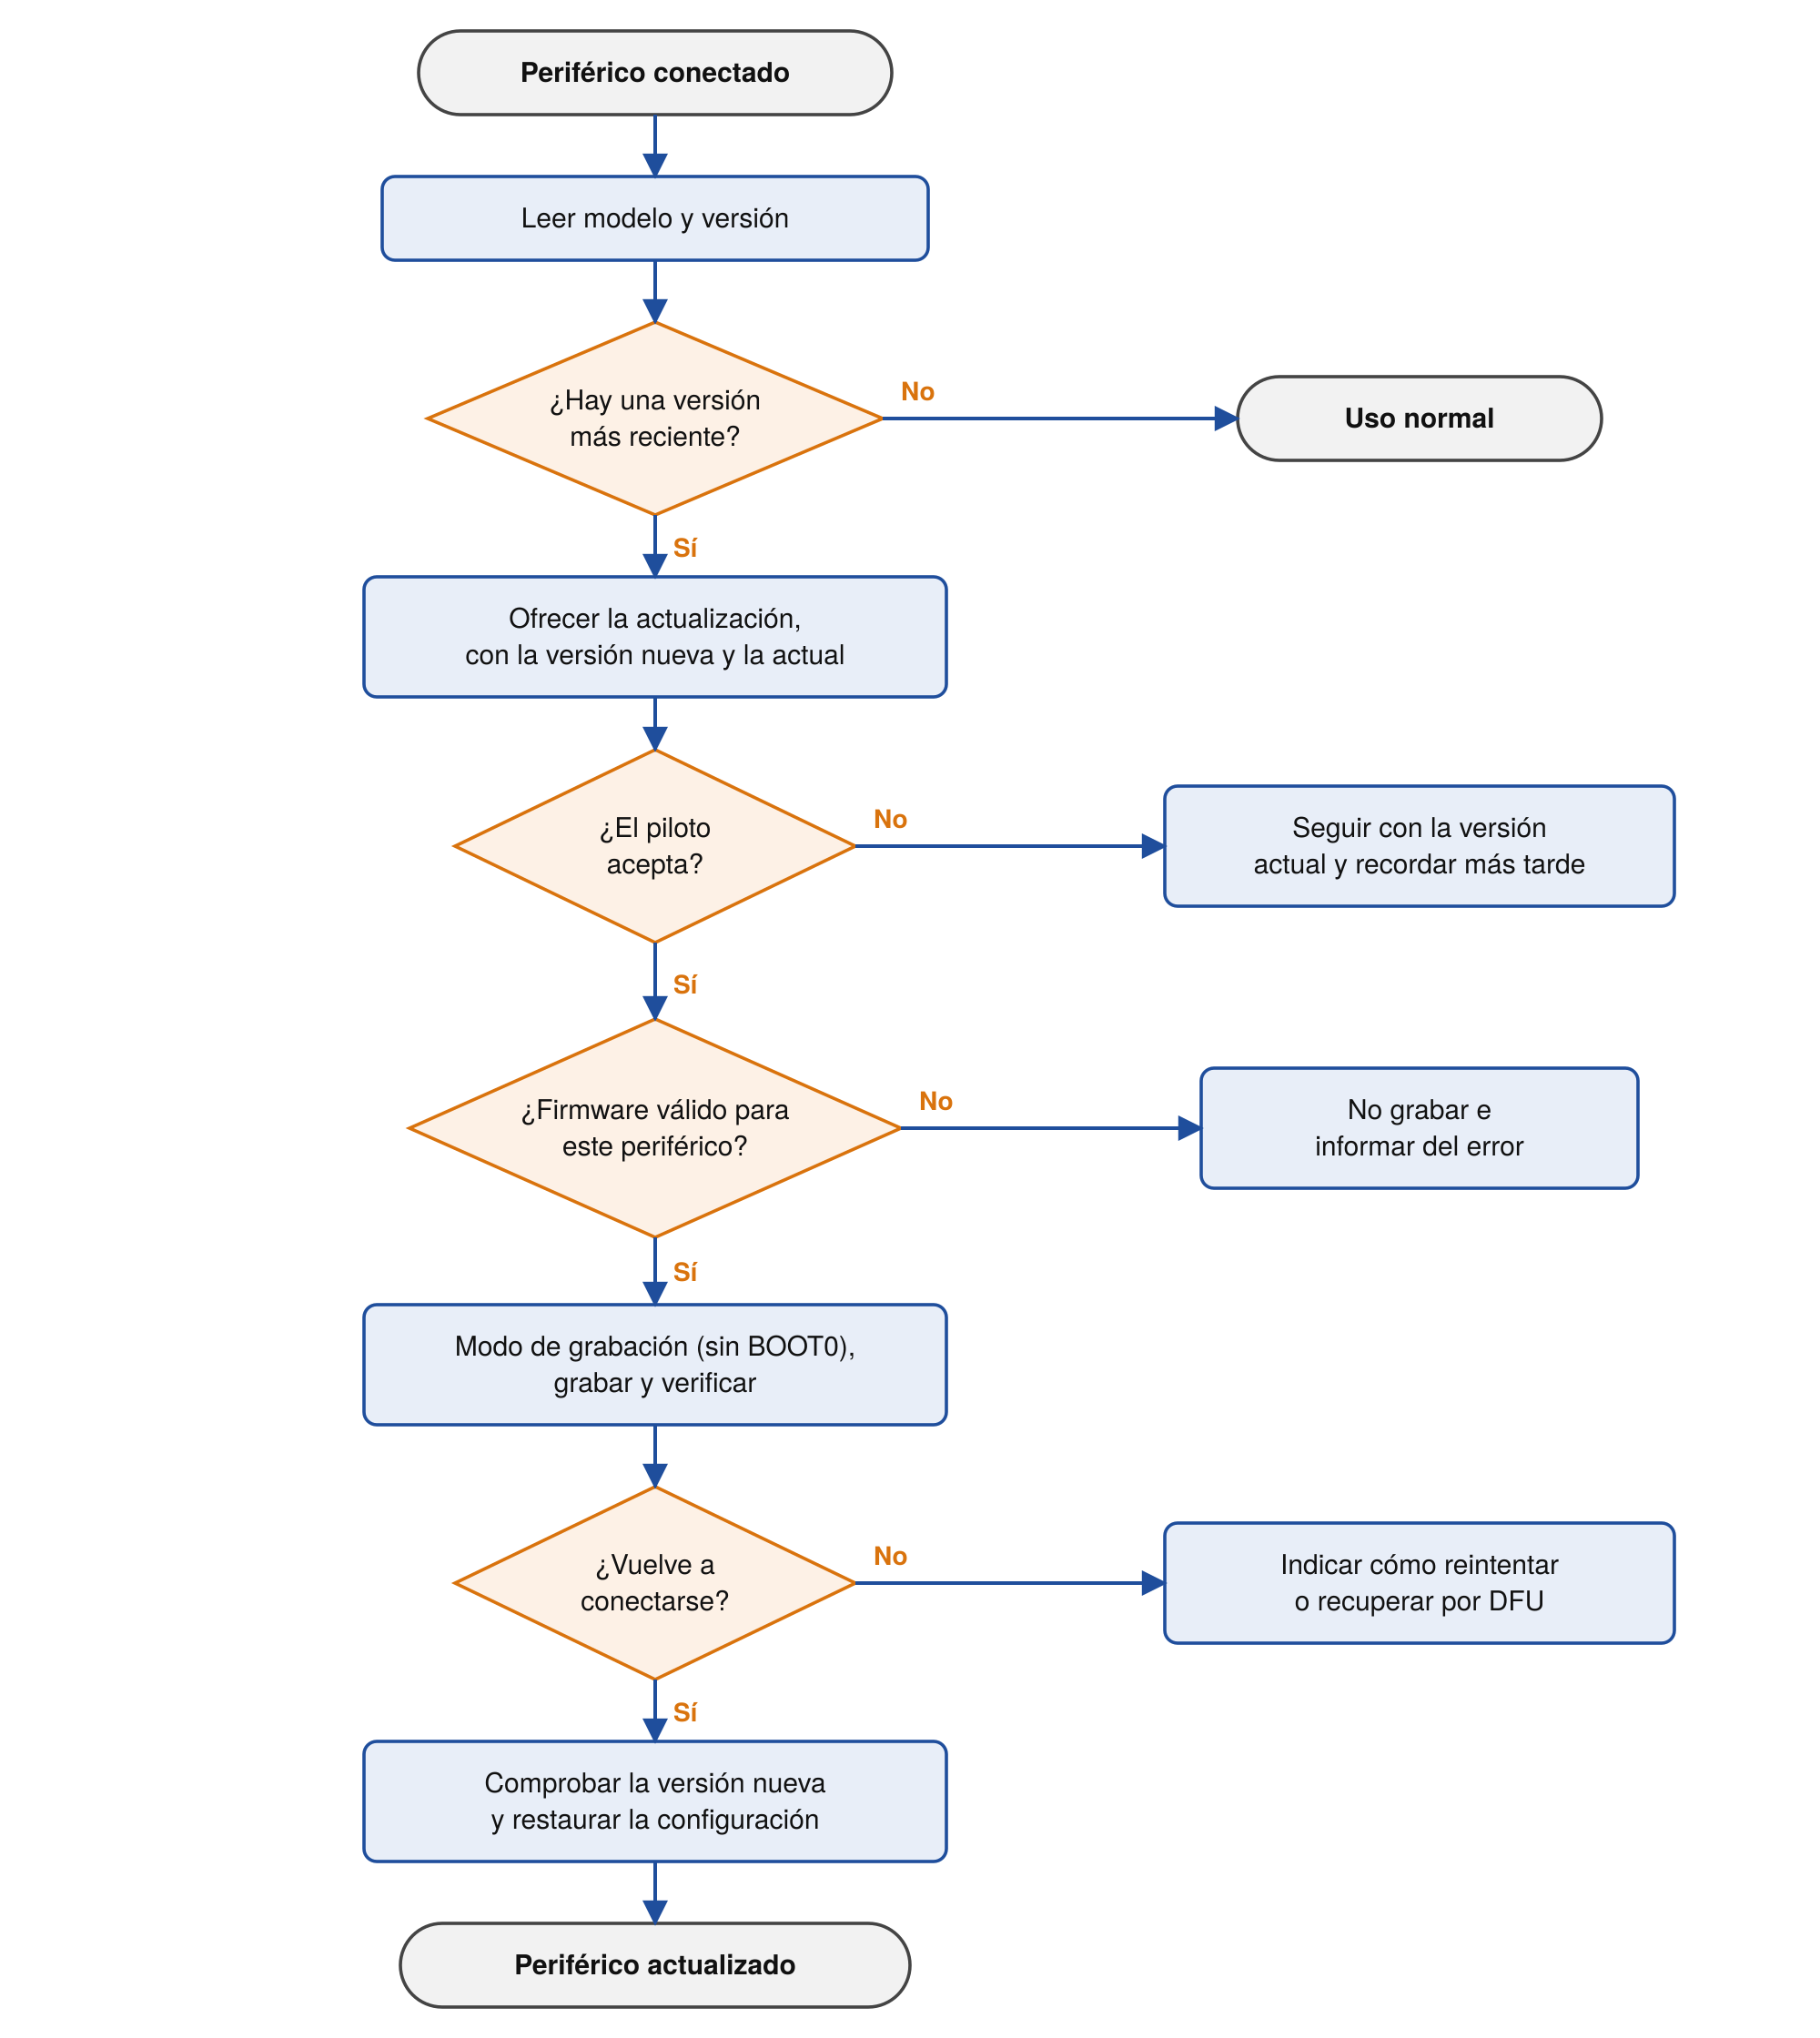
\includegraphics[width=0.75\textwidth]{img/ux-firmware.png}
	\caption{Flujo de la actualización de firmware de un periférico. (Fuente propia)}
	\label{fig:ux-firmware}
\end{figure}

Las decisiones de diseño más relevantes son las siguientes:

\begin{itemize}
	\item \textbf{Ofrecer, no imponer.} La aplicación compara la versión del periférico con la que incluye al conectarlo, y si hay una más reciente lo comunica y deja la decisión al piloto, mostrando ambas versiones. Si la pospone, el periférico sigue funcionando con su versión actual, y la aplicación lo recuerda más adelante. De este modo, una actualización nunca interrumpe una sesión.
	\item \textbf{Sin intervención física.} La aplicación pone ella misma el periférico en modo de grabación mediante una orden de su canal de configuración. En la base, esto evita abrir la carcasa para colocar el puente BOOT0, y en la pedalera y el aro, instalar herramientas externas.
	\item \textbf{Comprobar antes de grabar.} La aplicación elige el firmware según la identidad USB del periférico y comprueba que el fichero le corresponde y no está dañado. Si no supera la comprobación, no se graba, porque un firmware equivocado podría dejar el periférico inutilizable (RNF15).
	\item \textbf{Conservar la configuración.} Tras la grabación, la aplicación vuelve a conectar el periférico, comprueba la nueva versión y le restaura la configuración del usuario, de modo que el piloto no tiene que volver a calibrar nada (RNF24).
	\item \textbf{Un camino de recuperación.} Si el periférico no vuelve a conectarse, la aplicación indica cómo reintentar la grabación y, como último recurso, cómo recuperarlo por DFU, la única operación que requiere la intervención del constructor (CU6).
\end{itemize}

\subsection{Perfiles automáticos}
\label{subsec:ux-perfiles}
Cada juego, e incluso cada coche, se conduce mejor con unos ajustes distintos: un GT3 pide un \textit{force feedback} y un rango de giro diferentes a los de un monoplaza o un coche de rally. Los perfiles automáticos evitan que el piloto tenga que cambiar estos ajustes a mano cada vez que cambia de juego o de coche (RF31). Su funcionamiento se representa en la figura~\ref{fig:ux-perfiles}.

\begin{figure}[H]
	\centering
	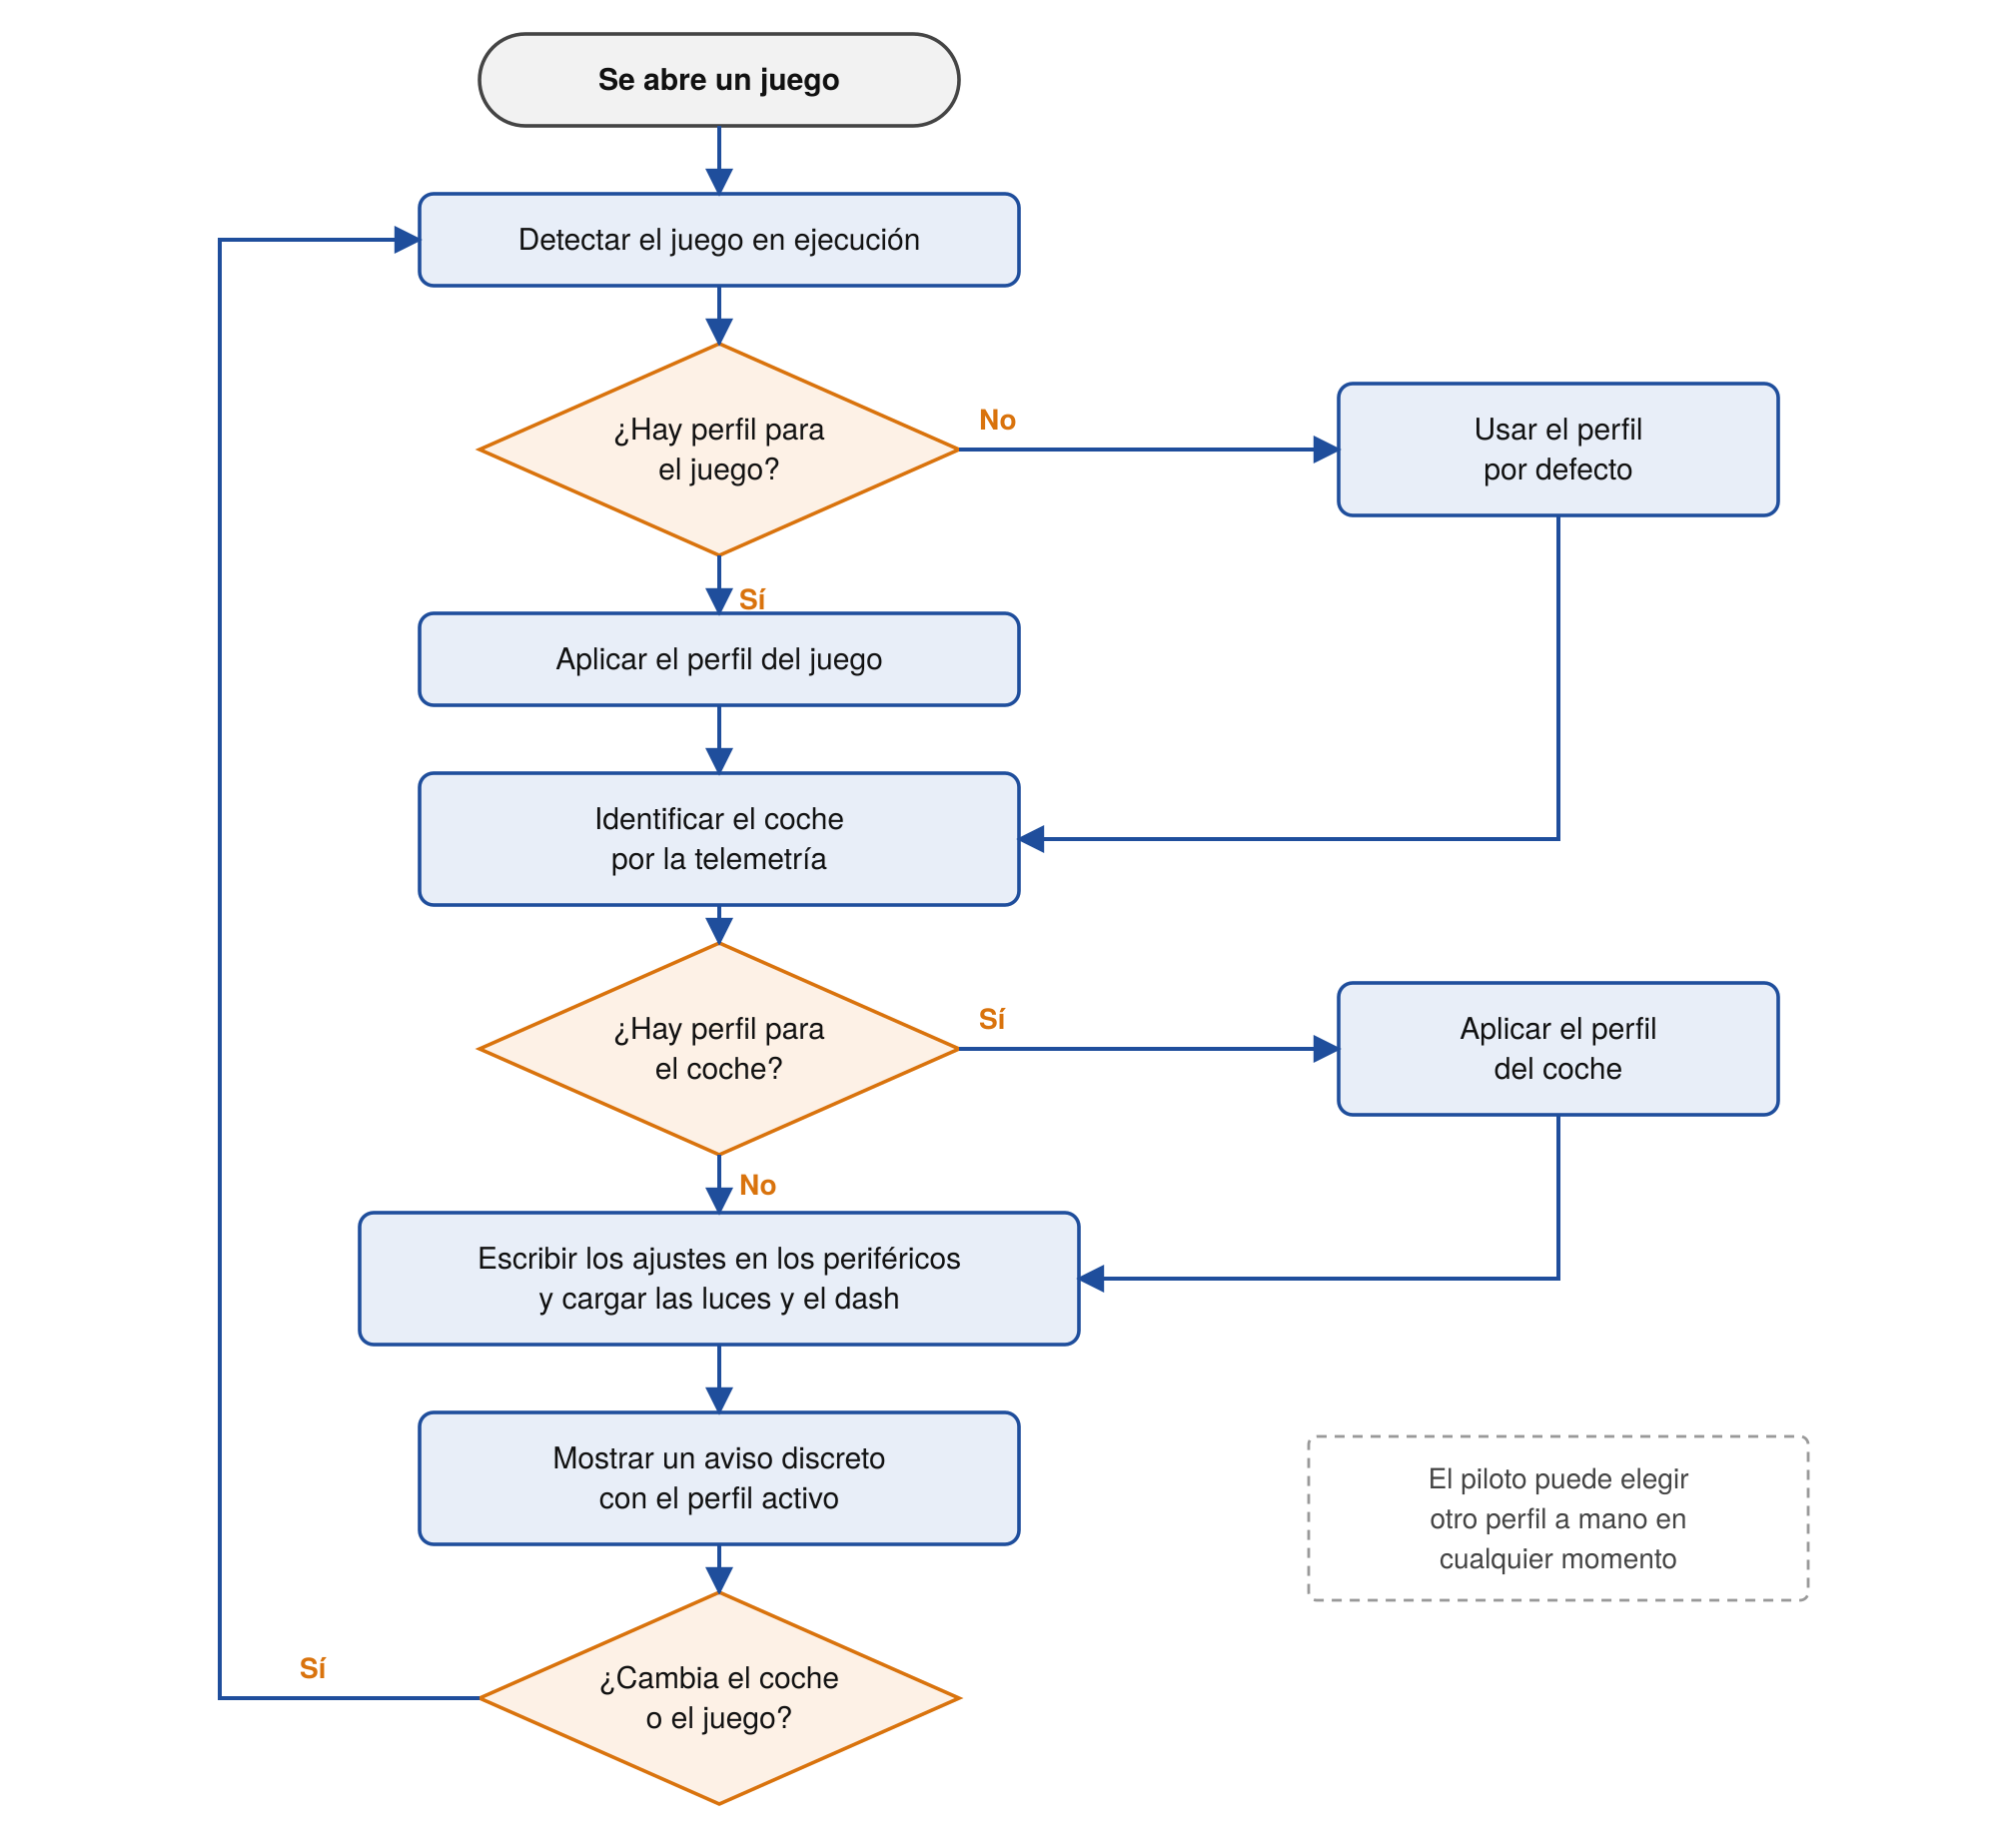
\includegraphics[width=0.8\textwidth]{img/ux-perfiles.png}
	\caption{Flujo de la aplicación automática de perfiles. (Fuente propia)}
	\label{fig:ux-perfiles}
\end{figure}

La selección del perfil se hace en dos niveles, del más general al más concreto. Cuando la aplicación detecta que se ha abierto un juego, aplica el perfil asociado a ese juego o, si no tiene ninguno, el perfil por defecto. Después, cuando la telemetría identifica el coche, comprueba si existe un perfil específico para él y, si existe, lo aplica en lugar del anterior. Este orden permite que el piloto configure solo lo que necesita: un perfil por juego cubre la mayoría de los casos, y los perfiles por coche quedan para las excepciones.

Aplicar un perfil no se limita a los ajustes de los periféricos. Con ellos se cargan también la asignación de luces del aro y el \textit{dash} asociado, que se abre en la pantalla del aro (RF20 y RF27), de modo que todo el equipo cambia a la vez. El proceso se repite cada vez que cambia el coche o el juego.

Como toda decisión automática, el cambio de perfil debe ser visible y reversible. La aplicación muestra un aviso discreto con el nombre del perfil aplicado, que informa al piloto sin interrumpirle, y el piloto puede elegir otro perfil a mano en cualquier momento, desde la aplicación o desde la pantalla del aro (RF25).


\section{Interfaces de usuario (UI)}
\subsection{Estructura general}
\subsection{Página de inicio}
\subsection{Página de configuración de la base}
\subsection{Página de configuración del aro}
\subsection{Página de configuración de la pedalera}
\subsection{Biblioteca de dash y editor}
\subsection{Ingeniero de pista}
\subsection{Análisis de la telemetría}
\subsection{Ajustes de la aplicación}

\section{Guía de estilos}
\subsection{Paleta de colores}
\subsection{Tipografía}
\subsection{Iconografía}
\subsection{Componentes reutilizables}

\section{Diseño de pruebas y validación}